%!TEX TS-program = xelatex
\documentclass[10pt,table,a4]{article}\usepackage[]{graphicx}\usepackage[]{color}

\usepackage{alltt}
\usepackage{graphicx}
\usepackage{gensymb}
\usepackage[top=1cm, bottom=1.5cm, left=1.2cm, right=1.2cm]{geometry}
\usepackage[font=small]{caption}
\usepackage{adjustbox}
\usepackage{fancyhdr}
\usepackage{layout}
%\usepackage{booktabs}
%\usepackage{kpfonts}
\usepackage[explicit]{titlesec}
\usepackage{wrapfig}
\usepackage{tcolorbox}
\usepackage{xcolor}
\usepackage{setspace}
\usepackage{parskip}
\usepackage{tikz}
\usepackage{fontspec}
\usepackage{anyfontsize}
\usepackage{hyperref}
\usepackage{multicol}
\usepackage{datetime}
\usepackage{fixltx2e}
\usepackage[sfdefault]{ClearSans}

% Colours
\definecolor{Yellow1}{RGB}{252, 190, 14}
\definecolor{Yellow2}{RGB}{252, 190, 54}
\definecolor{Yellow3}{RGB}{254, 238, 207}

\definecolor{OffBlack}{RGB}{61,61,60}
\definecolor{LightGray}{RGB}{208,208,208}

\definecolor{ColRed}{RGB}{244,123,115}
\definecolor{ColOrange}{RGB}{253,226,145}
\definecolor{ColYellow}{RGB}{255,255,204}
\definecolor{ColGreen}{RGB}{195,214,155}

\pagestyle{fancy}
\fancyhf{}
\fancyhead[R]{\thepage}
\renewcommand{\headrulewidth}{0pt}

\newcolumntype{P}[1]{>{\centering\arraybackslash}p{#1}}


\newcommand{\nearr}[1]{$\color{#1}\nearrow$}
\newcommand{\searr}[1]{$\color{#1}\searrow$}
\newcommand{\uparr}[1]{$\color{#1}\uparrow$}




\setlength{\parskip}{10pt}

%\pagenumbering{gobble}

\newcommand*{\PageHeadingSingleLine}{%
	\begin{tikzpicture}[remember picture,overlay]
	\node[anchor=north west,minimum width=.375cm,minimum height=1.2cm,fill=Yellow1] (RB) at (-1.2,1.2){\Large };
	\node[text=OffBlack, right of=RB, xshift = 18cm, yshift=0.75cm] at (0,0){\thepage};
	\end{tikzpicture}}
\newcommand*{\PageHeadingDoubleLine}{%
	\begin{tikzpicture}[remember picture, overlay]
	\node[anchor=north west,minimum width=.375cm,minimum height=1.9cm,fill=Yellow1] (RB) at (-1.2,1.2){\Large };
	\node[text=OffBlack, right of=RB, xshift = 18cm, yshift=0.6cm] at (0,0){\thepage};
	\end{tikzpicture}}
\newcommand{\HeaderSingle}[1]{
	\PageHeadingSingleLine 
	
	\vspace{-1.2cm}
	{\Large\textbf{#1}}
	\vspace{.2cm}}
\newcommand{\HeaderDouble}[2]{
	\PageHeadingDoubleLine
	
	\vspace{-1.2cm}
	{\Large\textbf{#1 \\[2pt] #2}}
	\vspace{.45cm}}
\newcommand*{\SectionHeadingBox}[1]{%
	\begin{tikzpicture}[remember picture, overlay]
	\node[anchor=north west,minimum width=.375cm,minimum height=#1,fill=Yellow1] (RB) at (-1.2,-16){\Large };
	\end{tikzpicture}
	\vspace{.8cm}}
\newcommand{\SectionHeading}[2]{
	\SectionHeadingBox{3cm}
	
	\vspace{15.7cm}
	\textbf{{\Huge #1 \\[6pt]\Huge #2}}}
\newcommand{\SectionHeadingDouble}[3]{
	\SectionHeadingBox{4cm}
	
	\vspace{15.7cm}
	\textbf{{\Huge #1 \\[6pt]\Huge #2\\[6pt]\Huge #3}}}
\newcommand{\PageFooterFirst}{% The number indicates the sector..... 
	\begin{tikzpicture}[remember picture, overlay]
	\node[text=OffBlack,above = .8cm, left = 6.4cm,font=\bf\small,align=center] at (current page.south){1-INTRODUCTION};
	\node[text=LightGray,above = .8cm, left = 2.73cm,font=\bf\small,align=center] at (current page.south){| 2-CURRENT EXPOSURE};
	\node[text=LightGray,above = .8cm, left = 0.495cm,font=\bf\small,align=center] at (current page.south){| 3-5YR TREND};
	\node[text=LightGray,above = .8cm, left = -2.94cm,font=\bf\small,align=center] at (current page.south){| 4-EXPOSURE IN 5YRS};
	\node[text=LightGray,above = .8cm, left = -6cm,font=\bf\small,align=center] at (current page.south){| 5-PHYSICAL RISKS};
	\node[text=LightGray,above = .8cm, left = -9.43cm,font=\bf\small,align=center] at (current page.south){| 6-COMPANY RESULTS};	
	\node[left=6.35cm,minimum width = 2.8cm, minimum height =0.01cm, fill = Yellow1] at (current page.south){};
	\end{tikzpicture}
}
\newcommand{\PageFooterSecond}{% The number indicates the sector..... 
	\begin{tikzpicture}[remember picture, overlay]
	\node[text=LightGray,above = .8cm, left = 6.4cm,font=\bf\small,align=center] at (current page.south){1-INTRODUCTION};
	\node[text=OffBlack,above = .8cm, left = 2.73cm,font=\bf\small,align=center] at (current page.south){| 2-CURRENT EXPOSURE};
	\node[text=LightGray,above = .8cm, left = 0.495cm,font=\bf\small,align=center] at (current page.south){| 3-5YR TREND};
	\node[text=LightGray,above = .8cm, left = -2.94cm,font=\bf\small,align=center] at (current page.south){| 4-EXPOSURE IN 5YRS};
	\node[text=LightGray,above = .8cm, left = -6cm,font=\bf\small,align=center] at (current page.south){| 5-PHYSICAL RISKS};
	\node[text=LightGray,above = .8cm, left = -9.43cm,font=\bf\small,align=center] at (current page.south){| 6-COMPANY RESULTS};	
	\node[left=2.73cm,minimum width = 3.65cm, minimum height =0.01cm, fill = Yellow1] at (current page.south){};
	\end{tikzpicture}
}
\newcommand{\PageFooterThird}{% The number indicates the sector..... 
	\begin{tikzpicture}[remember picture, overlay]
	\node[text=LightGray,above = .8cm, left = 6.4cm,font=\bf\small,align=center] at (current page.south){1-INTRODUCTION};
	\node[text=LightGray,above = .8cm, left = 2.73cm,font=\bf\small,align=center] at (current page.south){| 2-CURRENT EXPOSURE};
	\node[text=OffBlack,above = .8cm, left = 0.495cm,font=\bf\small,align=center] at (current page.south){| 3-5YR TREND};
	\node[text=LightGray,above = .8cm, left = -2.94cm,font=\bf\small,align=center] at (current page.south){| 4-EXPOSURE IN 5YRS};
	\node[text=LightGray,above = .8cm, left = -6cm,font=\bf\small,align=center] at (current page.south){| 5-PHYSICAL RISKS};
	\node[text=LightGray,above = .8cm, left = -9.43cm,font=\bf\small,align=center] at (current page.south){| 6-COMPANY RESULTS};	
	\node[left=0.468cm,minimum width = 2.35cm, minimum height =0.01cm, fill = Yellow1] at (current page.south){};
	\end{tikzpicture}
}
\newcommand{\PageFooterFourth}{% The number indicates the sector..... 
	\begin{tikzpicture}[remember picture, overlay]
	\node[text=LightGray,above = .8cm, left = 6.4cm,font=\bf\small,align=center] at (current page.south){1-INTRODUCTION};
	\node[text=LightGray,above = .8cm, left = 2.73cm,font=\bf\small,align=center] at (current page.south){| 2-CURRENT EXPOSURE};
	\node[text=LightGray,above = .8cm, left = 0.495cm,font=\bf\small,align=center] at (current page.south){| 3-5YR TREND};
	\node[text=OffBlack,above = .8cm, left = -2.94cm,font=\bf\small,align=center] at (current page.south){| 4-EXPOSURE IN 5YRS};
	\node[text=LightGray,above = .8cm, left = -6cm,font=\bf\small,align=center] at (current page.south){| 5-PHYSICAL RISKS};
	\node[text=LightGray,above = .8cm, left = -9.43cm,font=\bf\small,align=center] at (current page.south){| 6-COMPANY RESULTS};	
	\node[left=-2.97cm,minimum width = 3.45cm, minimum height =0.01cm, fill = Yellow1] at (current page.south){};
	\end{tikzpicture}
}
\newcommand{\PageFooterFifth}{% The number indicates the sector..... 
	\begin{tikzpicture}[remember picture, overlay]
	\node[text=LightGray,above = .8cm, left = 6.4cm,font=\bf\small,align=center] at (current page.south){1-INTRODUCTION};
	\node[text=LightGray,above = .8cm, left = 2.73cm,font=\bf\small,align=center] at (current page.south){| 2-CURRENT EXPOSURE};
	\node[text=LightGray,above = .8cm, left = 0.495cm,font=\bf\small,align=center] at (current page.south){| 3-5YR TREND};
	\node[text=LightGray,above = .8cm, left = -2.94cm,font=\bf\small,align=center] at (current page.south){| 4-EXPOSURE IN 5YRS};
	\node[text=OffBlack,above = .8cm, left = -6cm,font=\bf\small,align=center] at (current page.south){| 5-PHYSICAL RISKS};
	\node[text=LightGray,above = .8cm, left = -9.43cm,font=\bf\small,align=center] at (current page.south){| 6-COMPANY RESULTS};	
	\node[left=-6.05cm,minimum width = 3.05cm, minimum height =0.01cm, fill = Yellow1] at (current page.south){};
	\end{tikzpicture}
}
\newcommand{\PageFooterSixth}{% The number indicates the sector..... 
	\begin{tikzpicture}[remember picture, overlay]
	\node[text=LightGray,above = .8cm, left = 6.4cm,font=\bf\small,align=center] at (current page.south){1-INTRODUCTION};
	\node[text=LightGray,above = .8cm, left = 2.73cm,font=\bf\small,align=center] at (current page.south){| 2-CURRENT EXPOSURE};
	\node[text=LightGray,above = .8cm, left = 0.495cm,font=\bf\small,align=center] at (current page.south){| 3-5YR TREND};
	\node[text=LightGray,above = .8cm, left = -2.94cm,font=\bf\small,align=center] at (current page.south){| 4-EXPOSURE IN 5YRS};
	\node[text=LightGray,above = .8cm, left = -6cm,font=\bf\small,align=center] at (current page.south){| 5-PHYSICAL RISKS};
	\node[text=OffBlack,above = .8cm, left = -9.43cm,font=\bf\small,align=center] at (current page.south){| 6-COMPANY RESULTS};	
	\node[left=-9.4cm,minimum width = 3.4cm, minimum height =0.01cm, fill = Yellow1] at (current page.south){};
	\end{tikzpicture}
}

\setmainfont{ClearSans}
\color{OffBlack}


% Box with a shaded border
\newtcolorbox{shadedbox}{colback=Yellow3}

\begin{document}
	\section*{} % Front Page
	
	
	\thispagestyle{empty}
	\pagecolor{Yellow1}
	
	\vspace{-2.6cm}
	
	\begin{tikzpicture}[remember picture, overlay]
	\vspace{7cm}
	\node[below=-.6cm] (CN) at (current page.north){\adjincludegraphics[height=15cm,trim={0cm 0cm 0cm 2cm},clip]{ReportGraphics/FrontPageCA.jpeg}
	};
	
	\node[below = 4.5cm, right,align = left, white, text width=10cm](TN) at (current page.center){
		\Huge{\textbf{2° SCENARIO ANALYSIS}}\\[10pt]
		
		\vspace{2cm}
		{\baselineskip=20pt\Huge\raggedright{\textbf{InsuranceCompanyName}\par}}};
	
	\node[below = 3.8cm,right= .12cm, minimum width = .8cm, minimum height =0.3cm,fill= OffBlack] at (current page.center){};
	
	\end{tikzpicture}
	
	
	\begin{tikzpicture}[remember picture,overlay]
	\node[anchor=south west, yshift = 0cm ,minimum width=21.6cm,minimum height=4cm,fill=white] (RB) at (current page.south west){};
	\node[left= 7cm, above=1.cm] (WS) at (current page.south){\adjincludegraphics[height=1.8cm,trim={0cm 0cm 0cm 0cm},clip]{ReportGraphics/Logo_front}};
	\node[ below = 1.8cm, minimum width = 3.5cm, minimum height =0.05cm, fill = Yellow1] at (WS){};
	\end{tikzpicture}
	
	
	
	
	
	\newpage
	\pagecolor{white}
	\section*{} % Disclaimer p2
	
	\begin{center}
		\textbf{2Dii PACTA MODEL}
		
		\textbf{Important Information \& Legal Disclaimer: MODEL OUTPUT REPORTS}
		
		\textbf{IMPORTANT INFORMATION}
		
	\end{center}
	
	
	The 2Dii PACTA Model generates a limited `point in time' estimate of the relative alignment of the Revealed Plans of Securities in the Scope versus the economic trends embodied in the 2C Scenario(s), as identified by external data and scenario providers. 
	
	\textbf{EXCLUSION OF LIABILITY: }TO THE EXTENT PERMITTED BY LAW WE WILL NOT BE LIABLE TO ANY USER FOR ANY LOSS OR DAMAGE, WHETHER IN CONTRACT, TORT (INCLUDING NEGLIGENCE), BREACH OF STATUTORY DUTY OR OTHERWISE, EVEN IF FORESEEABLE, ARISING UNDER OR IN CONNECTION WITH USE OF OR RELIANCE ON ANY INFORMATION, DATA OR CONTENT OBTAINED VIA OUR SERVICES, INCLUDING (WITHOUT LIMITATION) THE MODELLING OUTPUTS STATED IN THIS REPORT.
	
	\textbf{No forecast or prediction: }The PACTA Model does not purport to generate, nor does this Report contain or comprise, statements of fact, forecasts or predictions. The PACTA Model provides a `point in time' analysis of economic and commercial variables that are inherently dynamic and variable over time. 2Dii neither makes nor implies any representation regarding the likelihood, risk or expectation of any future matter. To the extent that any statements made or information contained in this Report might be considered forward-looking in nature, they are subject to risks, variables and uncertainties that could cause actual results to differ materially. You are cautioned not to place undue reliance on any such forward-looking statements, which reflect our assumptions only and those of our data and scenario providers as of the date of modelling.
	
	\textbf{No financial advice: }The information contained in this Report does not comprise, constitute or provide, nor should it be relied upon as, investment or financial advice, credit ratings, an advertisement, an invitation, a confirmation, an offer or a solicitation, or recommendation, to buy or sell any security or other financial, credit or lending product or to engage in any investment activity, or an offer of any financial service. This Report does not purport to quantify risk to the portfolio (or any part thereof), nor make any representation in regards to the performance, strategy, prospects, creditworthiness or risk associated with any investment, nor their suitability for purchase, holding or sale in the context of any particular portfolio. The Modelling Outputs reflected in this Report are provided with the understanding and expectation that each investor will, with due care, conduct its own investigation and evaluation of each security or other instrument that is under consideration for purchase, holding or sale. 
	
	\textbf{Scope Securities: }The PACTA Model is limited in its scope and application. It does not consider all securities across all sectors, nor all securities within those sectors. The PACTA Model applies only to the Scope Securities set out in the Methodology Statement, as updated from time to time. 
	
	\textbf{2C Scenario(s): }The PACTA Model will apply one or more 2C Scenarios, as set out in the Methodology Statement. The choice of any 2C Scenarios should not be taken as any endorsement of those scenarios, nor any statement as to the accuracy or completeness of those scenarios' methodologies or assumptions, nor as a general preference of those scenarios over any other economic scenarios. The analysis provided by the PACTA Model may be carried out using other economic scenarios, and users must form their own view as to the decarbonisation scenarios, trajectories and models that are most appropriate to their portfolio. No explicit or implicit assumption is made in relation to the current or future alignment of the 2C Scenarios with climate-related policies of any government at international, national or sub-national level.
	
	\textbf{TCFD: }Use of the PACTA Modelling Tool may support you in initiatives undertaken with regard to the Recommendations of G20 Financial Stability Board's Taskforce on Climate-related Financial Disclosures (TCFD). However, its use in isolation does not purport to provide TCFD compliance. 
	
	
	\newpage
	\section*{} % Exec Summary p3
	\HeaderSingle{EXECUTIVE SUMMARY}
	
	\begin{multicols}{2}
		\textbf{This report provides a 2°C scenario analysis of the investment portfolio.} 
		
		It responds to the recommendations of the G20 Financial Stability Board Task Force on Climate-related Financial Disclosures (TCFD). The California Department of Insurance engaged the 2° Investing Initiative to undertake a scenario analysis of the investment portfolios of insurers operating in California with over \$100 million in premiums.
		
		The outputs provided in this report - based on the scope summarized in the table on the right - provide an analysis of the portfolio relative to an economic transition consistent with limiting global warming to 	2°C above pre-industrial levels. The analysis answers three questions: 
		
		\begin{enumerate}
			\item{What is the current exposure of the portfolio to economic activities affected by the transition to a low-carbon economy? (Section 2)}
			\item{Does the portfolio increase or decrease its alignment with a 2°C transition over the next 5 years? (Section 3)}
			\item{What is the expected future exposure to high- and low-carbon economic activities? (Section 4)}
		\end{enumerate}
		
		The analysis covers two asset classes: listed equity and `fixed income', which includes corporate bonds as well as bonds of the largest government and municipal power producers. Notably excluded from this analysis (shown in grey below) are insurance subsidiaries of insurance companies in the equity portfolios, sovereign bonds, and alternative investments. 

		
		\begin{center}
			{\rowcolors{2}{white}{Yellow3}
				\setlength{\tabcolsep}{10pt} % Default value: 6pt
				\renewcommand{\arraystretch}{1.5} % Default value: 1
				\begin{tabular}{ p{.35\linewidth} p{.49\linewidth} }
					\hline
					\multicolumn{2}{c}{\textbf{Scope of Analysis}} \\
					\hline
					Insurer Name & InsuranceCompanyName \\ 
					Size of Portfolio & SizeofPortfolio \\ 
					Scenario & IEA 2° Scenario \\ 
					Geography - \newline Financial Assets & Global \\ 
					Geography - \newline Economic Assets & Global \\ 
					Asset Class & AssetClass \\ 
					Peers & 672 Insurers operating in CA with premiums over \$100 million \\
					Portfolio Timestamp & 12.31.2016 \\ 
					Date of Analysis & TodaysDate \\ 
					\hline
				\end{tabular}
			}
			
		\end{center}
		
		
		
		The graph on the bottom left shows the share of the total fixed income and equity investments included in the analysis, referred to as ``the portfolio" (light blue plus dark blue sections). Within this portfolio, the 2°C scenario analysis focuses on the fossil fuel, power, and automotive sectors (dark blue), which 	account for roughly 90\% of energy-related CO\textsubscript{2}-emissions in a typical portfolio. The chart on the bottom right shows the share of companies active in each of these sectors in the analyzed portfolio.
		
		
		
		
		
		
		\vspace{1.2cm}
		
		
	\end{multicols}	
	
	
	
	\begin{multicols}{2}
		
		\textbf{The figure below shows the share of the total fixed income and equity investments included in the analysis.} AnalysisCoverage\% of investments are included in the analysis (``the portfolio"). %ClimateRelevant\% are in the fossil fuels, power, and automotive sectors.
		
		\textbf{The figure below shows the share of the fossil fuels, power, and automotive sectors in the portfolio.}
		
	\end{multicols}	
	
	\begin{multicols}{2}
		\centering{\adjincludegraphics[width = .9\linewidth,trim={0cm 0.2cm 0cm .2cm},clip]{CAFigures/Fig01}	}
		
		\centering{\adjincludegraphics[width = .9\linewidth,trim={0cm 0.2cm 0cm .2cm},clip]{CAFigures/Fig02}	}
		
	\end{multicols}	
	
	\newpage
	\section*{} % Exec Summary p4
	\HeaderSingle{EXECUTIVE SUMMARY}
	
	\begin{multicols}{2}
		
		\textbf{The figure below shows the estimated percent of the portfolio currently exposed to activities across the fossil fuel, power, and automotive sectors.}
		
		The results show the share of the portfolio potentially exposed to transition risks in the fossil fuel, power, and automotive sectors. The results are calculated by first calculating the exposure of the portfolio to companies active in each of these sectors, and then calculating the specific technology exposure on the basis of the breakdown of those companies' asset base.      
		
		The percentages are compared to the market portfolio. The market portfolio results are calculated based on the exposure of the global universe of assets in both the listed equity and fixed income markets to the fossil fuel, power, and automotive sectors.
		
		A value higher than the market portfolio suggests the portfolio is currently more exposed to transition risk than the market, on average. A value lower than the market portfolio suggests the portfolio is less exposed, all other things being equal. As will be outlined in the following sections, the extent to which these risks will materialize is likely to be at least in part a function of the evolution of the companies' activities over time. 
		
		\textit{Note: In the graphs below, coal is shown separately to highlight those results. In the graphs below and throughout this report, ``ICE" refers to Internal Combustion Engine (gasoline and diesel) vehicles.}
		
	\end{multicols}
	
	\textbf{Current exposure of the fixed income portfolio to high-carbon and low-carbon activities, as a \% of the portfolio, compared to the fixed income market}	
	
	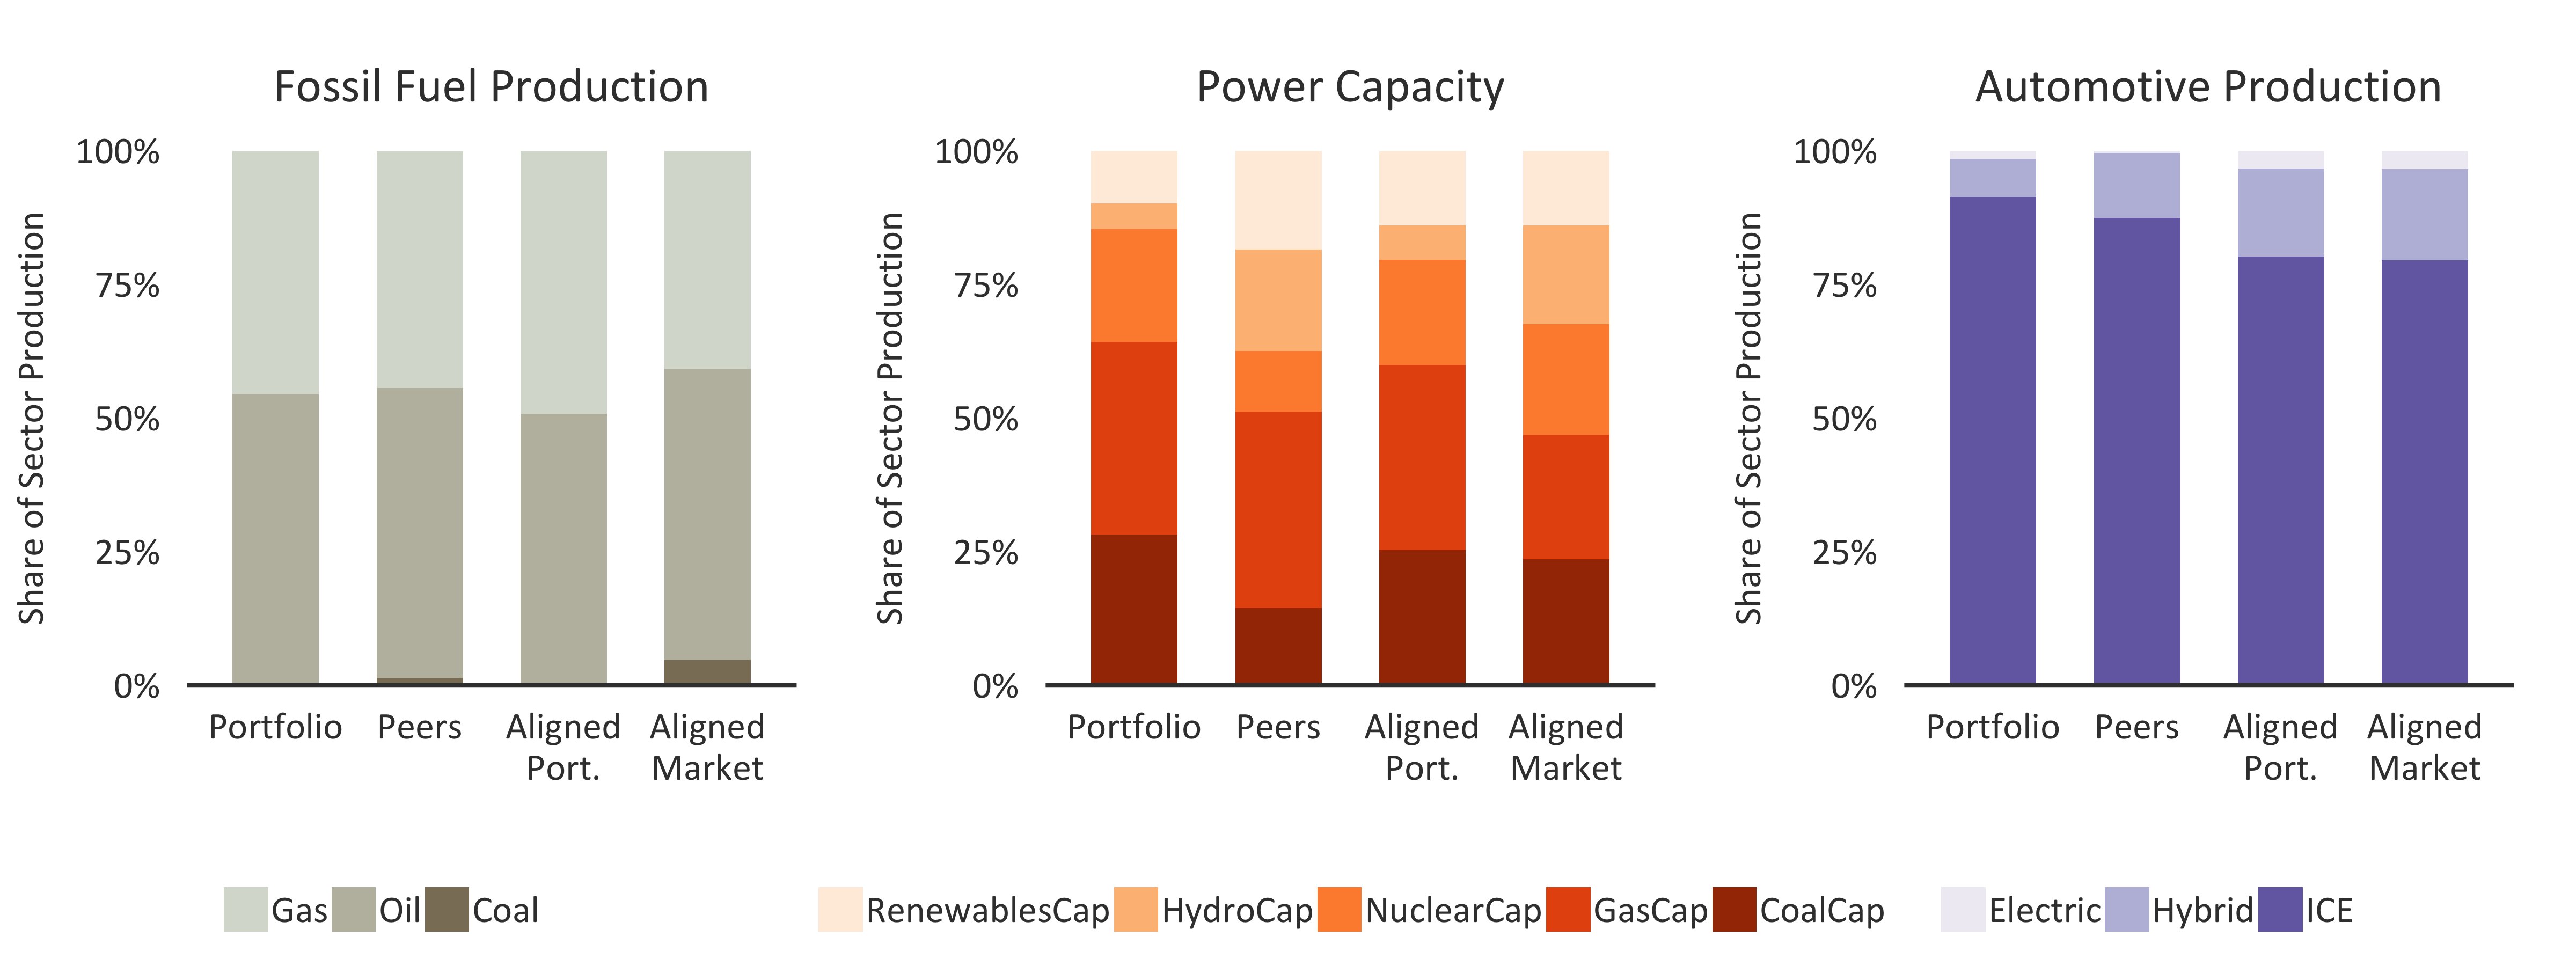
\includegraphics[trim = {0 0cm 0 0cm},width=1\linewidth]{CAFigures/Fig05} 
	
	
	\textbf{Current exposure of the equity portfolio to high-carbon and low-carbon activities, as a \% of the portfolio, compared to the equity market} 
	
	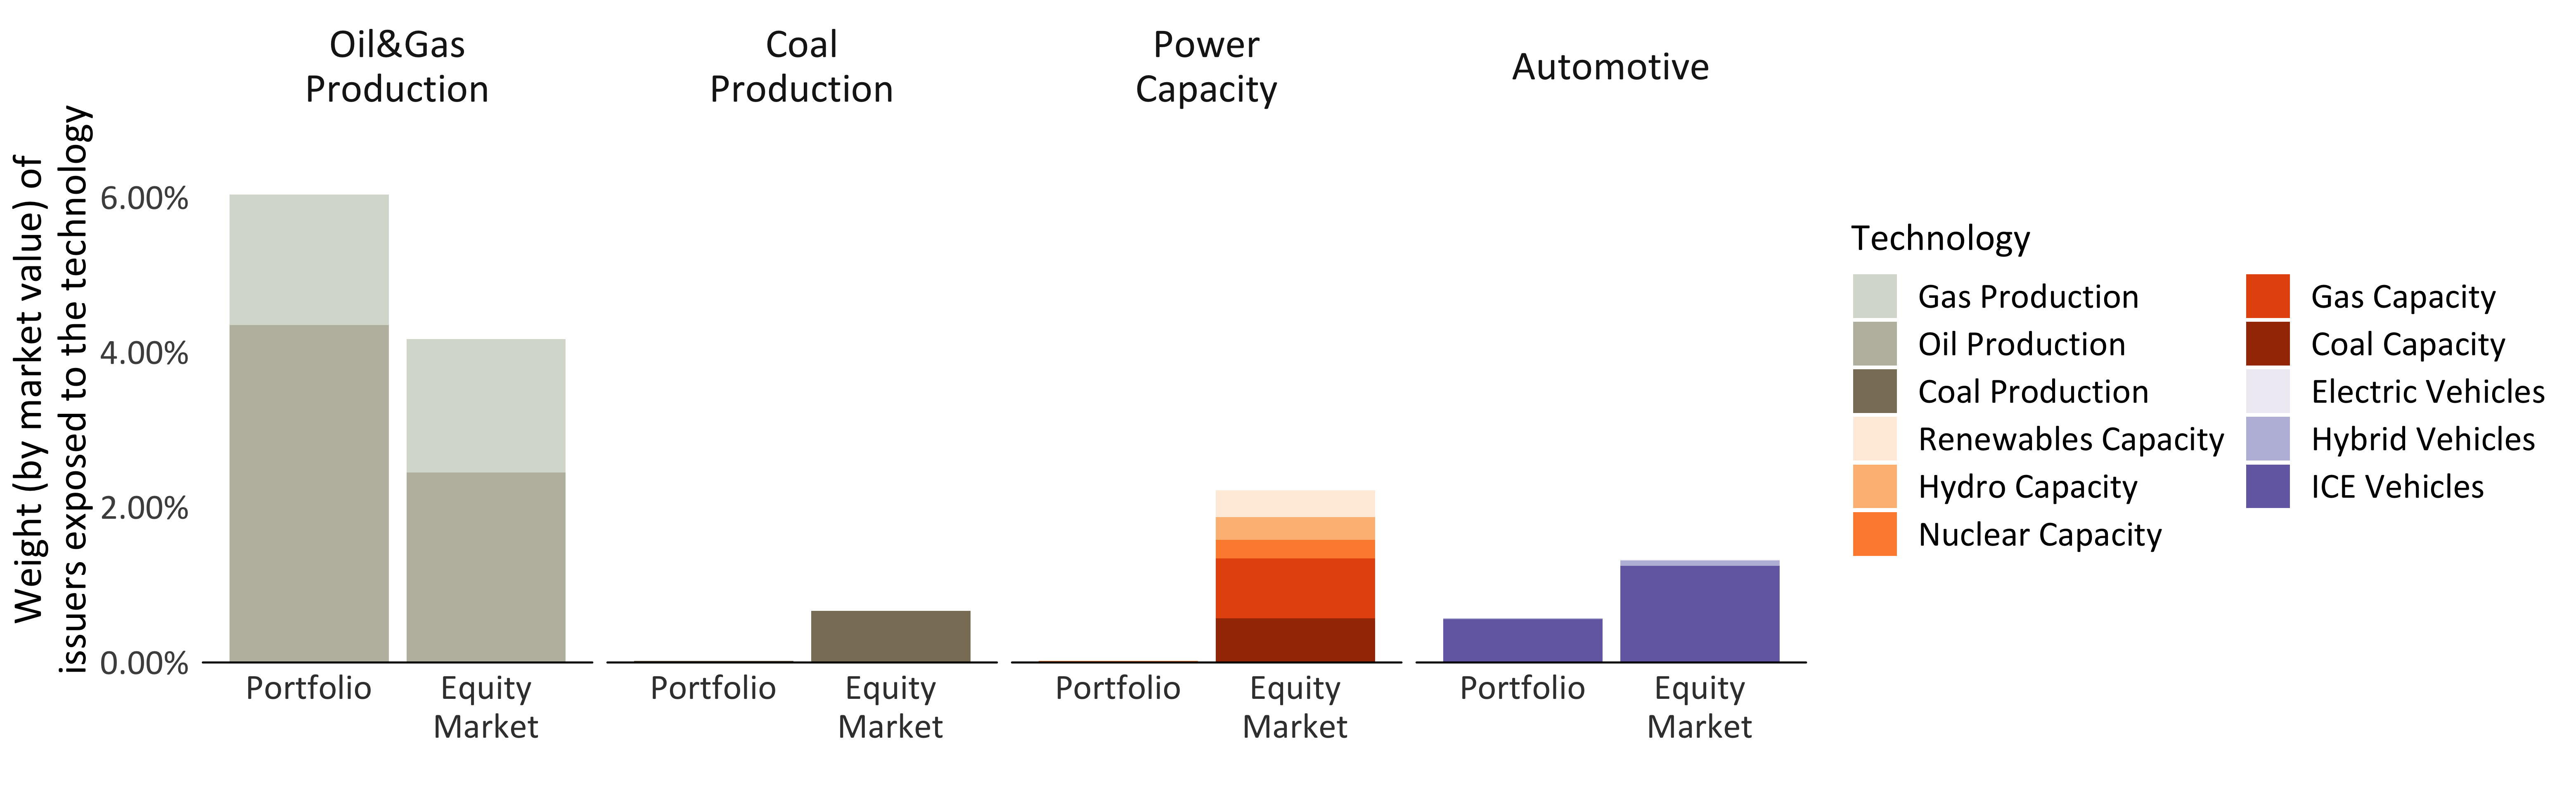
\includegraphics[trim = {0 0cm 0 0cm},width=1\linewidth]{CAFigures/Fig04}		
	
	
	
	\newpage
	\section*{} % 1st Section
	\SectionHeading{SECTION 1:}{INTRODUCTION}
	
	
	\newpage
	\section*{} % Report Contents p6
	\HeaderSingle{REPORT CONTENTS}
	
	\begin{multicols}{2}
		
		\textbf{This report provides a 2°C scenario analysis, following the recommendations of the G20's Financial Stability Board Task Force on Climate-related Financial Disclosures (TCFD). Specifically, it seeks to inform the reader about four issues.}
		
		\begin{enumerate}
			\item{\textbf{What is the current exposure of the portfolio to economic activities affected by the transition to a low-carbon economy? (Section 2) }
			}
			
			The first part of the report summarizes the exposures of the portfolio (in terms of \% of the portfolio) to business activities potentially affected by the transition to a low-carbon economy and by extension to transition risk. Specifically, it will quantify the percent of the portfolio exposed to low-carbon and high-carbon activities across the fossil fuel, power, and automotive sectors. The results will be presented relative to the market portfolio. For fossil fuels, the analysis will also show this portfolio's exposure relative to the distribution of fossil fuel exposures of all insurance companies included in this analysis.  
			
			\item{\textbf{Does the portfolio increase or decrease its alignment with a 2°C transition over the next 5 years? (Section 3)}
			}
			
			The second part of the report will quantify the extent to which the portfolio is building or reducing risk in terms of being aligned / misaligned with the 2°C scenario pathway over the next 5 years. The analysis will focus on technologies in the fossil fuel sector (oil production, gas production), electric power sector (coal power, gas power, nuclear power, renewables power), and automotive sector (internal combustion engine vehicles and electric vehicles). The analysis will compare the currently planned production or investment trend in the portfolio with the production or investment trend that would be required under the 2°C scenario. 
			
			\item{\textbf{What is the expected future exposure to high- and low-carbon economic activities based on the current revealed production and investment plans of the companies in the portfolio? (Section 4)}
			}
			
			Section 4 of this report will quantify the expected evolution of the portfolio’s exposure to high-carbon and low-carbon activities in 5 years (2023) based on the current revealed production and investment plans of companies in portfolio with business activities in the fossil fuel, power, and automotive sectors. The section will show the portfolio's expected future technology mix in each sector compared to the expected future technology mix of both the aggregated investment portfolio of all insurance companies included in this analysis and the 2° market benchmark.  
			
			\item{\textbf{What is driving the results? (Section 5)}}
			
			Section 5 will provide background on the securities and companies driving the results presented in the previous sections, including additional analysis on individual companies' profiles. 
			
			You will also be able to find further background information on the scenarios and modelling at the end of the report (Section 6).
			
			
		\end{enumerate}
		
		
	\end{multicols}
	
	%	\vspace{1cm}
	\begin{tikzpicture}[remember picture, overlay]
	\node[anchor=north west,minimum width=.375cm,minimum height=5.cm,fill=Yellow1] (ToC) at (-1.2,-.4){};
	\end{tikzpicture}	
	
	\begin{minipage}[t]{.5\linewidth}
		\textbf{Section 1: }Introduction\\
		
		\textbf{Section 2: }The current exposure\\
		
		\textbf{Section 3: }Trajectory of the portfolio relative to a 2°C scenario\\
		
		\textbf{Section 4: }The expected future exposure in 2023\\
		
		\textbf{Section 5: }Company exposure\\
		
		\textbf{Section 6: }Background to the model\\
	\end{minipage}
	
	\PageFooterFirst
	
	\newpage
	\section*{} %CONTEXT p7
	\HeaderSingle{CONTEXT}
	
	\begin{multicols}{2}
		\textbf{Background.} In June 2017, the G20 Financial Stability Board Task Force on Climate-related Financial Disclosures (TCFD) recommended that financial institutions perform scenario analysis on their portfolios to assess financial risks related to climate change. The TCFD grouped climate-related risks into two categories: physical and transition risks. Transition risks are risks generated by the policy, technology, market, and regulatory changes likely to accompany the transition to a low carbon economy. As part of its supervisory role, the California Department of Insurance engaged the 2° Investing Initiative (2Dii) to undertake a scenario analysis of the investment portfolios of insurance companies operating in California with more than \$100 million in premiums.  As part of this assessment, individual scenario analysis reports will be sent to insurers with the 100 largest investment portfolios, and any insurer operating in California can request their own report.
		
		\textbf{Goal.} The goal of the scenario analysis was to assess insurers' exposure to transition risk, individually and as a whole, based on their estimated current and future exposure to high-carbon and low-carbon activities. This report provides the results of the analysis for a single insurer portfolio.
		
		\textbf{Approach.} The key elements of the analysis are:
		
		\begin{itemize}
			\item{\textit{Current and planned production and investment trends.} Current and planned production (for the fossil fuel and automotive sector) and current installed capacity as well as new capacity additions (for the power sector) for the next 5 years were sourced from commercial business intelligence databases. These data providers collect forward-looking production and capacity data at the physical asset level, including gigajoules of oil by field, cars by model and factory, and new capacity by power plant. 2Dii maps this data to their immediate owners and parent company to generate a company's aggregate `current production profile' for each technology. These production plans are linked to the financial securities (equity and fixed income) issued by the company. The asset-level data used for this analysis was retrieved from data providers during the first half of 2017. See the `Important Considerations and Limitations' section at the end of the report for notes on interpreting power sector capacity data.}
			
			\item{\textit{Allocating the production of physical assets to financial assets.} Based on the share of total equity or debt held in a portfolio, the model allocates a portion of each corporate issuer's current production plans for each technology to the portfolio. Aggregated over all companies to the portfolio level, this is the portfolio's `current production profile' for a technology. This also defines the insurer's current `exposure' to each technology.}
			
			\item{\textit{From macro-level scenarios to micro-level targets. }To calculate production levels consistent with a climate scenario such as the IEA 2°C scenario, the model uses a `fair share' principle that applies the changes specified by the scenario for a given technology and region equally across all owners of physical assets in that technology's sector in the given region. This creates a set of alternative, forward-looking production and capacity profiles consistent with the scenario for each company and technology. These alternative profiles are then aggregated to the portfolio level to create the portfolio's `target production profile' under the scenario. This profile is used to determine the insurer's `target exposure' to a technology under the scenario. The `target exposure' does not assume any change in the composition of the portfolio: it models the changes in production and investment plans that are required across the different companies held in the portfolio in order to match the technology deployment described in the scenario. This report uses the scenarios of the International Energy Agency, specifically the 450S and the 2D scenario.} 
			
		\end{itemize}
		
		\textbf{Results of the scenario analysis.} The portfolio's `target profile' under the scenario can be compared to the portfolio's currently revealed production and investment plans for each technology to derive the exposure to transition risk as well as the extent to which the portfolio is projected to increase or decrease alignment with the 2°C scenario over the next 5 years. It is this analysis that forms the basis of the subsequent sections, with Section 6 providing further detail on the methodology.	
		\newline
		
	\end{multicols}
	
	\PageFooterFirst	
	\newpage
	\section*{} %CONTEXT p8
	\HeaderSingle{TRANSITION RISK FOR INVESTORS}
	\begin{multicols}{2}
		\textbf{What are transition risks?} Transition risks can be broadly defined as economic and financial risks associated with the transition to a low-carbon economy. The international community has defined a mandate to limit the man-made contribution to global warming to well below 2°C above pre-industrial levels. According to best available science, achieving this objective requires decarbonizing the economy in the course of this century. This decarbonization is set to have significant implications for high-carbon sectors, most prominent among which are the fossil fuel, power, and transport sectors, contributing the majority of global anthropogenic GHG emissions. 
		
		As the economy decarbonizes, companies that fail to properly anticipate this transition are set to be exposed to economic risks. Companies well-prepared for this transition in turn are set to capitalize from this economic opportunity. Similarly, economic risks may translate into financial risks in financial markets if these risks are not properly anticipated by financial market actors. 
		
		Crucially, the transition to a low-carbon economy is set to already have dramatic impacts in the short- and medium-term. By 2040, in only 22 years, global coal production is set to decline by 46\%, with a more accelerated decline expected in developed markets. Global coal power capacity in turn is similarly set to decline by 41\%. The production of gasoline and diesel vehicles (internal combustion engine or ICE vehicles) is set to decline by 21\%. This decline in high-carbon activity in turn will be accompanied by the commensurate deployment and growth of new technologies. Renewable power capacity and electric vehicle production in turn is set to nearly quadruple in volume by 2040. 
		
		Scenario analysis can help financial institutions assess and ultimately manage the risks and opportunities associated with the transition. In recognition of these risks, scenario analysis has been applied to date by hundreds of financial institutions as well as financial supervisors. It forms the basis of the recommendations of the FSB TCFD. The TCFD notes that ``forward-looking assessments of climate-related issues is important for investors and other stakeholders in understanding how vulnerable individual organizations are to transition and physical risks and how such vulnerabilities are or would be addressed. As a result, the Task Force believes that organizations should use scenario analysis to assess potential business, strategic, and financial implications of climate-related risks and opportunities and disclose those, as appropriate, in their annual financial filings" (TCFD Final Report, p. 33). 
		
		To clarify its scenario analysis recommendation, the Task Force explains, ``A key type of transition risk scenario is a so-called 2°C scenario, which lays out a pathway and an emissions trajectory consistent with holding the increase in the global average temperature to 2°C above pre-industrial levels" (TCFD Final Report, p. 35).
		
		It is this premise that forms the basis of this report, highlighting for the portfolio the current exposure to transition risks in the fossil fuel, power, and automotive sectors, the trends in the portfolio over time in these sectors relative to the 2°C scenario, and the expected future exposure on the basis of these trends. While these sectors do not represent all high-carbon activities and sectors, they account for both the largest share in a typical portfolio and the most significant contribution to climate change currently, as well as benefiting from well-developed scenario pathways.
		
		The report does not provide specific estimates as to the potential loss in value that may be realised in the portfolio should these risks materialize, which is obviously associated with significant uncertainty and myriad modelling assumptions. For any individual security, the potential loss may range from 0 to 100\% and may even be associated with positive returns, depending on the adaptive capacity of the company, the anticipation of the trend by financial markets, and the nature of a potential repricing. It is the proper anticipation of these risks that minimizes the loss that this report seeks to contribute to. 
		
		
		
	\end{multicols}
	
	
	\begin{center}
		{\setlength{\tabcolsep}{10pt} % Default value: 6pt
			\renewcommand{\arraystretch}{1} % Default value: 1
			\begin{tabular}{ p{.24\linewidth}| P{.24\linewidth}| P{.24\linewidth}}
				\hline
				\textbf{Technology} & \textbf{Total Volume Change by 2023} & \textbf{Total Volume Change by 2040} \\ 
				\hline
				Renewable Power & 69\% \nearr{ColGreen} & 354\% \uparr{ColGreen}\\
				Hydro Power & 13\% \nearr{ColGreen} & 59\% \nearr{ColGreen}\\
				Nuclear Power & 17\% \nearr{ColGreen} & 89\% \nearr{ColGreen}\\
				Gas Power & 8\% \nearr{ColGreen} & 31\% \nearr{ColGreen}\\
				Coal Power & -3\% \searr{ColRed} & -41\% \searr{ColRed}\\				
				\hline
				Oil Production & -2\% \searr{ColRed} & -23\% \searr{ColRed}\\
				Gas Production & 5\% \nearr{ColGreen} & 8\% \nearr{ColGreen}\\
				Coal Production & -11\% \searr{ColRed}& -46\% \searr{ColRed}\\ 
				\hline
				ICE Production & -9\% \searr{ColRed} & -21\% \searr{ColRed}\\
				Hybrid Production & 97\% \uparr{ColGreen} & 440\% \uparr{ColGreen}\\
				Electric Production & 105\% \uparr{ColGreen} & 352\% \uparr{ColGreen}\\
				\hline
			\end{tabular}
		}
	\end{center}
	
	\PageFooterFirst
	\newpage
	\section*{} % 2nd Section
	\SectionHeading{SECTION 2:}{THE CURRENT EXPOSURE}
	
	\newpage
	\section*{} % 2° SCENARIO - CURRENT EXPOSURE 2018 p10
	\HeaderDouble{CURRENT EXPOSURE}{COMPARISION TO MARKET}
	
	\begin{multicols}{2}

		\textbf{This page provides information on the estimated percent of the portfolio currently exposed to activities across the fossil fuel, power, and automotive sectors. }
		
		These business activities account for roughly 70-90\% of energy-related CO\textsubscript{2}-emissions in the typical investor portfolio. The graphs below show the the weight of each technology/fuel in the portfolio by asset class and sector, and by extension the share of each portfolio potentially exposed to transition risks in the fossil fuel, power, and automotive sectors. For context, the results for the relevant fixed income and listed equity market are also included.
		
		A value higher than the market portfolio suggests the portfolio is currently more exposed to transition risk than the market, on average. A value lower than the market portfolio suggests the portfolio is less exposed, all other things being equal. 

		\textit{The results are calculated by first calculating the exposure of the portfolio to companies active in the fossil fuel, automotive, and power sectors, and then calculating the specific technology exposure on the basis of the breakdown of these companies' asset base (see Fig. below). }
		
		\vspace{-0.1cm}
		\adjincludegraphics[width = 0.8\linewidth,trim={0cm 0cm 0cm 0cm},clip]{ReportGraphics/CMExplainer}		
		
	\end{multicols}
	
	\vspace{-0.7cm}
	
	\textbf{Current exposure of the fixed income portfolio to high-carbon and low-carbon activities, as a \% of the portfolio, compared to the fixed income market} 
	
	\vspace{-0.2cm}
	
	\adjincludegraphics[width = 1\linewidth,trim={0cm 0cm 0cm 0cm},clip]{CAFigures/Fig05}	
	
	
	
	\textbf{Current exposure of the equity portfolio to high-carbon and low-carbon activities, as a \% of the portfolio, compared to the equity market}
	
	\vspace{-0.2cm}
	
	\adjincludegraphics[width = 1\linewidth,trim={0cm 0cm 0cm 0cm},clip]{CAFigures/Fig04}
	

	
	\vspace{-1.46cm}
	\PageFooterSecond
	\newpage	
	\section*{} % 2°C SCENARIO CURRENT EXPOSURE - COMPARISION TO PEERS p11
	\HeaderDouble{CURRENT EXPOSURE}{COMPARISION TO PEERS}	
	
	
	\begin{multicols}{2}
		\textbf{This page compares the fossil fuel exposure of the portfolio to the fossil fuel exposure of all individual insurers included in the analysis.}
		
		It takes the information from the previous page and contextualizes it relative to the other insurance companies covered under this assessment. More specifically, the graphs below isolate the exposure to upstream fossil fuels (coal, oil, and gas production) in the fixed income and equity portfolios. For each asset class, the distribution shows the fossil fuel exposure of this portfolio relative to the range of fossil fuel exposures of the insurance companies included in this analysis.
		
	\end{multicols}
	
	
	\textbf{Distribution of exposure to fossil fuels within all fixed income portfolios} 
	
	\adjincludegraphics[width = 1\linewidth,trim={0cm 0cm 0cm 0cm},clip]{CAFigures/Fig12}	
	
	\vspace{-.8cm}
	\textbf{Distribution of exposure to fossil fuels within all equity portfolios} 
	
	\adjincludegraphics[width = 1\linewidth,trim={0cm 0cm 0cm 0cm},clip]{CAFigures/Fig11} 	 
	
	
	\PageFooterSecond
	\newpage
	%	\section*{} % ENVIRONMENTAL RISK CURRENT EXPOSURE -DEBT %CBSpecificS
	%	\HeaderSingle{ENVIRONMENTAL RISK CURRENT EXPOSURE - FIXED INCOME}	
	%
	%		\begin{multicols}{2}
	%			\textbf{Beyond the fossil fuel, power, and automotive sectors, investment portfolios may also have transition and environmental risk exposure across a broader range of sectors.} 
	%			
	%			The following shows the potential environmental risk exposure based on a broader analysis of the sectoral exposure of the fixed income and equity portfolio and those of other California insurance companies. The specific sectors included in this analysis are shown below. 
	%			
	%			\textbf{The following four risk levels are represented in the classification: }
	%		\end{multicols}
	%
	%		
	%		\begin{center}
	%			{\setlength{\tabcolsep}{10pt} % Default value: 6pt
	%				\renewcommand{\arraystretch}{1.5} % Default value: 1
	%				\begin{tabular}{ p{.2\linewidth}| p{.7\linewidth} }
	%					\hline
	%					\textbf{Risk Level} & \textbf{Sector} \\ 
	%					\hline
	%					\cellcolor{ColRed} Immediate Elevated & Independent Power Producers, Coal and Consumable Fuels \\ 
	%					\hline
	%					\cellcolor{ColOrange} Emerging Elevated & Steel, Aluminum, Oil and Gas E\&P, Construction Materials, Diversified Metals and Mining, Auto Manufacturers \\ 
	%					\hline
	%					\cellcolor{ColYellow} Emerging Moderate & Regulated Utilities, Airlines, Integrated Oil and Gas, Paper, Oil and Gas services, Auto Parts, Gas Utilities \\ 
	%					\hline
	%					\cellcolor{ColGreen} Low & Marine, Diversified Chemicals, Industrial Gases, Marine Ports \\ 
	%					\hline
	%				\end{tabular}
	%			}
	%		\end{center}
	%		
	%		\begin{multicols}{2}
	%			\textbf{The following chart presents the percentage of the portfolio by AUM that is rated as Immediate Elevated, Emerging Elevated or Emerging Moderate.} 
	%			
	%			While there is some variation, almost all Californian investors, have some exposure to sectors of elevated risk. While this is primarily only in emerging elevated sectors, it gives an indication that the invested fixed income market is quite exposed to risk. 
	%			
	%			The portfolio is above the average in terms of environmental risk exposure, the average being 11\%. Crucially, the assessment provided here does not build on the 	type of granularity described earlier in terms of high-carbon and low-carbon exposures but remains at sector level. It is thus by design more imprecise than alternative approaches.
	%		\end{multicols}	
	%		
	%		
	%		\textbf{The environmental risk exposure of the portfolio relative to its peers}
	%		
	%		\begin{centering}
	%					
	%			\adjincludegraphics[width = 1\linewidth,trim={0cm 0cm 0cm 0cm},clip]{CAFigures/Fig13}
	%		\end{centering}
	%		
	%\PageFooterSecond
	\newpage	%CBSpecificE
	\section*{} % 3rd Section 
	\SectionHeadingDouble{SECTION 3:}{TRAJECTORY OF THE PORTFOLIO}{RELATIVE TO A 2°C SCENARIO}
	\newpage
	
	\section*{} % TRAJECTORY - DEBT - POWER p13
	\HeaderSingle{5 YEAR TREND - POWER SECTOR}	
	
	
	\begin{multicols}{2}
		
		The analysis for the portfolio builds on the forward-looking projections of capacity additions by fuel over the next 5 years, as sourced from business intelligence data provider GlobalData. The five year time horizon is a function of the typical investment planning horizon of power capacity additions, recognizing that planning horizons for specific investments may be both longer and shorter. More long-term analysis would thus fail to identify significant further additions currently in the planning pipeline of companies. Excluded from the analysis presented here are planned power capacity additions by companies outside of the power sector (e.g. IT companies building wind parks to power their data centers). The evolution of the portfolio is based on the planned capacity additions by the companies behind the securities in the portfolio, weighted by their relative weight in the portfolio. 
		
		It is important to note that data on announced or otherwise officially planned retirements of power assets is not considered in the analysis presented here. This is intentional, given both a dearth of related data, as well as the desire to show the required retirements. For technologies projected to decline under the 2° scenario, the gap between current capacity projections and capacity consistent with the 2° scenario should be seen as an estimate of the capacity that would need to be retired to be in alignment with the 2° scenario. 
		
		As outlined above, the scenarios are based on the global trends, scaled to the portfolio based on the `fair share' approach, where the trend in the macro scenario is translated into a micro target based on the market share of the portfolio. For the power sector, this approach may of course fail to capture changes in market share across asset classes and actors, notably with the rise of household renewable power capacity (e.g. rooftop solar), set to change the power market. While this trend implies that in practice companies are likely to lose market share, this trend is intentionally not internalized in the analysis, in order to document the potential loss of market share under a 2°C scenario - and by extension the potential accumulating transition risk.
		
		Further information on the data and the scenarios is provided in Section 6. 
		
		In a 2°C scenario, the power sector will decarbonize over the long-term in a shift from fossil fuel-based to renewable energy production. The International Energy Agency (IEA) says that in a 2°C scenario:
		
		``Electricity supply worldwide is set to diversify and decarbonise, with low-carbon generation overtaking coal before 2020. Coal-fired power's share of generation is projected to fall from above 40\% now to 28\% in 2040. By then, wind, solar and bioenergy-based renewables combined increase their market share from 6\% to 20\%" (IEA World Energy Outlook 2016, p. 241).
		
		The mix of technologies will vary greatly based on the scenario. Coal-based power generation will increase under current trends but decreases in a 2°C scenario. Wind and solar would grow more rapidly in a 2°C Scenario.
		
		Equity and fixed income investors are exposed to these trends through the financial instruments issued by power companies. An estimated 28\% of power generation assets are owned by publicly traded companies and 19\% of assets are owned by listed state entities, for example municipal bond issuers (see figure below).
	\end{multicols}
	
	\begin{multicols}{2}
		
		\vspace{-.2cm}
		\textbf{Power generation mix under IEA business as usual and 2DS scenarios for selected technologies}
		
		
		
		
		\adjincludegraphics[width = .95\linewidth,trim={0cm 0cm 0cm .5cm},clip]{ReportGraphics/PowerLine.png}
		
		\textit{\small Source: IEA World Energy Outlook 2016
		}
		
		\textbf{Ownership of global power generation assets}
		\newline
		
		\adjincludegraphics[width = .8\linewidth,trim={0cm 0cm 0cm 0.5cm},clip]{ReportGraphics/PowerPie.png}
		
		\textit{\small Source: IEA analysis and 2Dii, based on Platts, Bloomberg Professional service, Bloomberg New Energy Finance and national sources
		}
		
	\end{multicols}
	
	\PageFooterThird	
	\newpage
	\section*{} % TRAJECTORY - DEBT - POWER   %CBSpecificS p14
	\HeaderDouble{5 YEAR TREND - FIXED INCOME}{POWER}		
	
	\begin{multicols}{2}
		\textbf{The alignment graphs below show the alignment of selected power technologies in the fixed income portfolio relative to the IEA scenarios for 2°C, 4°C and 6°C temperature change and the global fixed income market.}
		For each technology, the value plotted for the portfolio (solid line) is the planned evolution or `trajectory' of installed capacity allocated to the fixed income portfolio over the next 5 years. The lines separating the color-coded background areas plot the portfolio's `target production' for each technology under the 2°, 4°, and 6° scenarios. The dotted line shows the planned trajectory of installed capacity in the specific technology for the fixed income market, scaled to the same starting point as the portfolio.                    
		
	\end{multicols}	
	
	
	
	\begin{minipage}[t]{.49\linewidth}
		\textbf{Trajectory of Coal Power Capacity }
		
		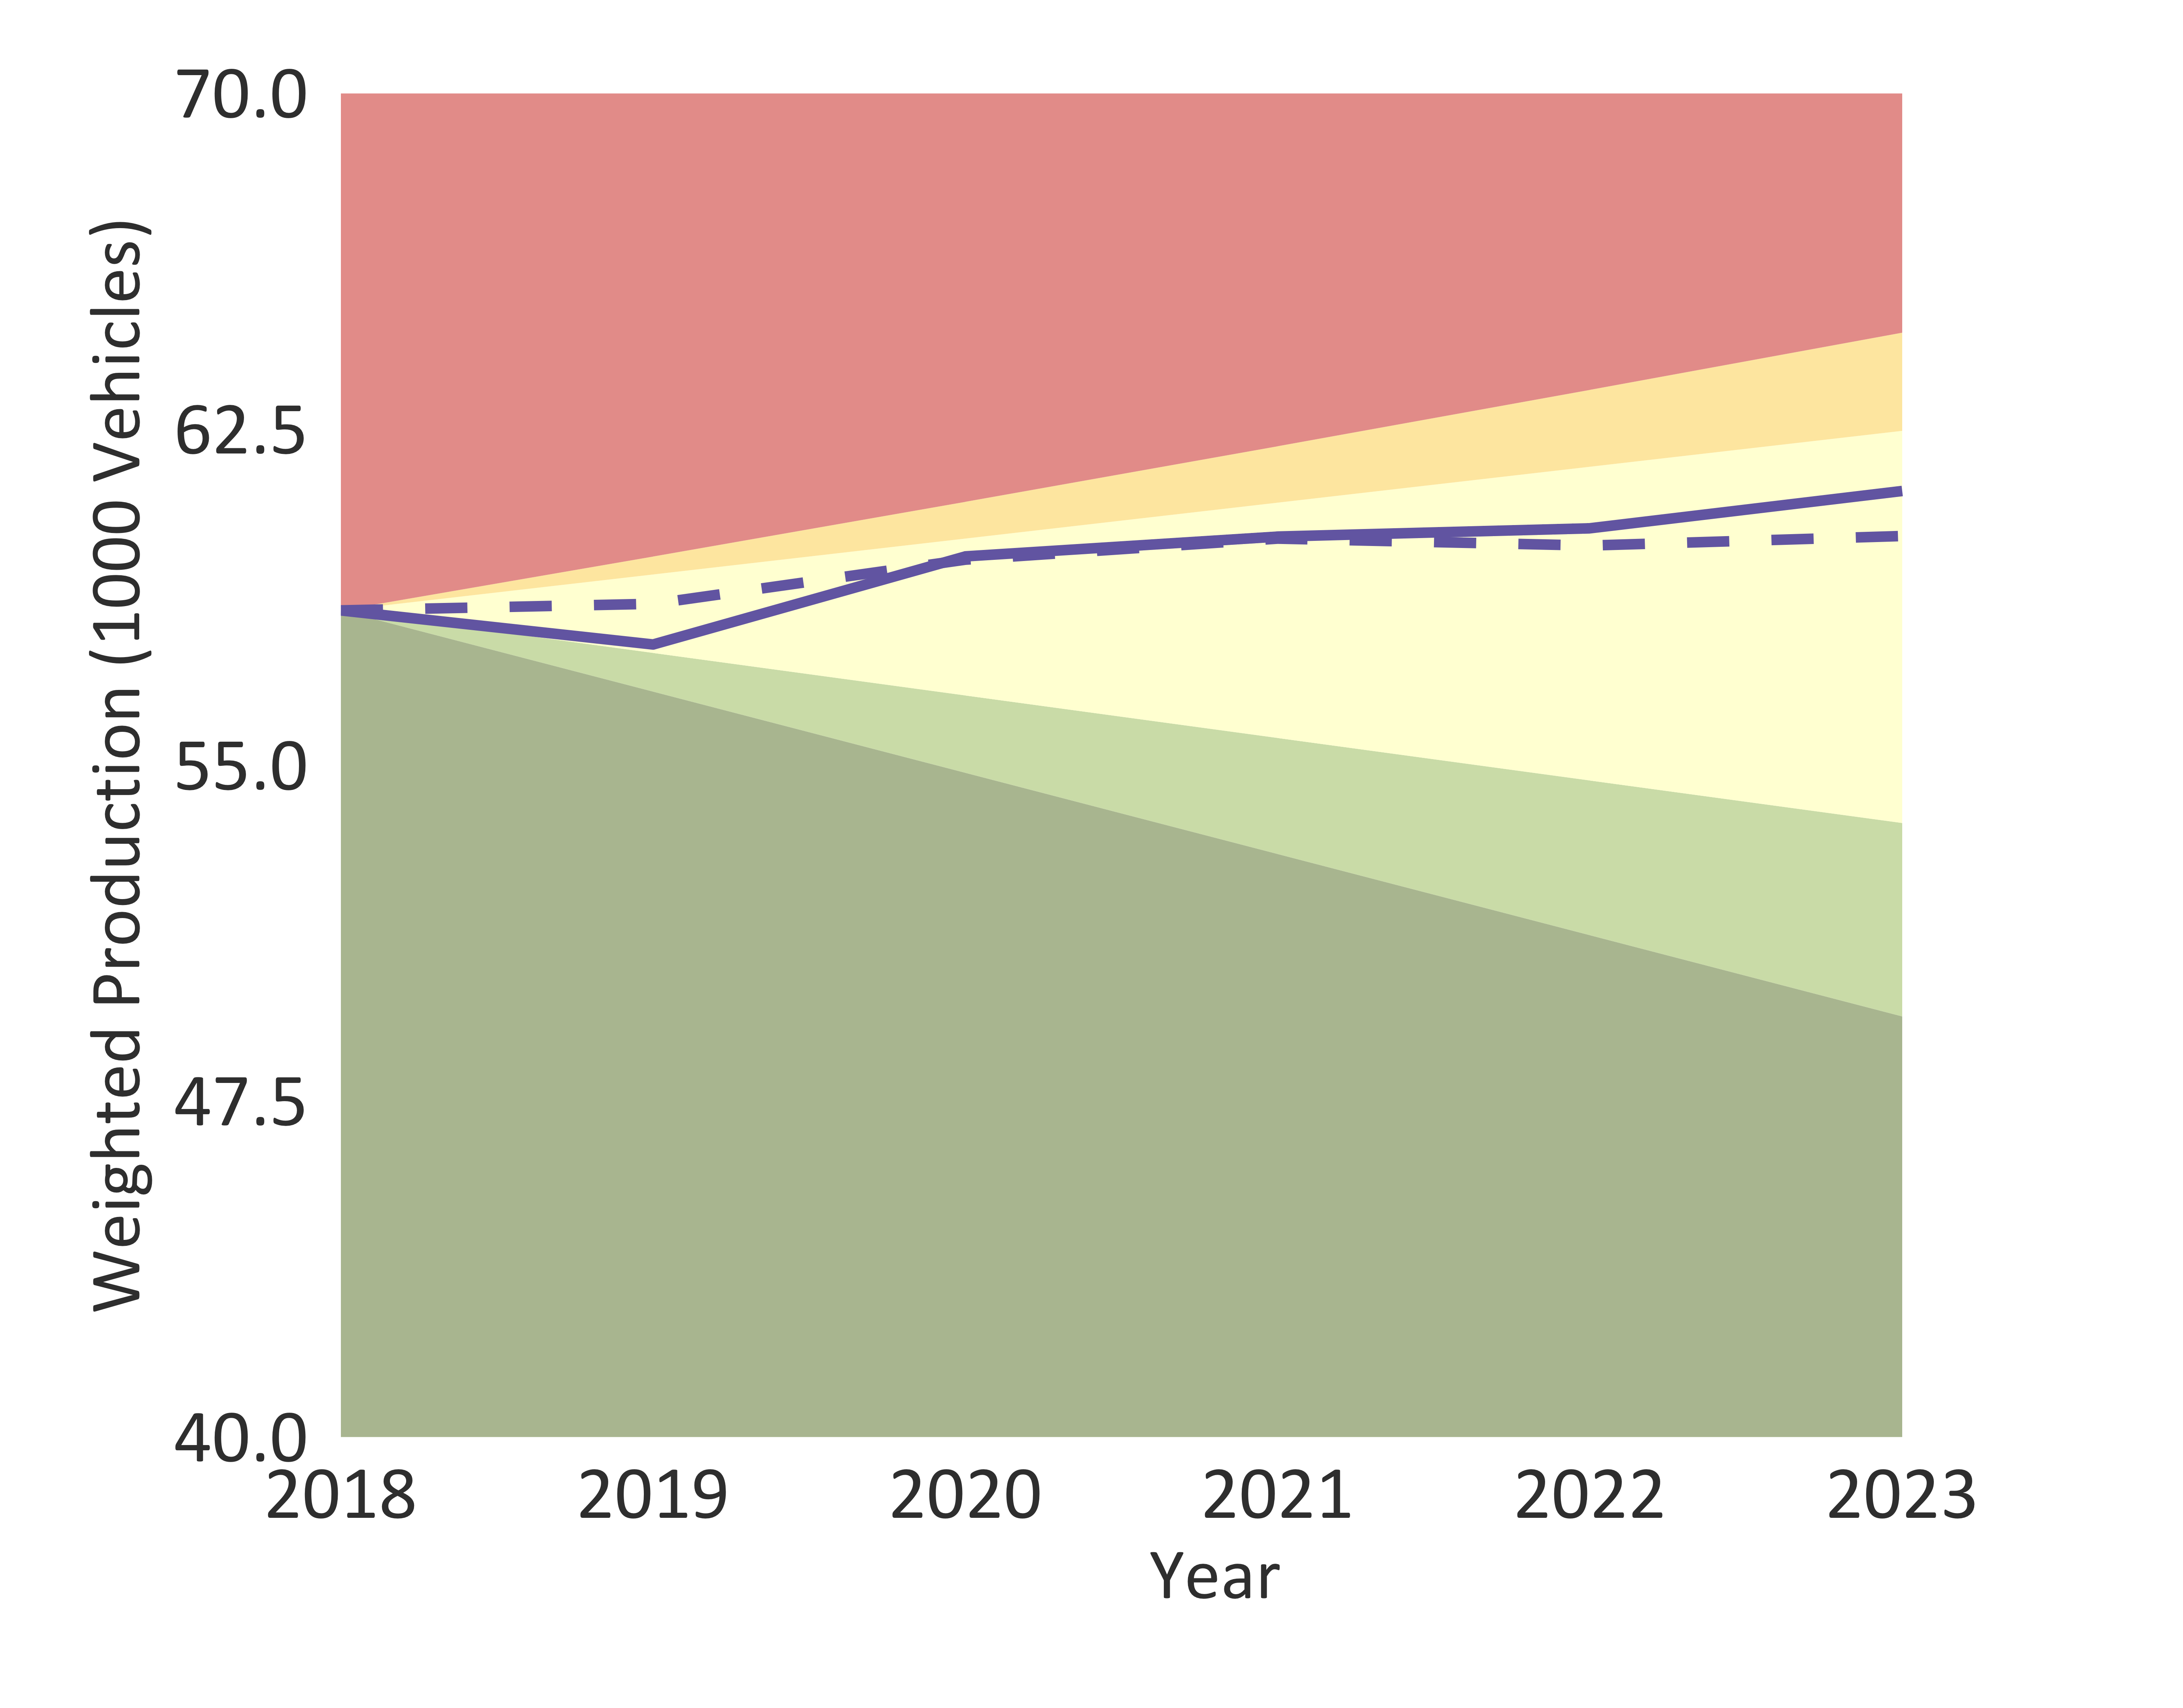
\includegraphics[trim = {0 0cm 0 0},width=1\linewidth]{CAFigures/Fig14}
		
		\textbf{Trajectory of Renewable Power Capacity }
		
		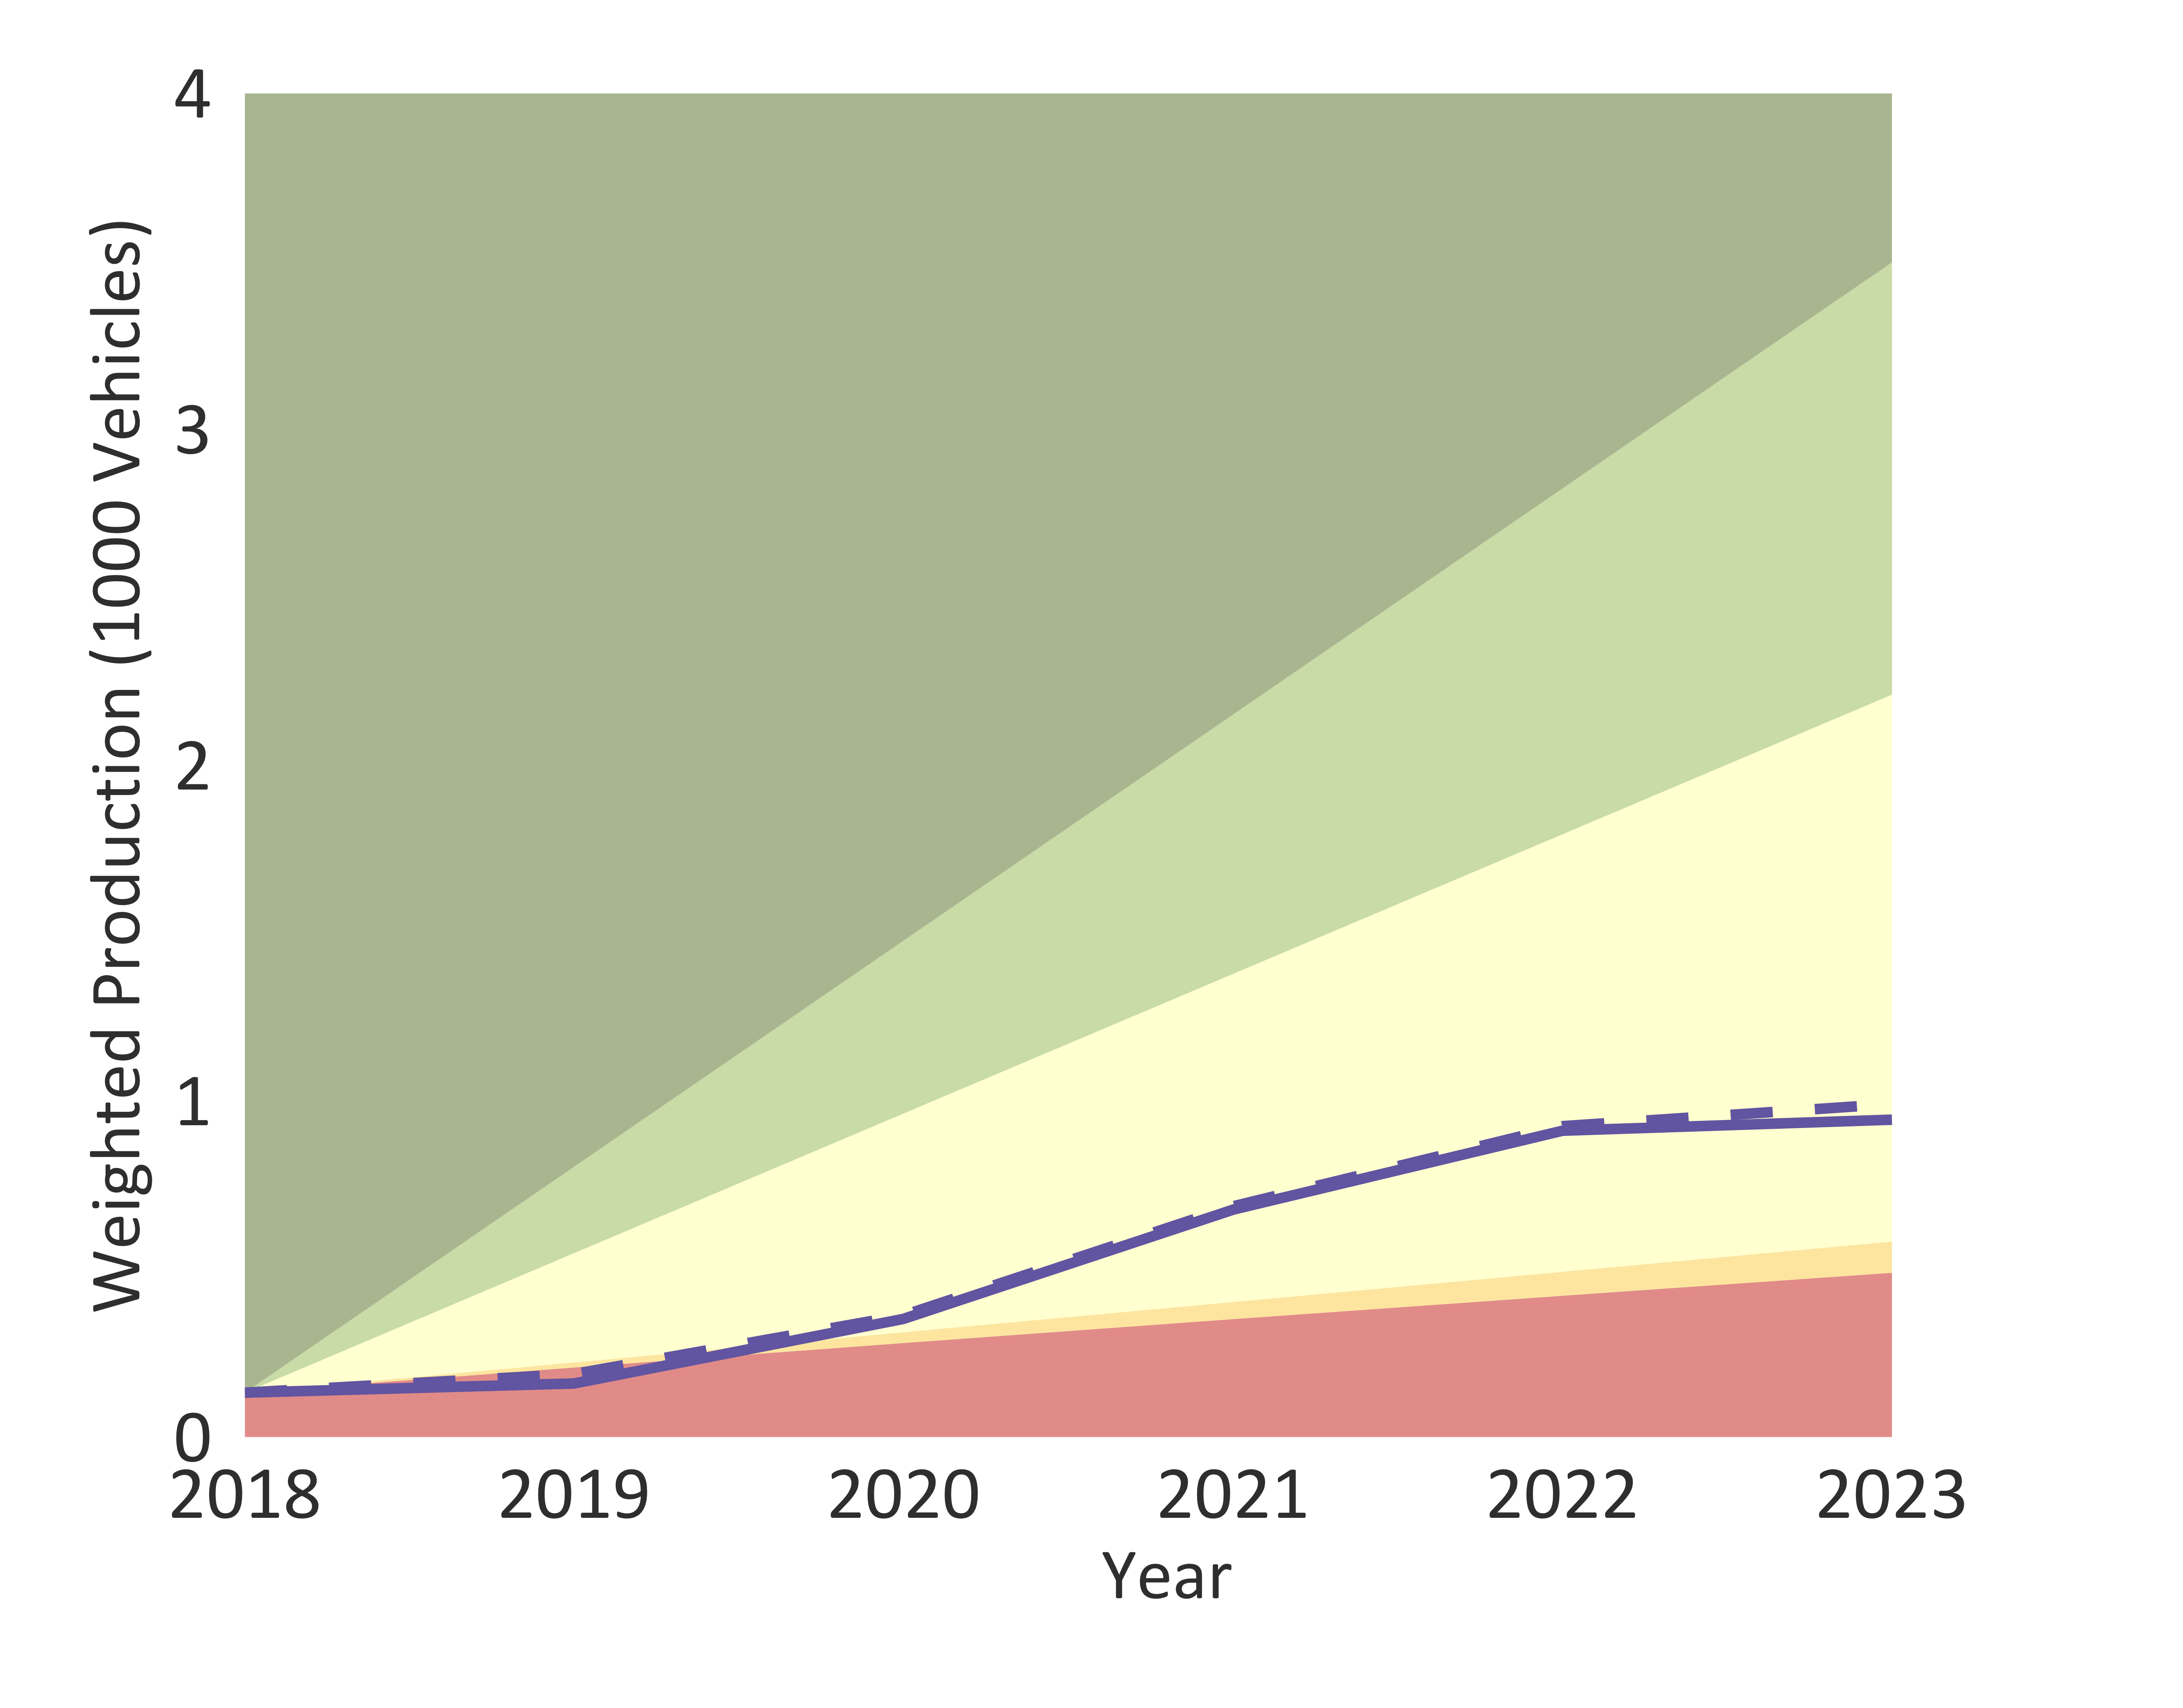
\includegraphics[trim = {0 0cm 0 0},width=.99\linewidth]{CAFigures/Fig15}
	\end{minipage}	
	\hspace{.02\linewidth}
	\begin{minipage}[t]{.49\textwidth}
		\textbf{Trajectory of Gas Power Capacity }
		
		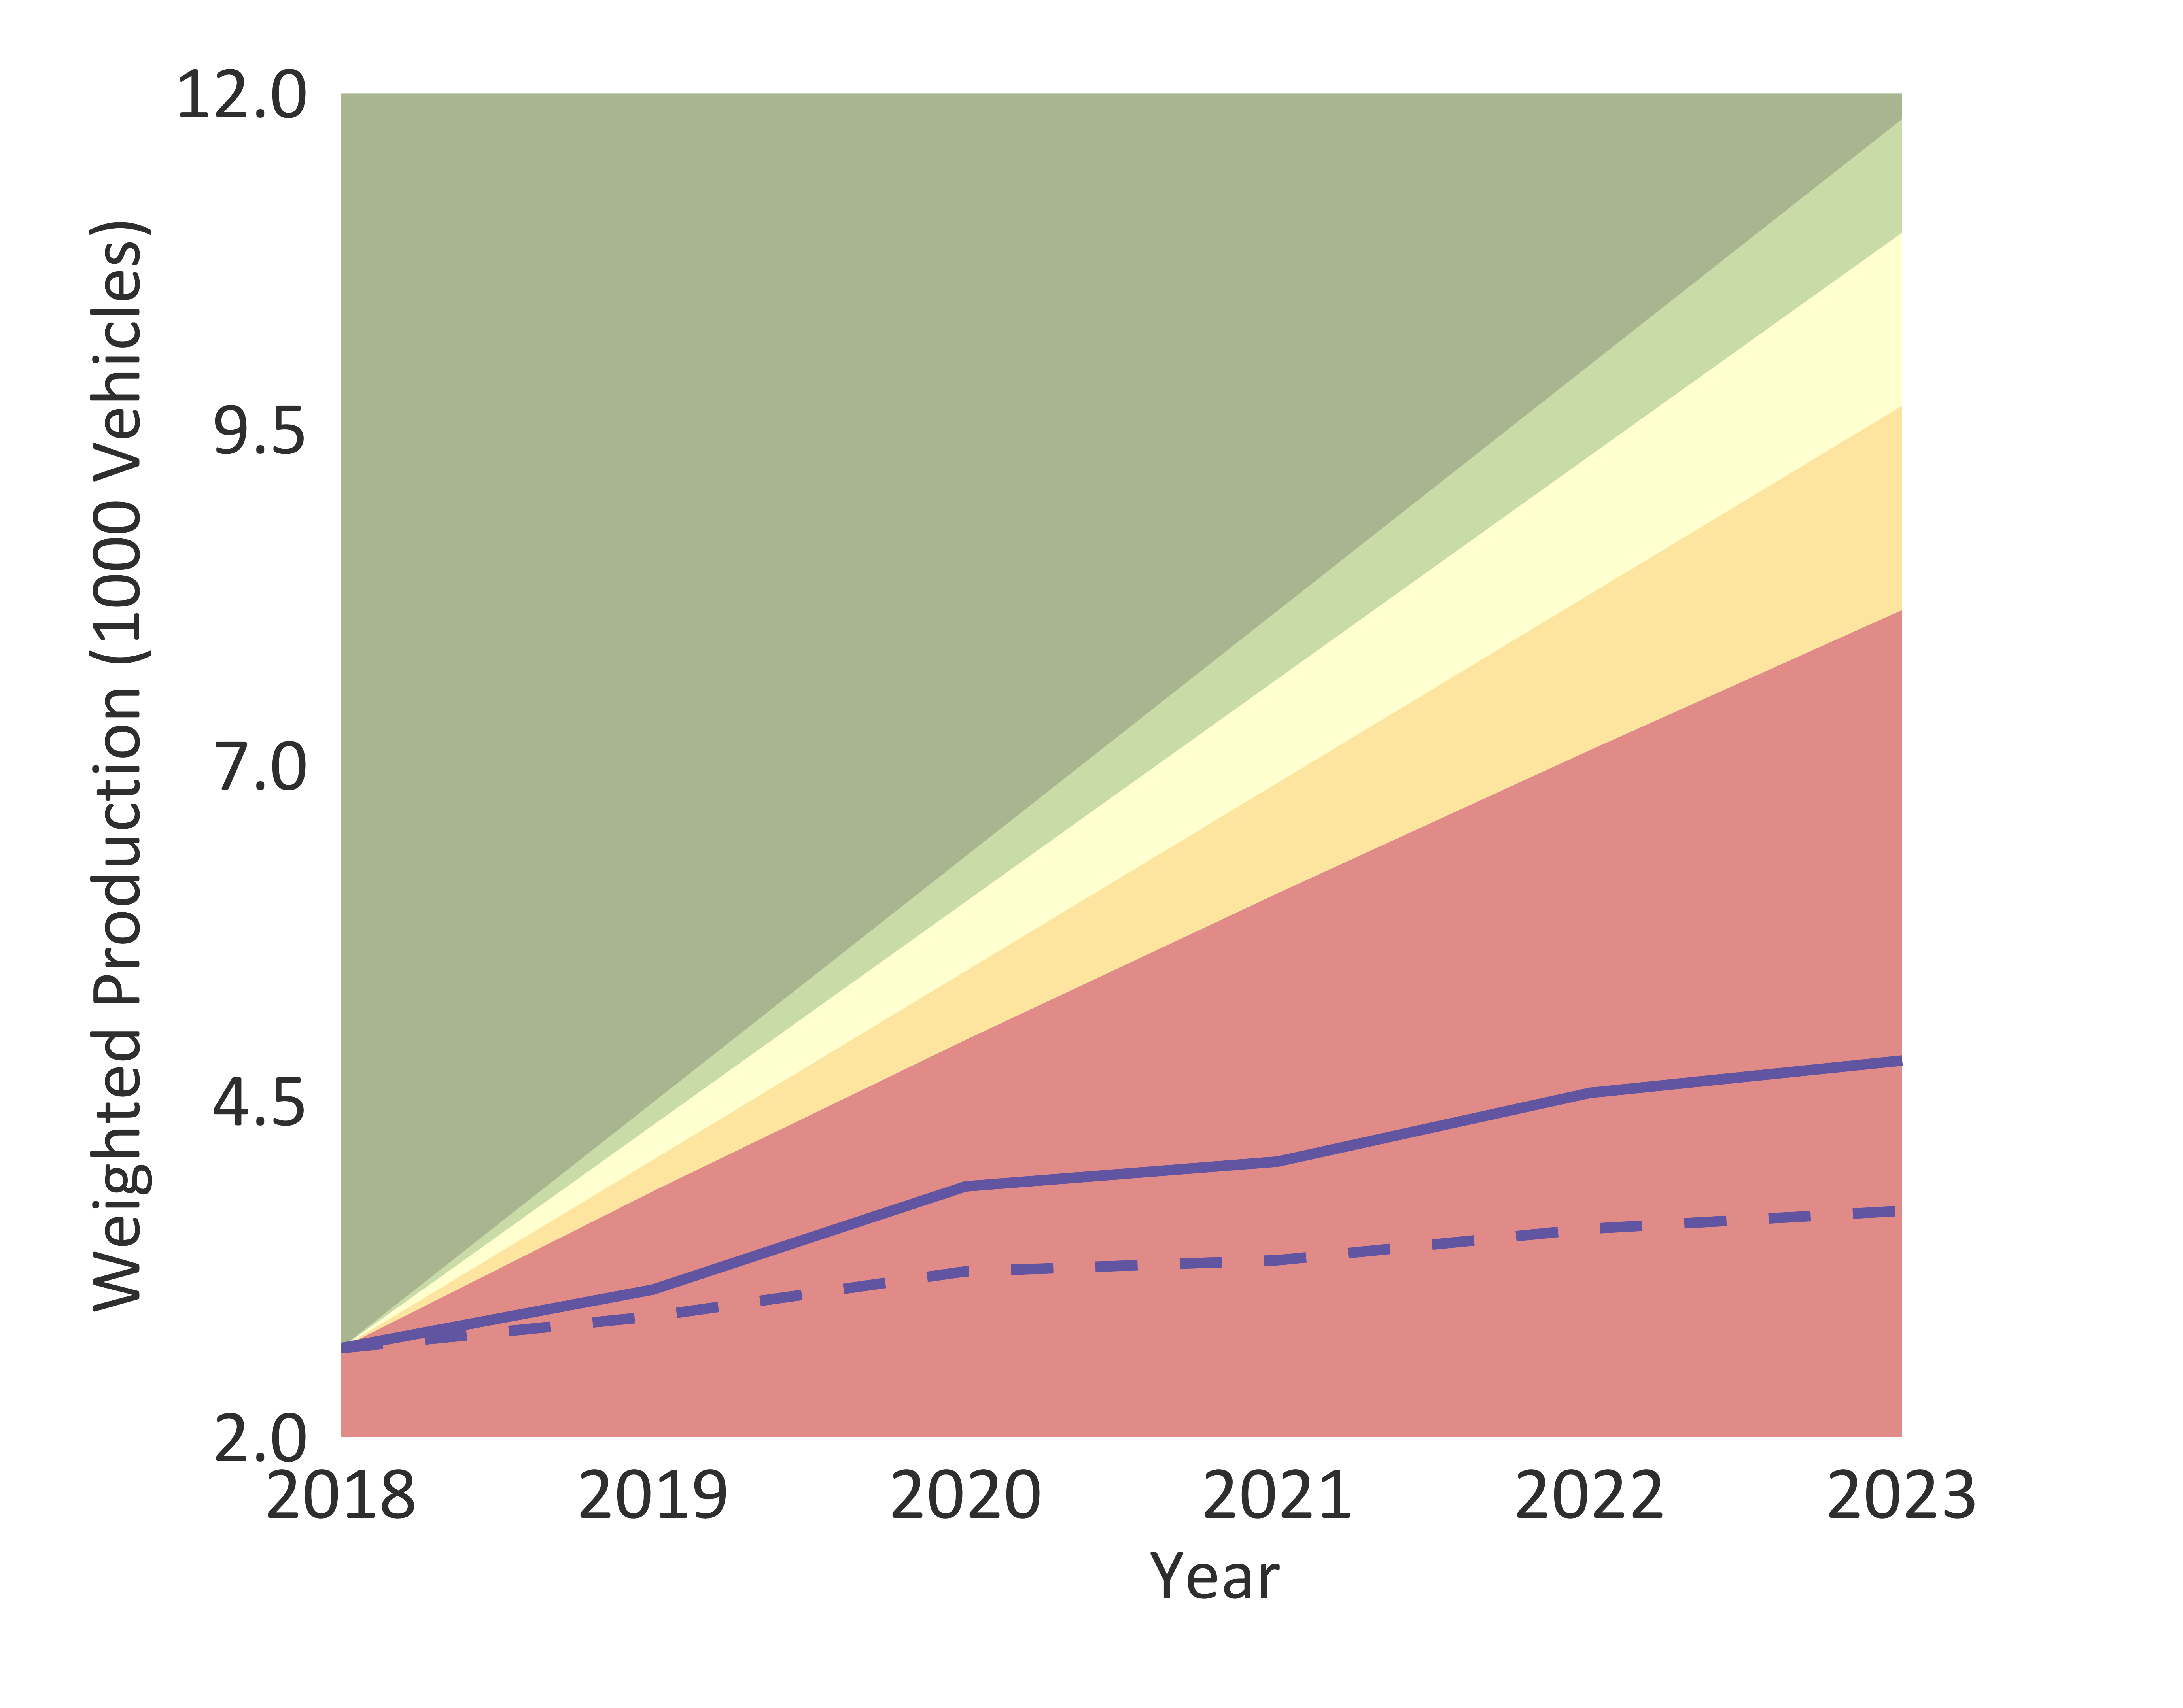
\includegraphics[trim = {0 0cm 0 0},width=1\linewidth]{CAFigures/Fig16}
		
		\textbf{Trajectory of Nuclear Power Capacity }
		
		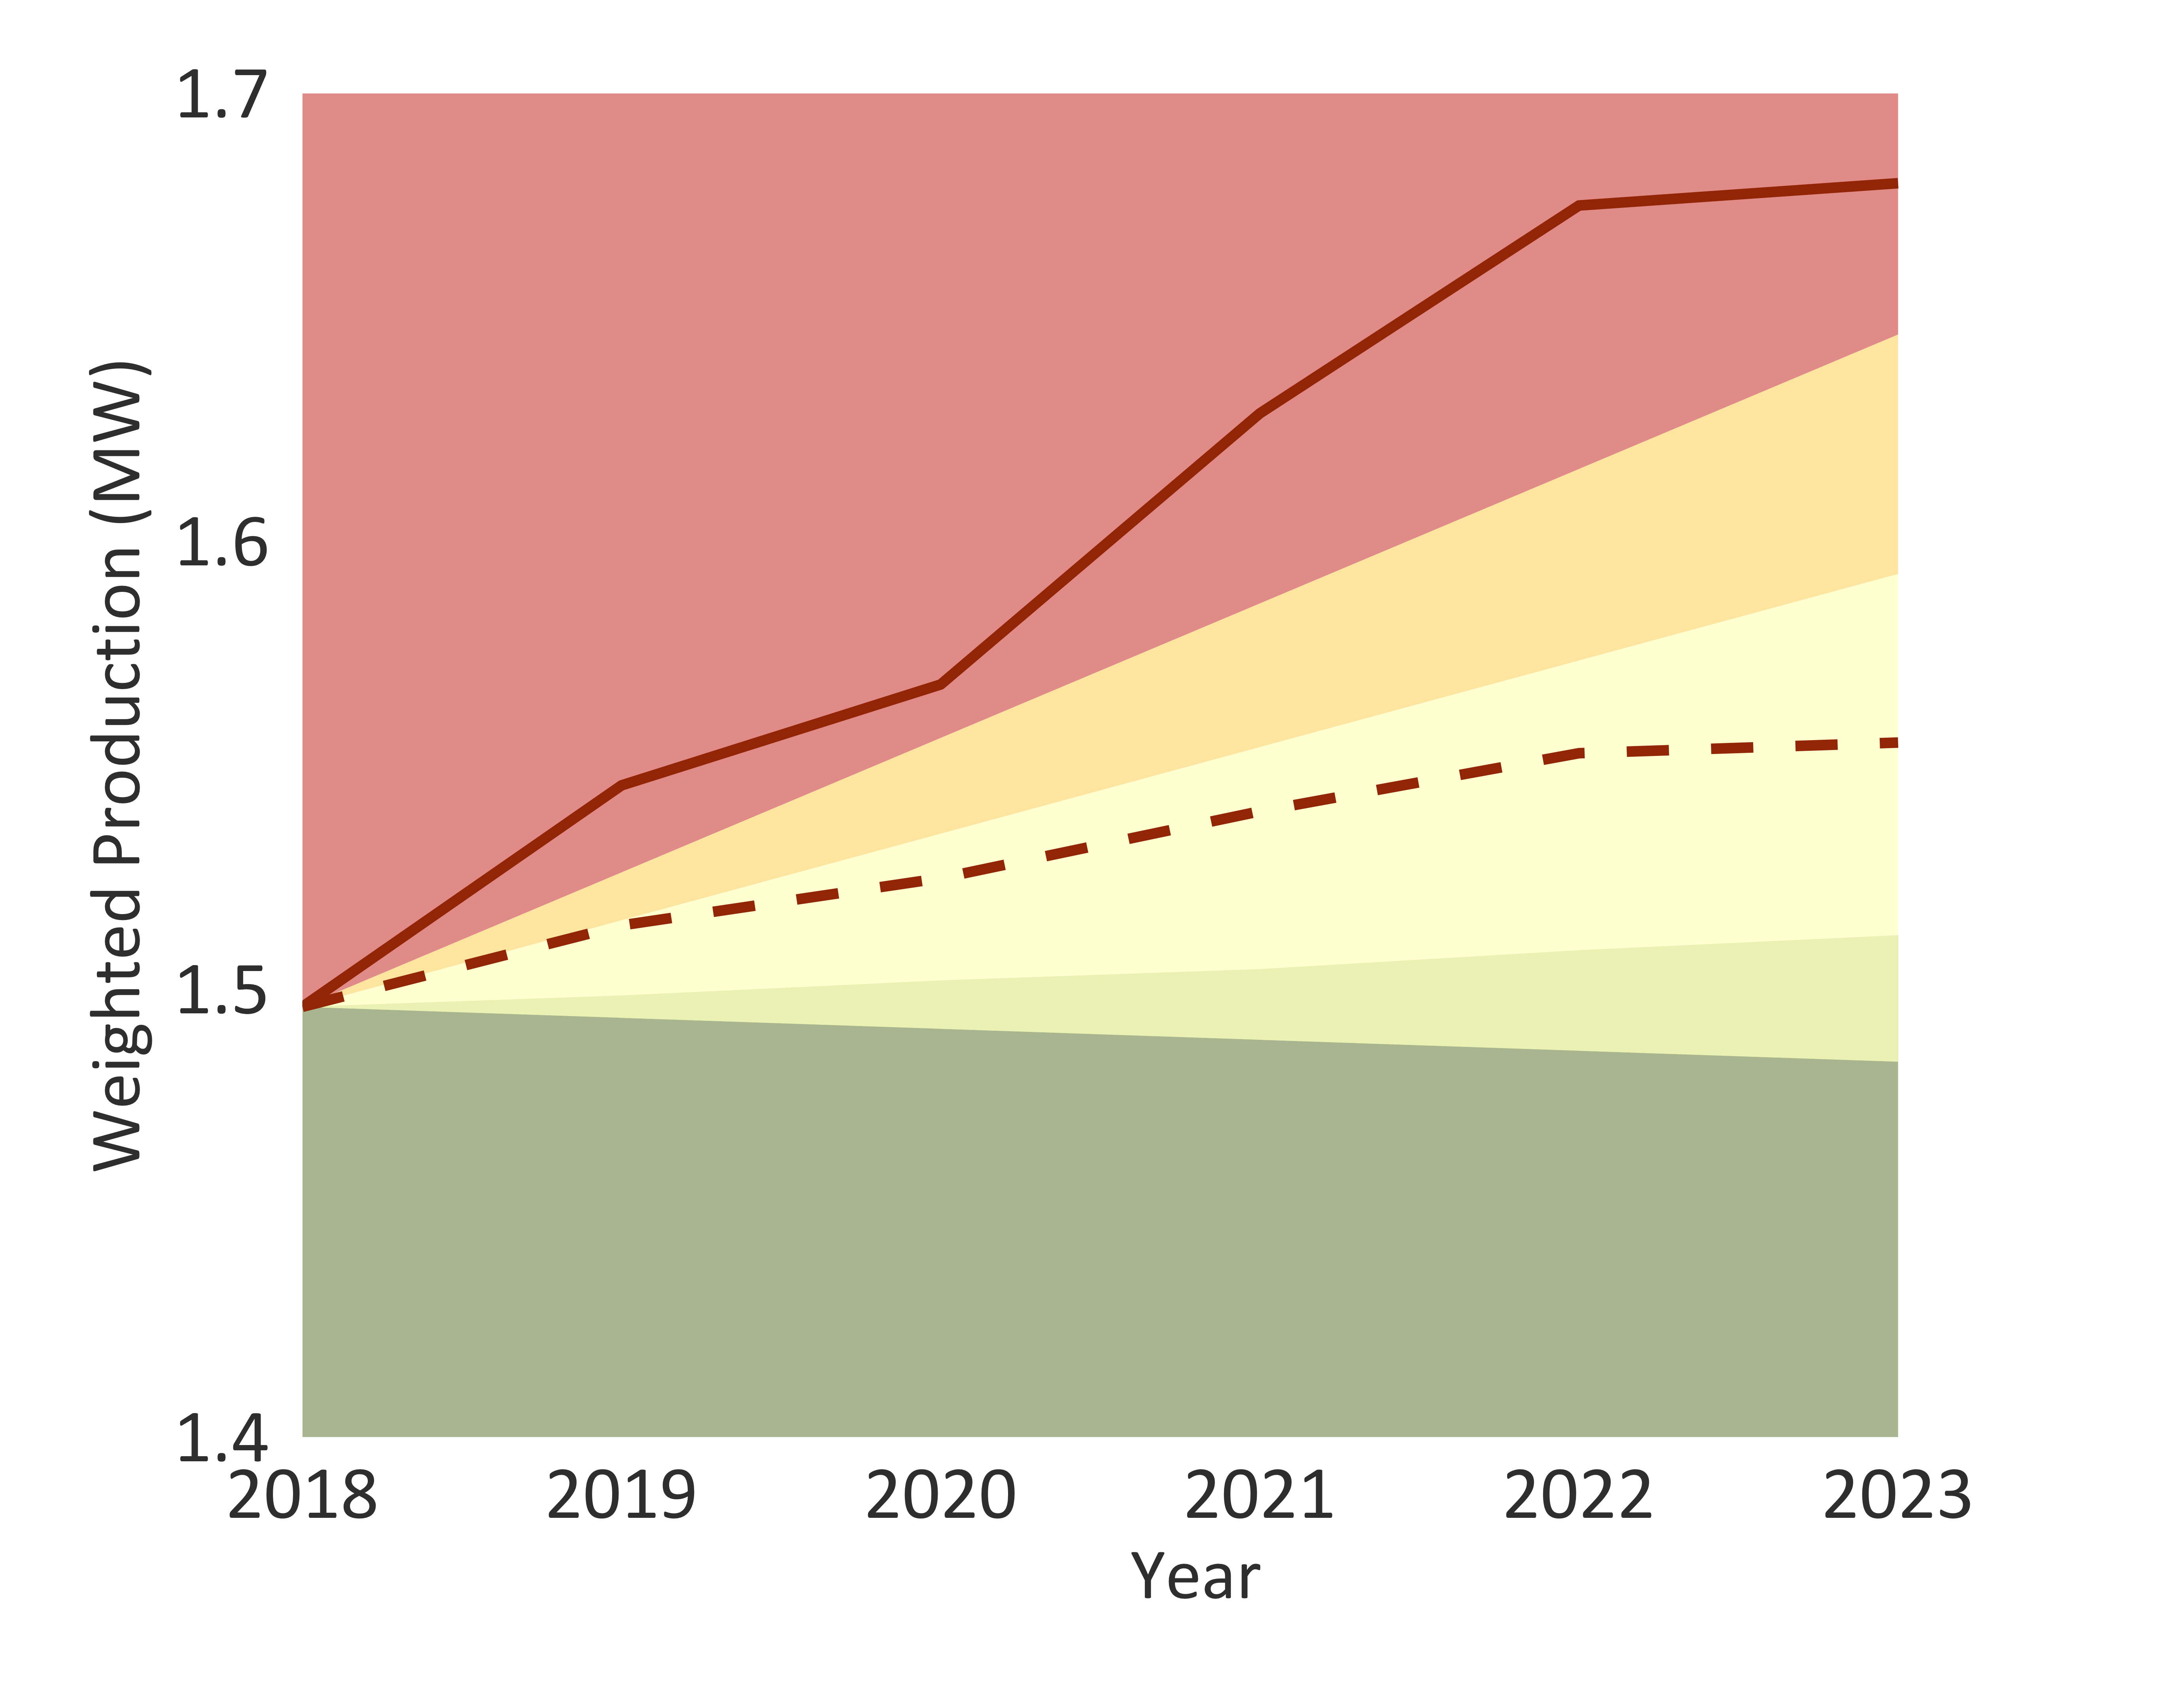
\includegraphics[trim = {0 0cm 0 0},width=1\linewidth]{CAFigures/Fig17}
		
	\end{minipage}
	
	\vspace{-0.4cm}
	\begin{center}
		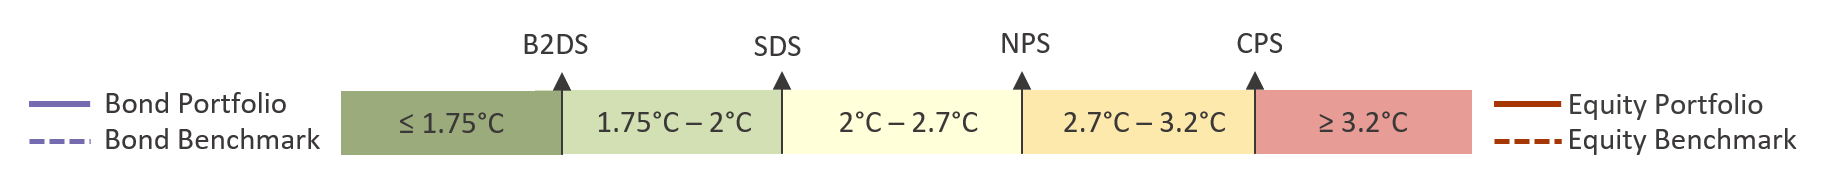
\includegraphics[trim = {0 0cm 0 0},width=.9\linewidth]{ReportGraphics/246Legend.png}
	\end{center}
	
	
	\PageFooterThird
	\newpage %CBSpecificE
	\section*{} % TRAJECTORY - EQUITY - POWER %EQSpecificS p15
	\HeaderDouble{5 YEAR TREND - EQUITY}{POWER}		
	
	\begin{multicols}{2}
		\textbf{The alignment graphs below show the alignment of selected power technologies in the equity portfolio relative to the IEA scenarios for 2°C, 4°C and 6°C temperature change and the global listed equity market.} 
		For each technology, the value plotted for the portfolio (solid line) is the planned evolution or `trajectory' of installed capacity allocated to the equity portfolio over the next 5 years. The lines separating the color-coded background areas plot the portfolio's `target production' for each technology under the 2°, 4°, and 6° scenarios. The dotted line shows the planned trajectory of installed capacity in the specific technology for the listed equity market, scaled to the same starting point as the portfolio.                    

	\end{multicols}
	
	
	
	\begin{minipage}[t]{.49\linewidth}
		\textbf{Trajectory of Coal Power Capacity }
		
		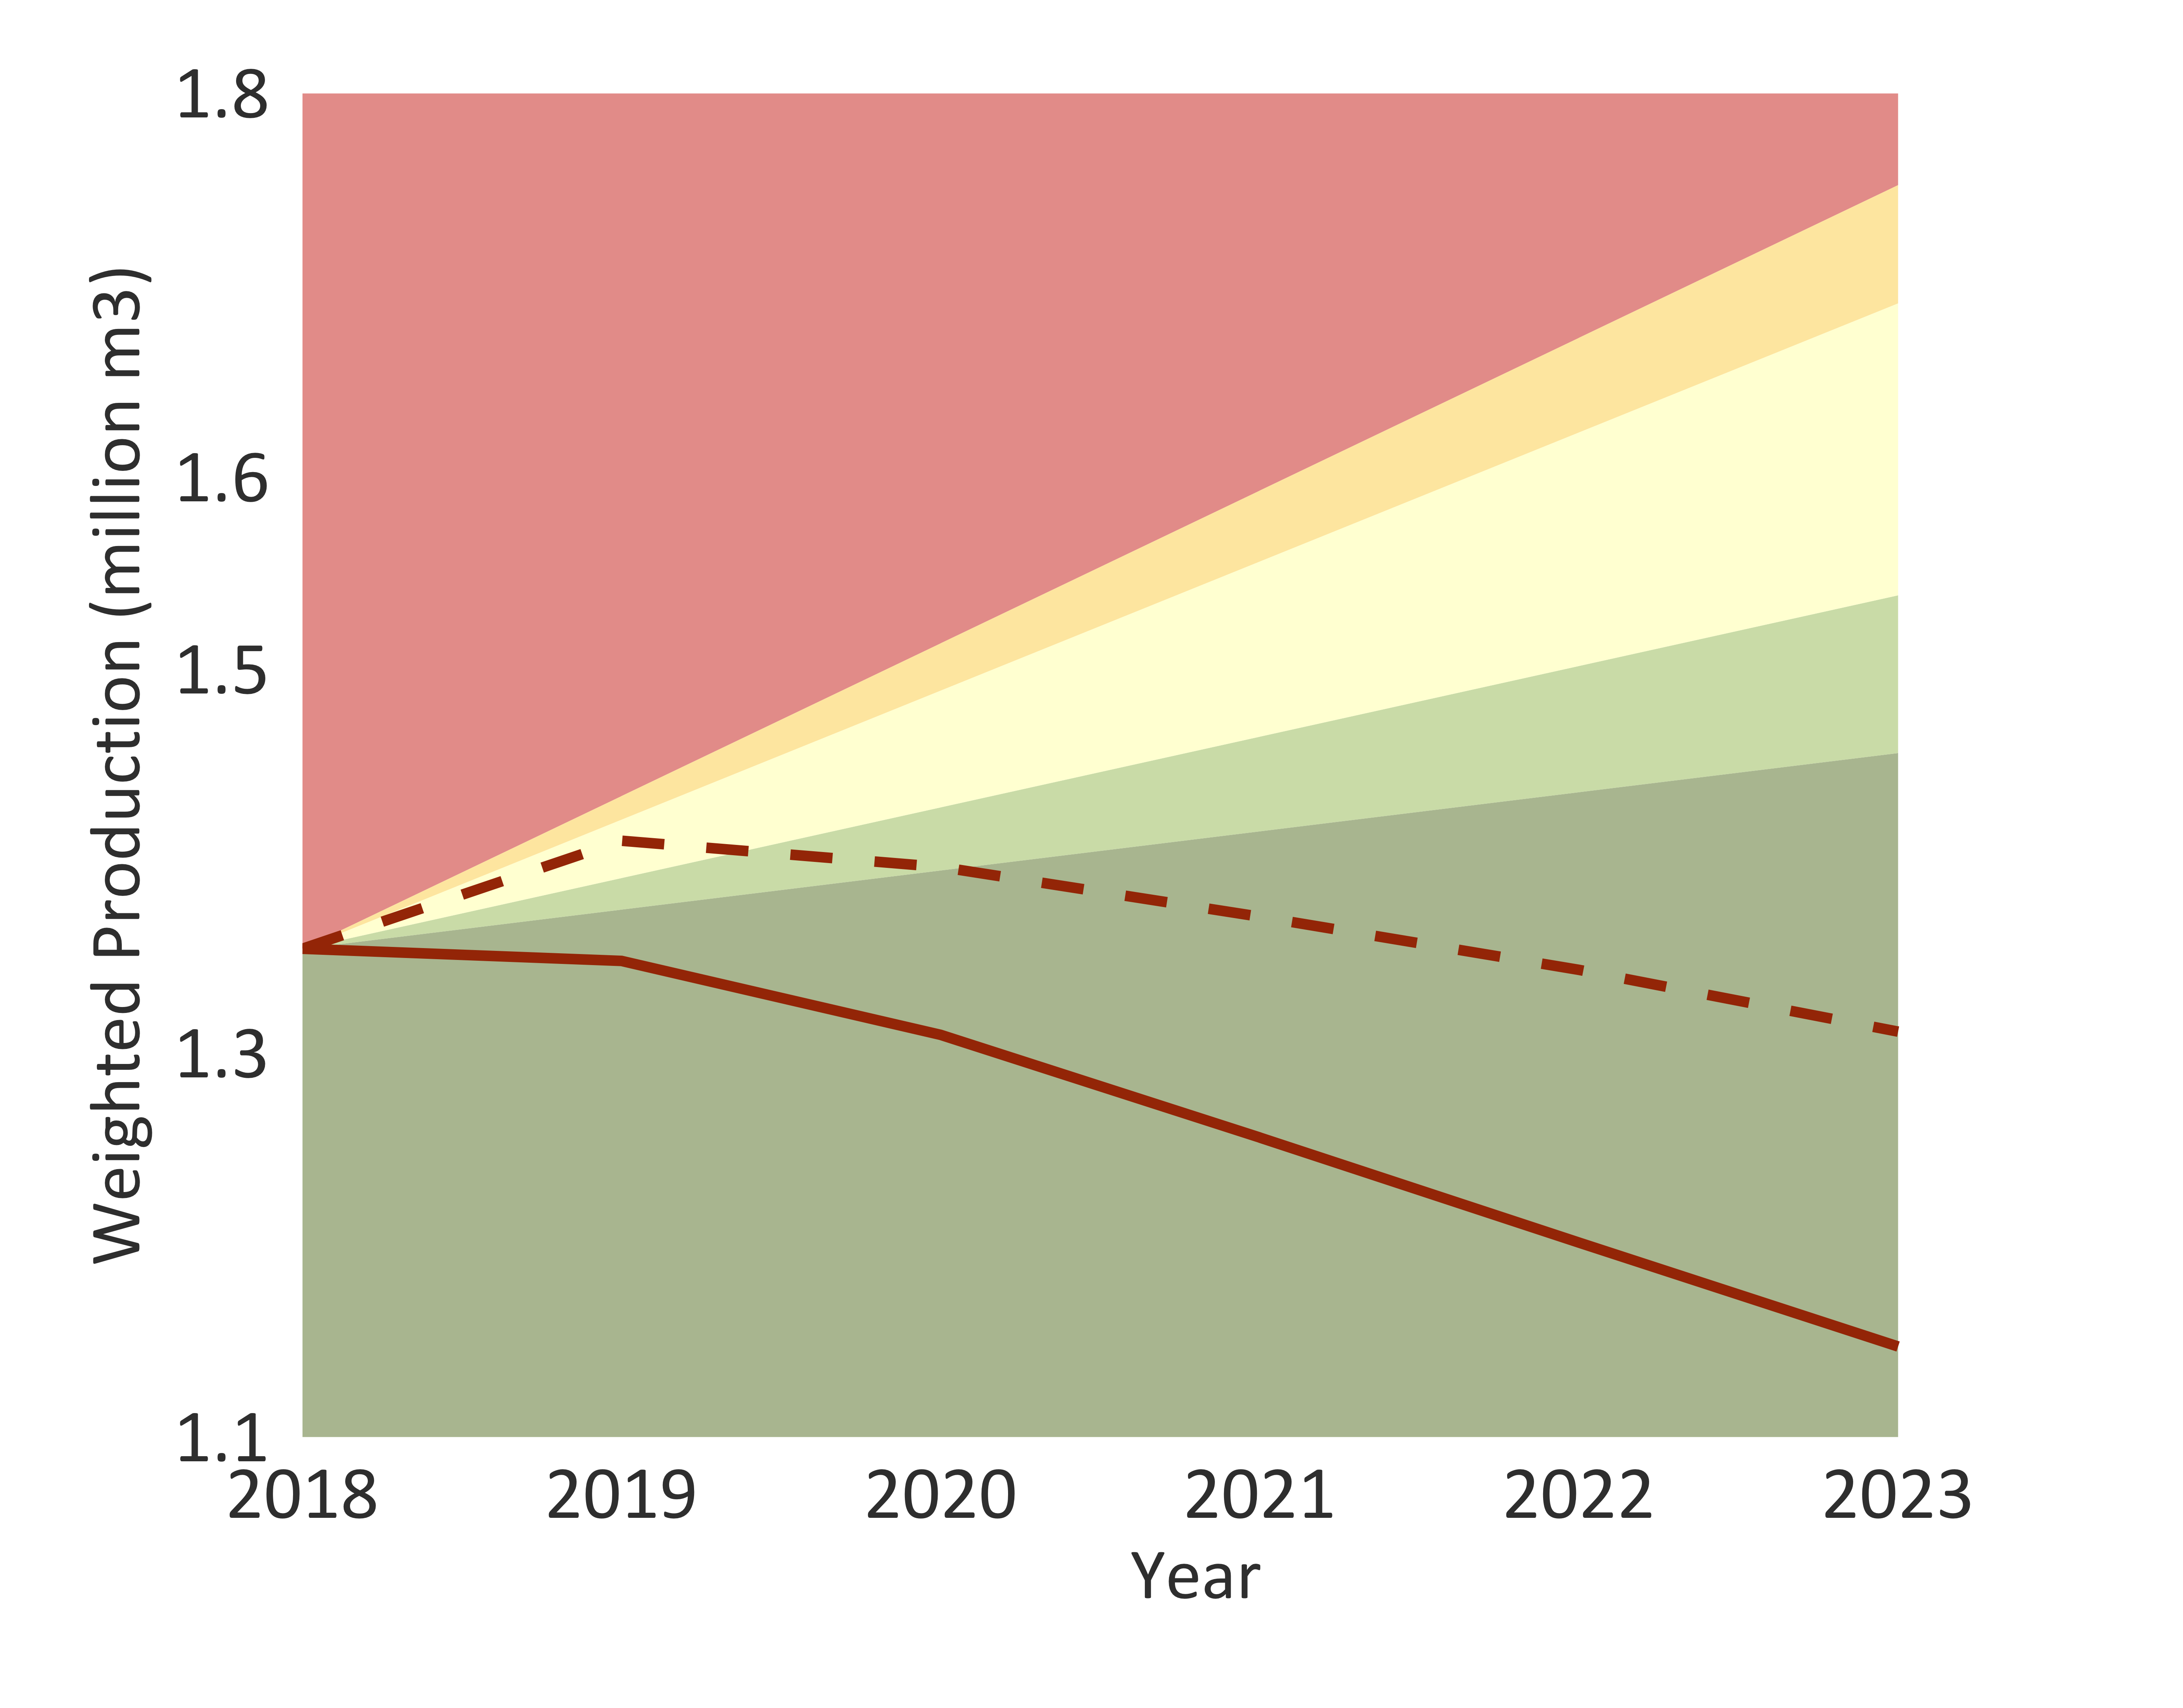
\includegraphics[trim = {0 0cm 0 0},width=1\linewidth]{CAFigures/Fig22}
		
		\textbf{Trajectory of Renewable Power Capacity }
		
		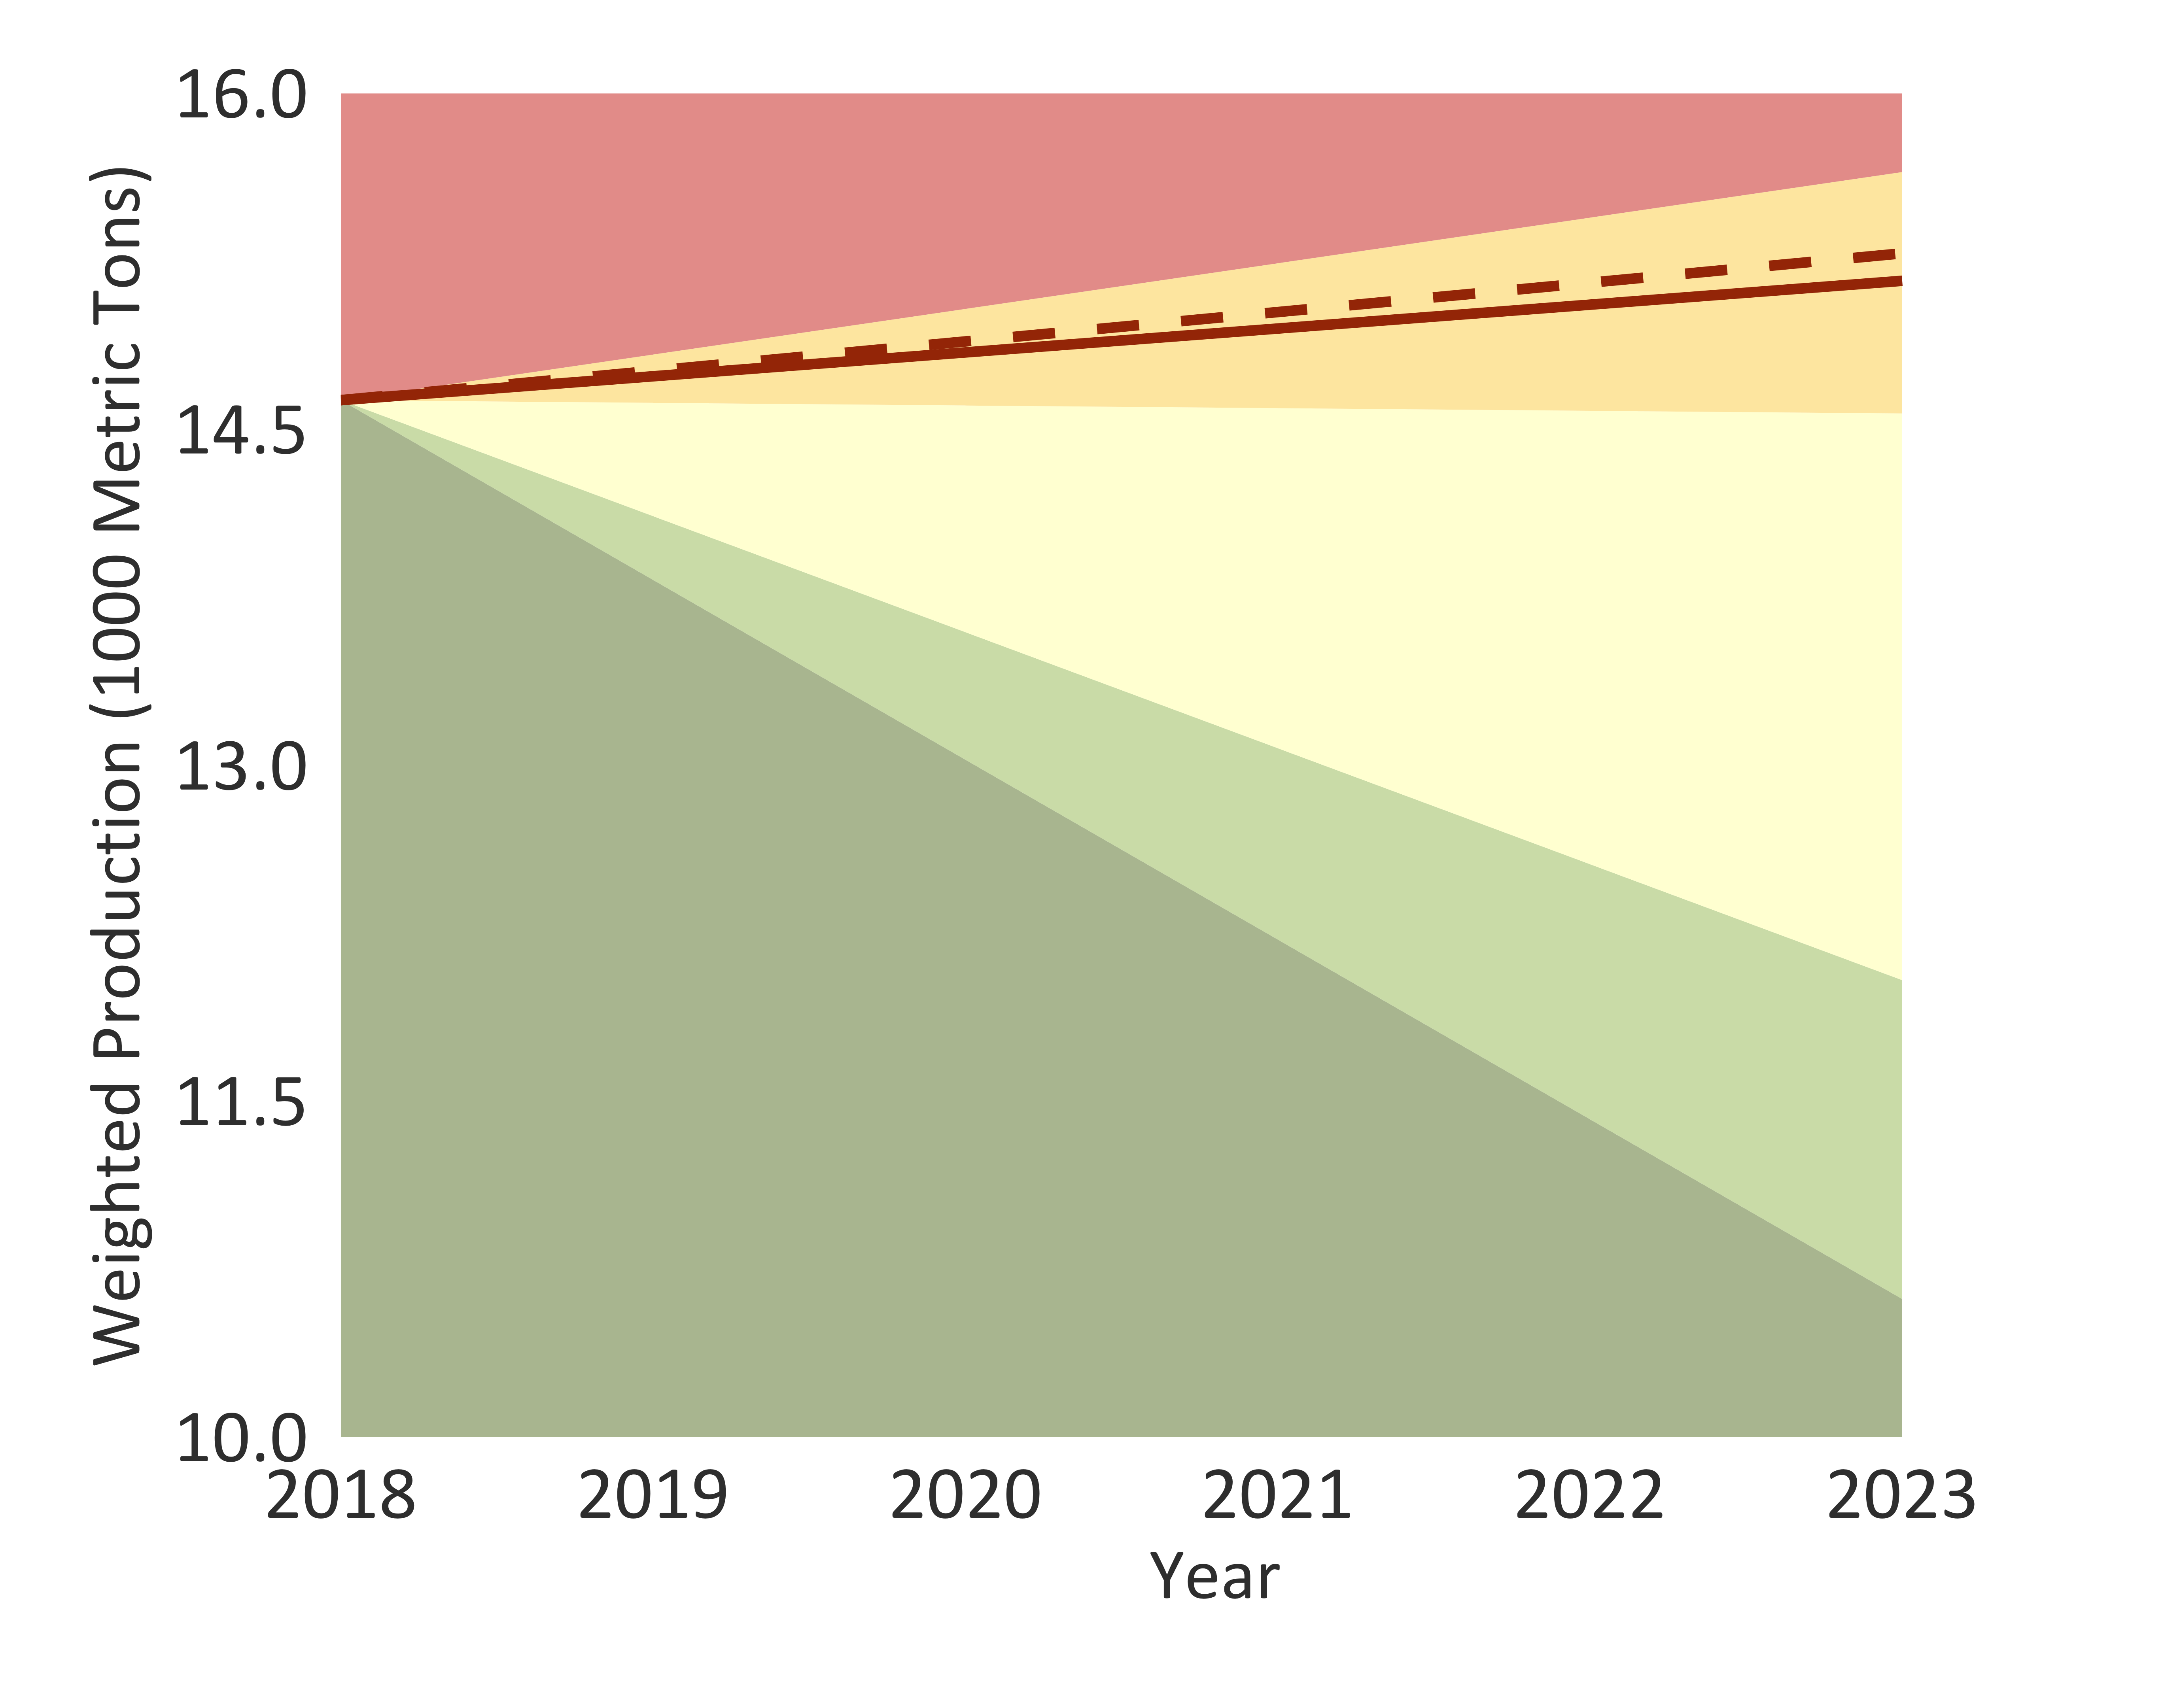
\includegraphics[trim = {0 0cm 0 0},width=.99\linewidth]{CAFigures/Fig23}
	\end{minipage}	
	\hspace{.02\linewidth}
	\begin{minipage}[t]{.49\textwidth}
		\textbf{Trajectory of Gas Power Capacity }
		
		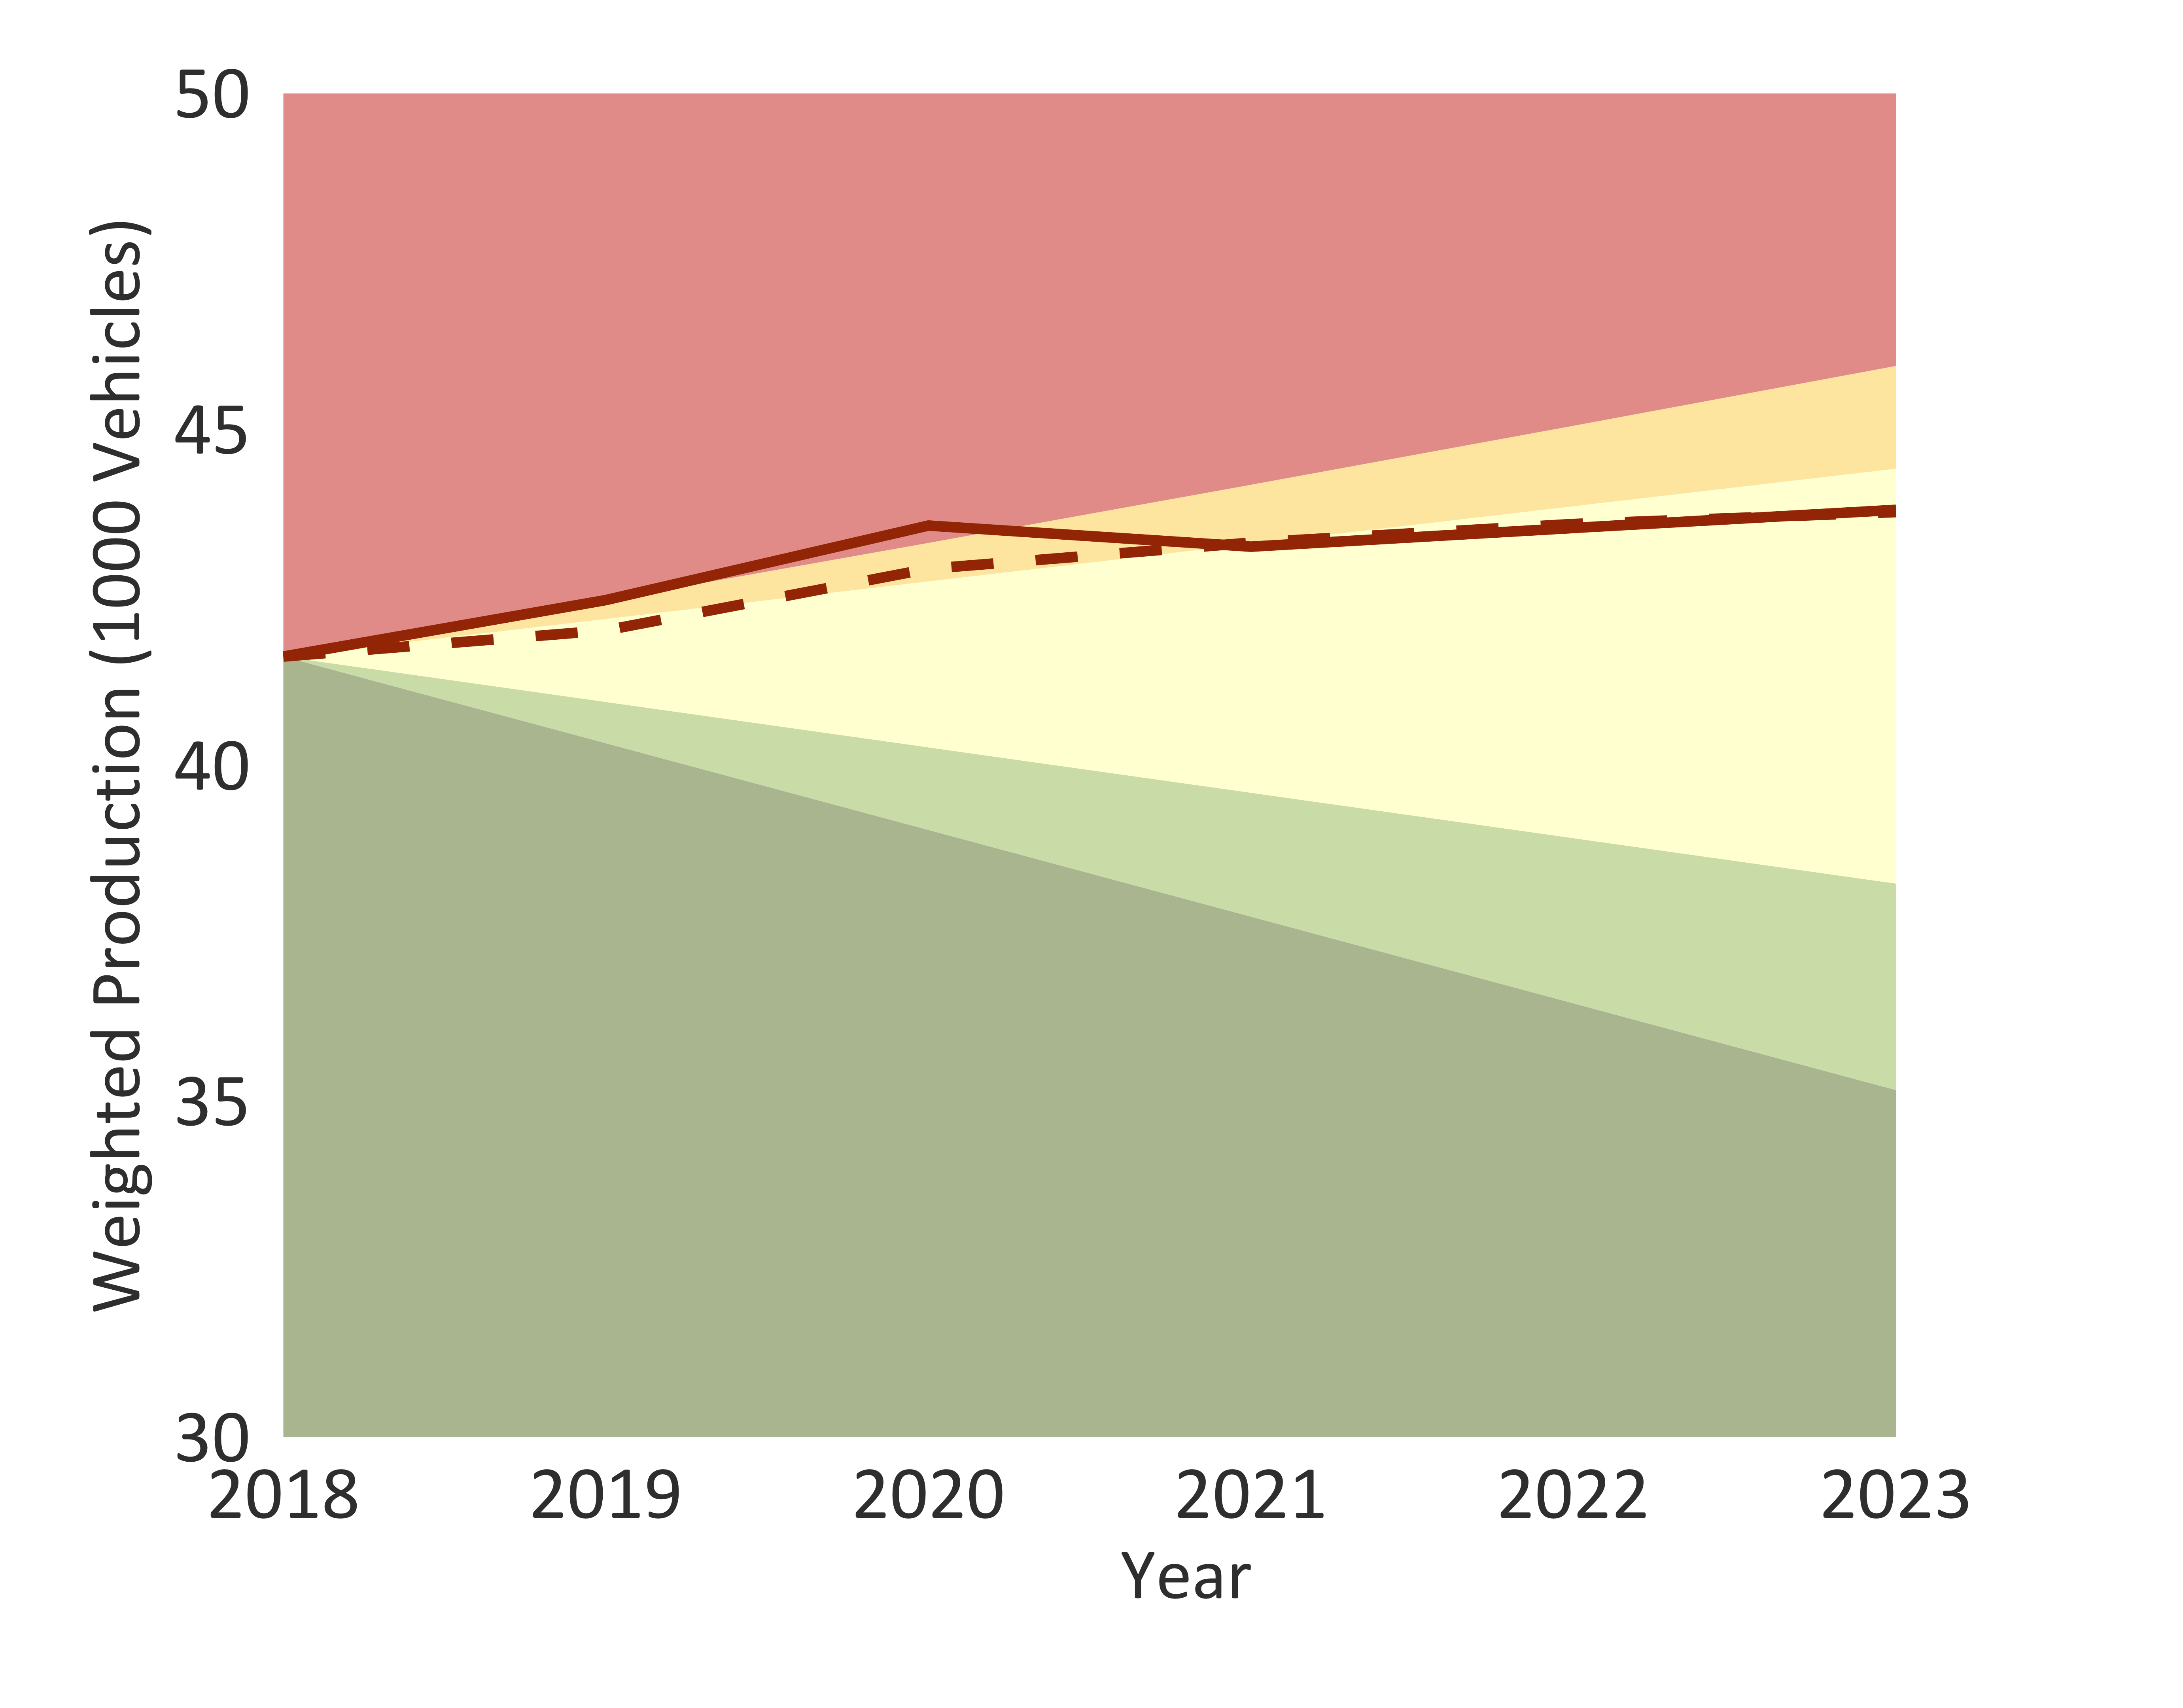
\includegraphics[trim = {0 0cm 0 0},width=1\linewidth]{CAFigures/Fig24}
		
		\textbf{Trajectory of Nuclear Power Capacity }
		
		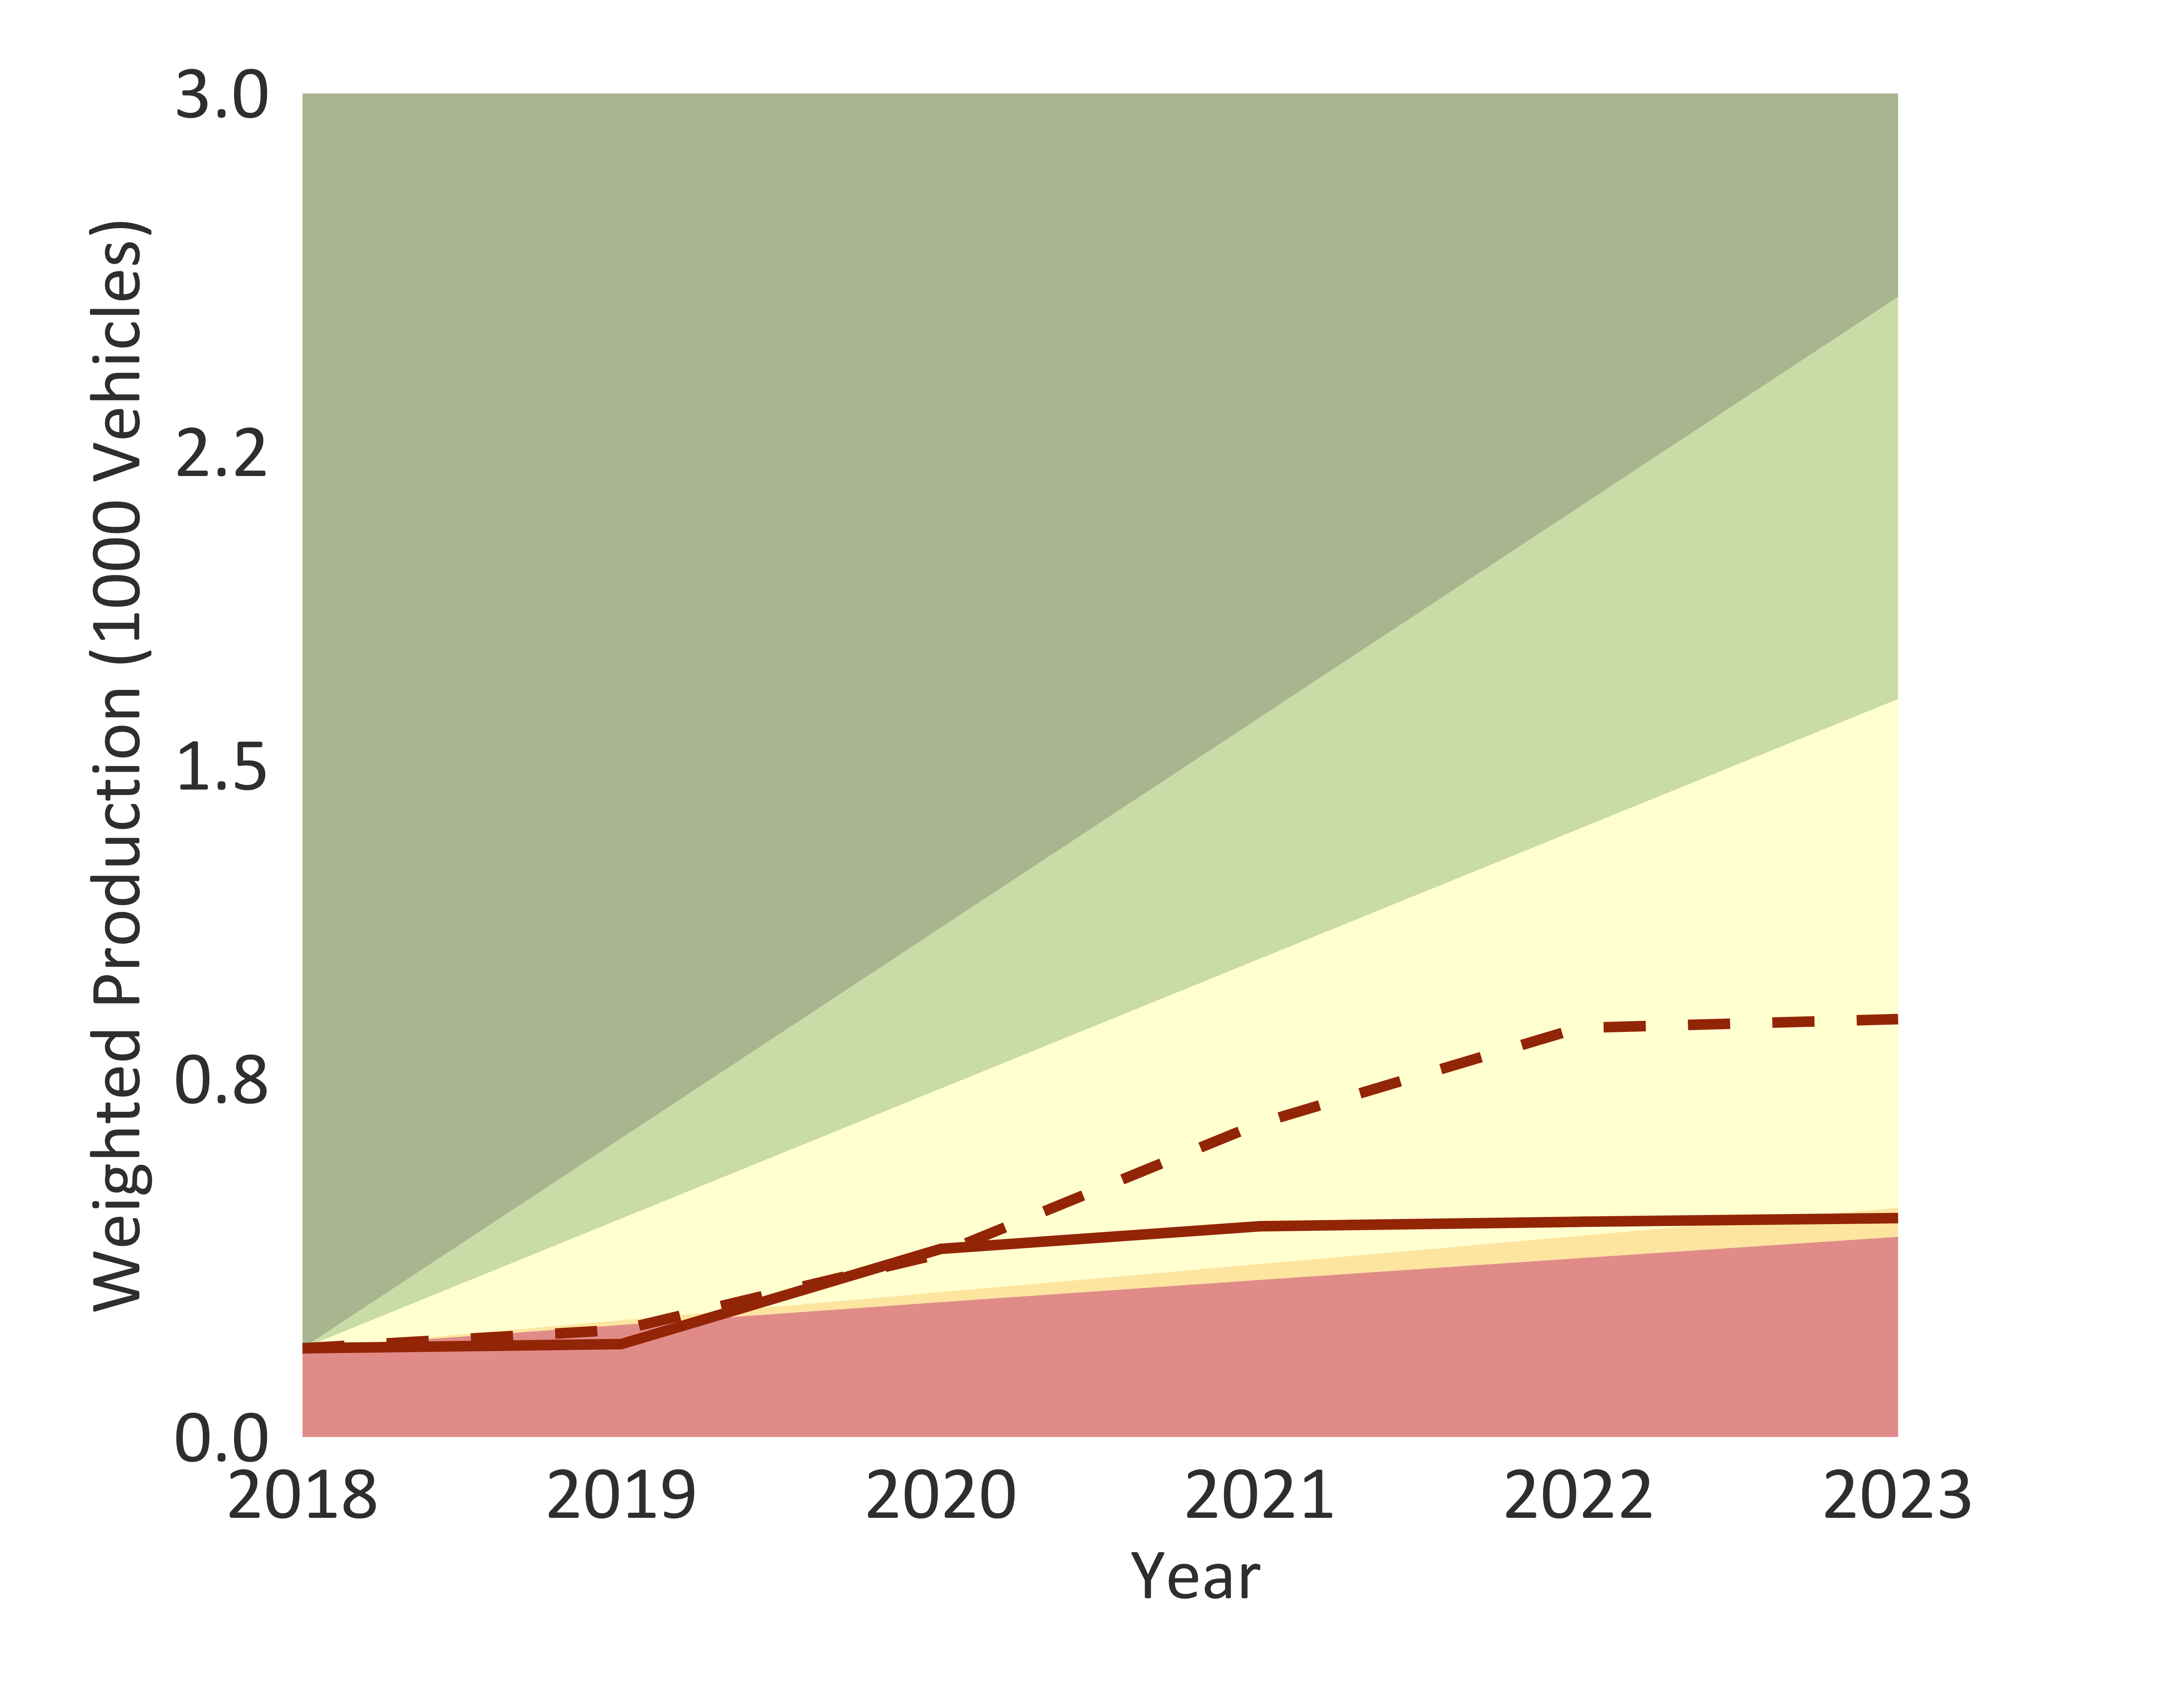
\includegraphics[trim = {0 0cm 0 0},width=1\linewidth]{CAFigures/Fig25}
		
	\end{minipage}
	
	\vspace{-0.6cm}
	\begin{center}
		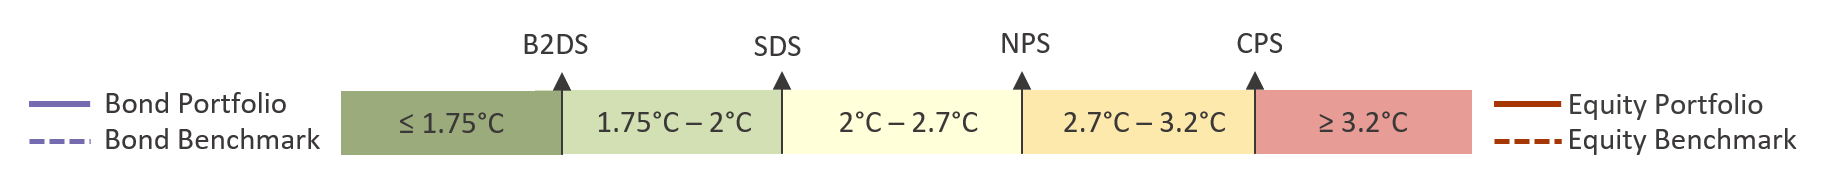
\includegraphics[trim = {0 0cm 0 0},width=.9\linewidth]{ReportGraphics/246Legend.png}
	\end{center}
	
	
	\PageFooterThird
	\newpage %EQSpecificE
	\section*{} % TRAJECTORY - FI - FOSSIL FUELS AND AUTOMOTIVE     %CBSpecificS p16
	\HeaderDouble{5 YEAR TREND - FIXED INCOME}{FOSSIL FUELS AND AUTOMOTIVE}	
	
	\begin{multicols}{2}
		\textbf{The alignment graphs below show the alignment of selected fossil fuels and automobile technologies in the fixed income portfolio relative to the IEA scenarios for 2°C, 4°C and 6°C temperature change. } 
		For each technology, the value plotted for the portfolio (solid line) is the planned evolution or `trajectory' of fossil fuel production (top graphs) or automobile production (bottom graphs) allocated to the fixed income portfolio over the next 5 years.  The lines separating the color-coded background areas plot the portfolio's 'target production' for each technology under the 2°, 4°, and 6° scenarios. The dotted line shows planned production in the specific technology for the fixed income market, scaled to the same starting point as the portfolio.                    

		
	\end{multicols}		
	
	\begin{center}
		\textbf{Fossil Fuel Sector}
	\end{center}
	
	\begin{minipage}[t]{.49\linewidth}
		\textbf{Trajectory of Oil Production }
		
		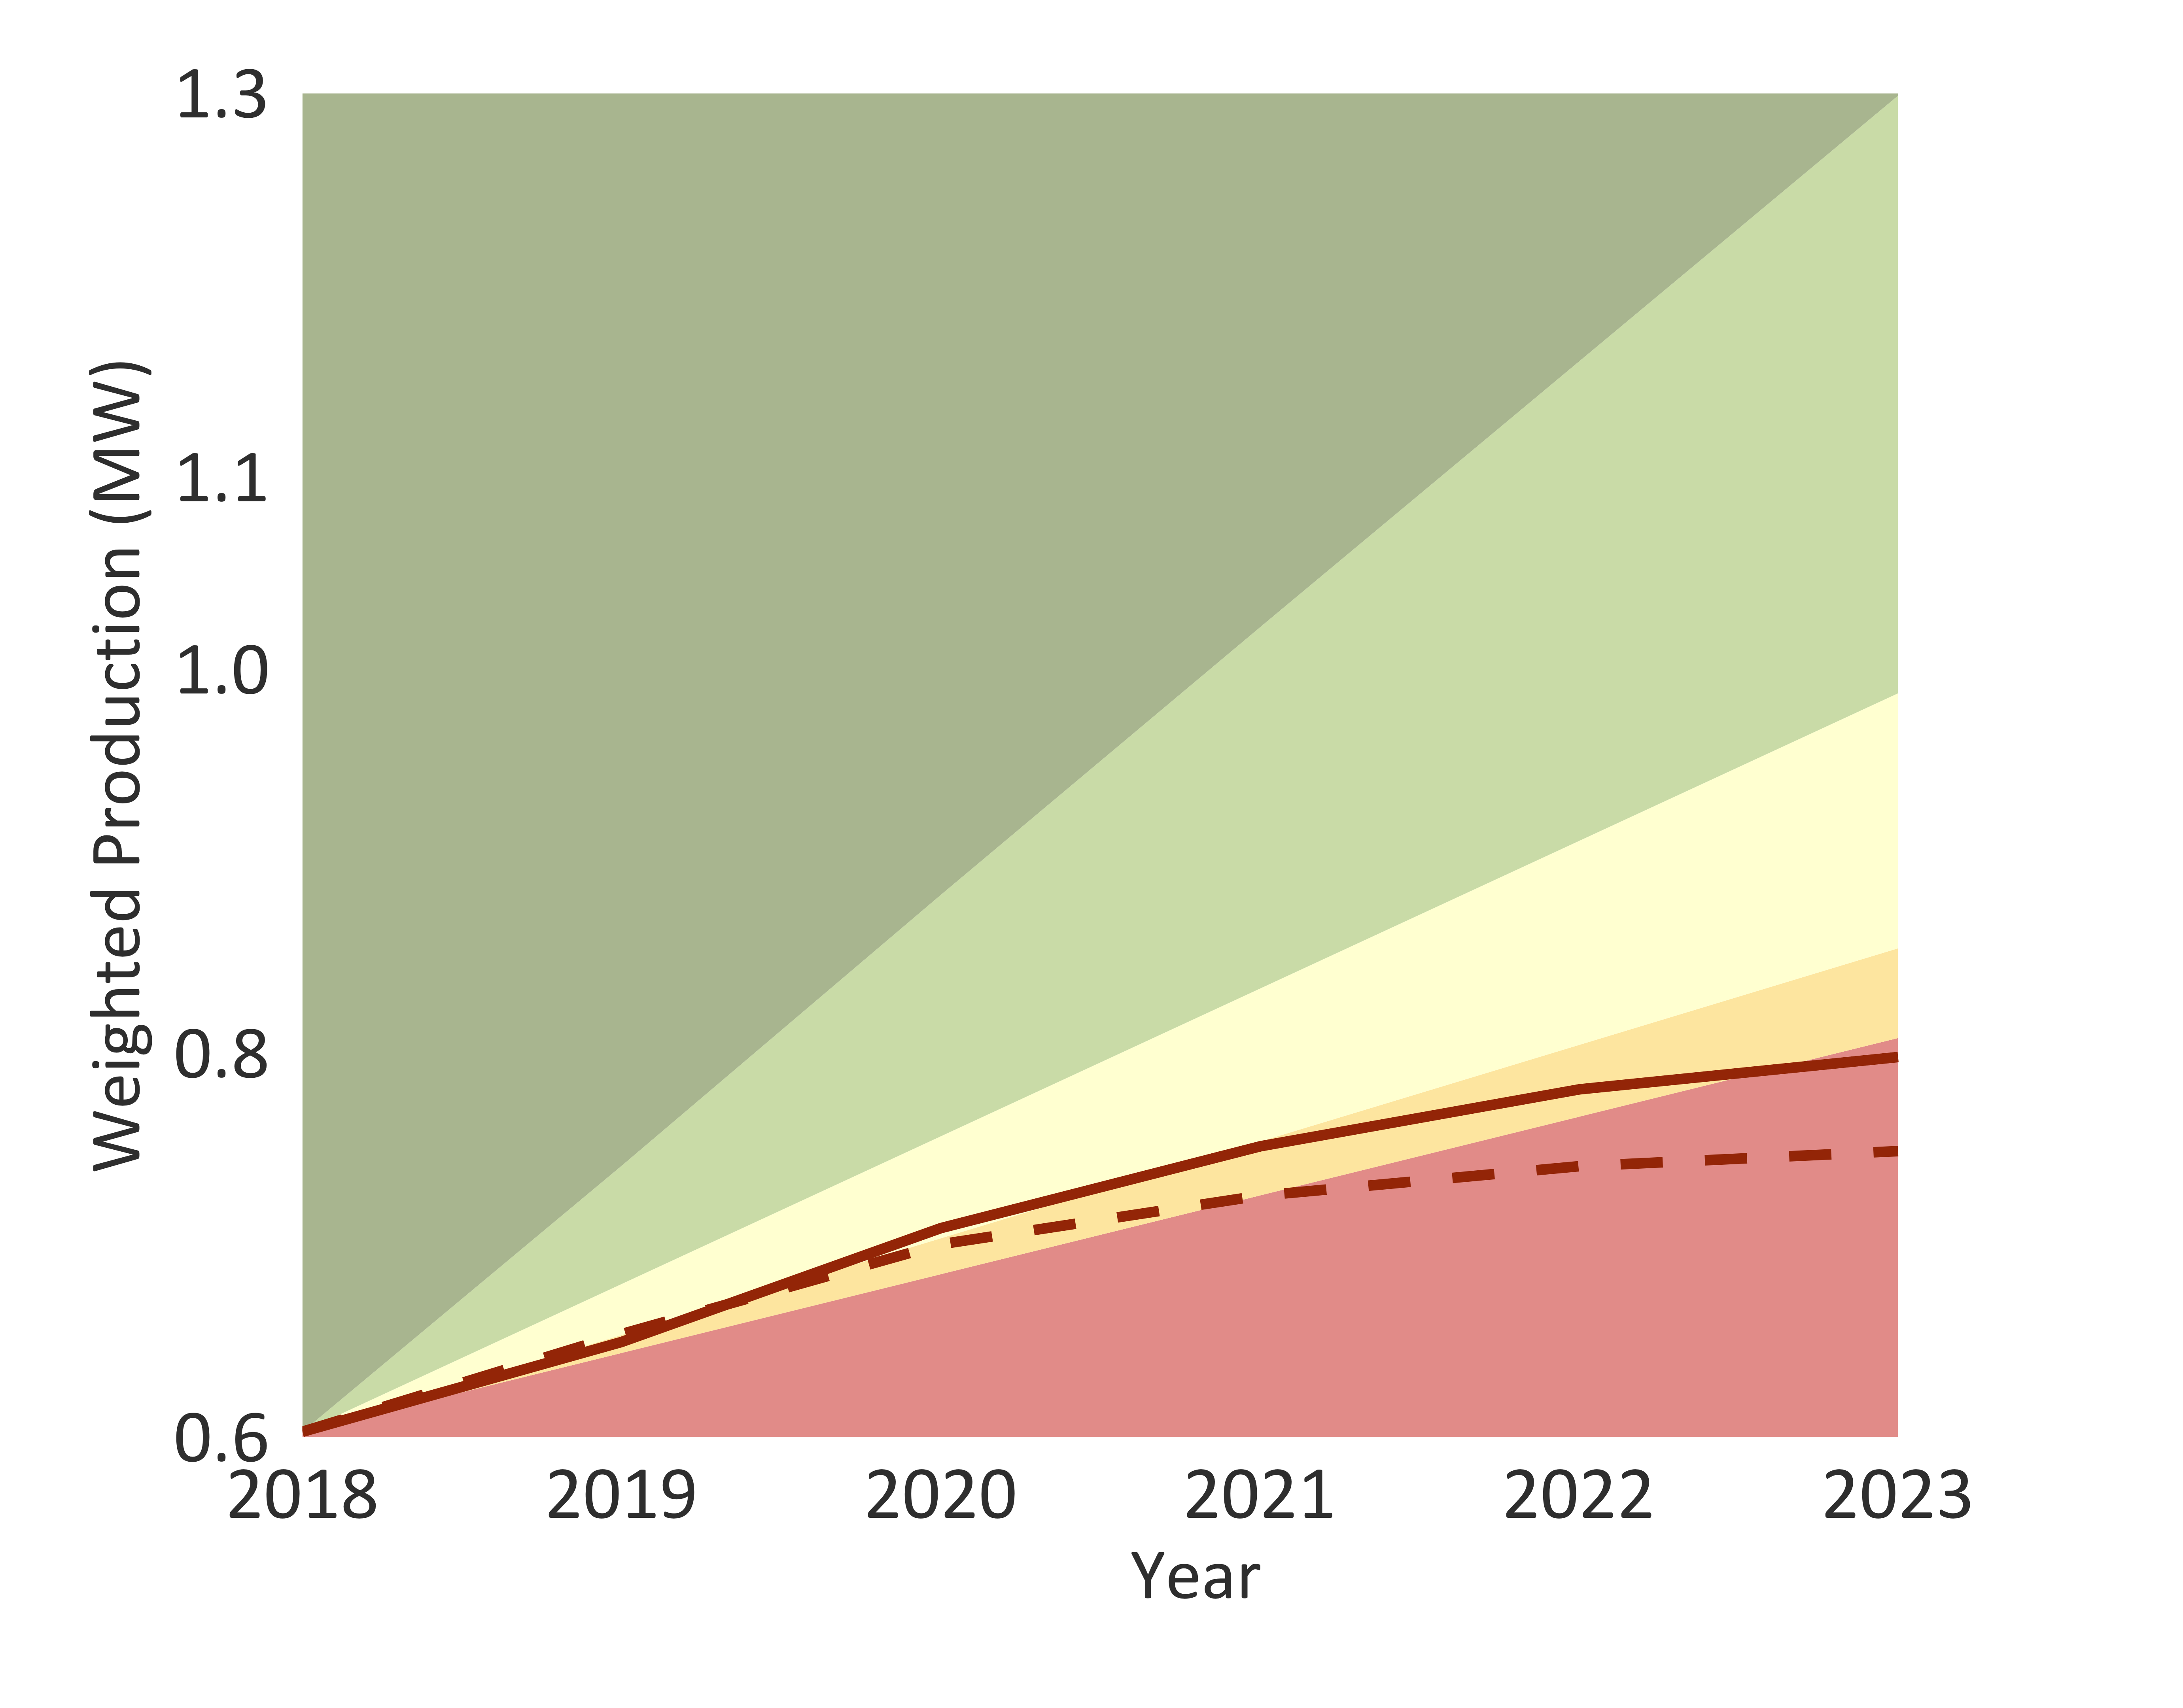
\includegraphics[trim = {0 0cm 0 0},width=1\linewidth]{CAFigures/Fig18}
		
	\end{minipage}	
	\hspace{.02\linewidth}
	\begin{minipage}[t]{.49\textwidth}
		\textbf{Trajectory of Gas Production }
		
		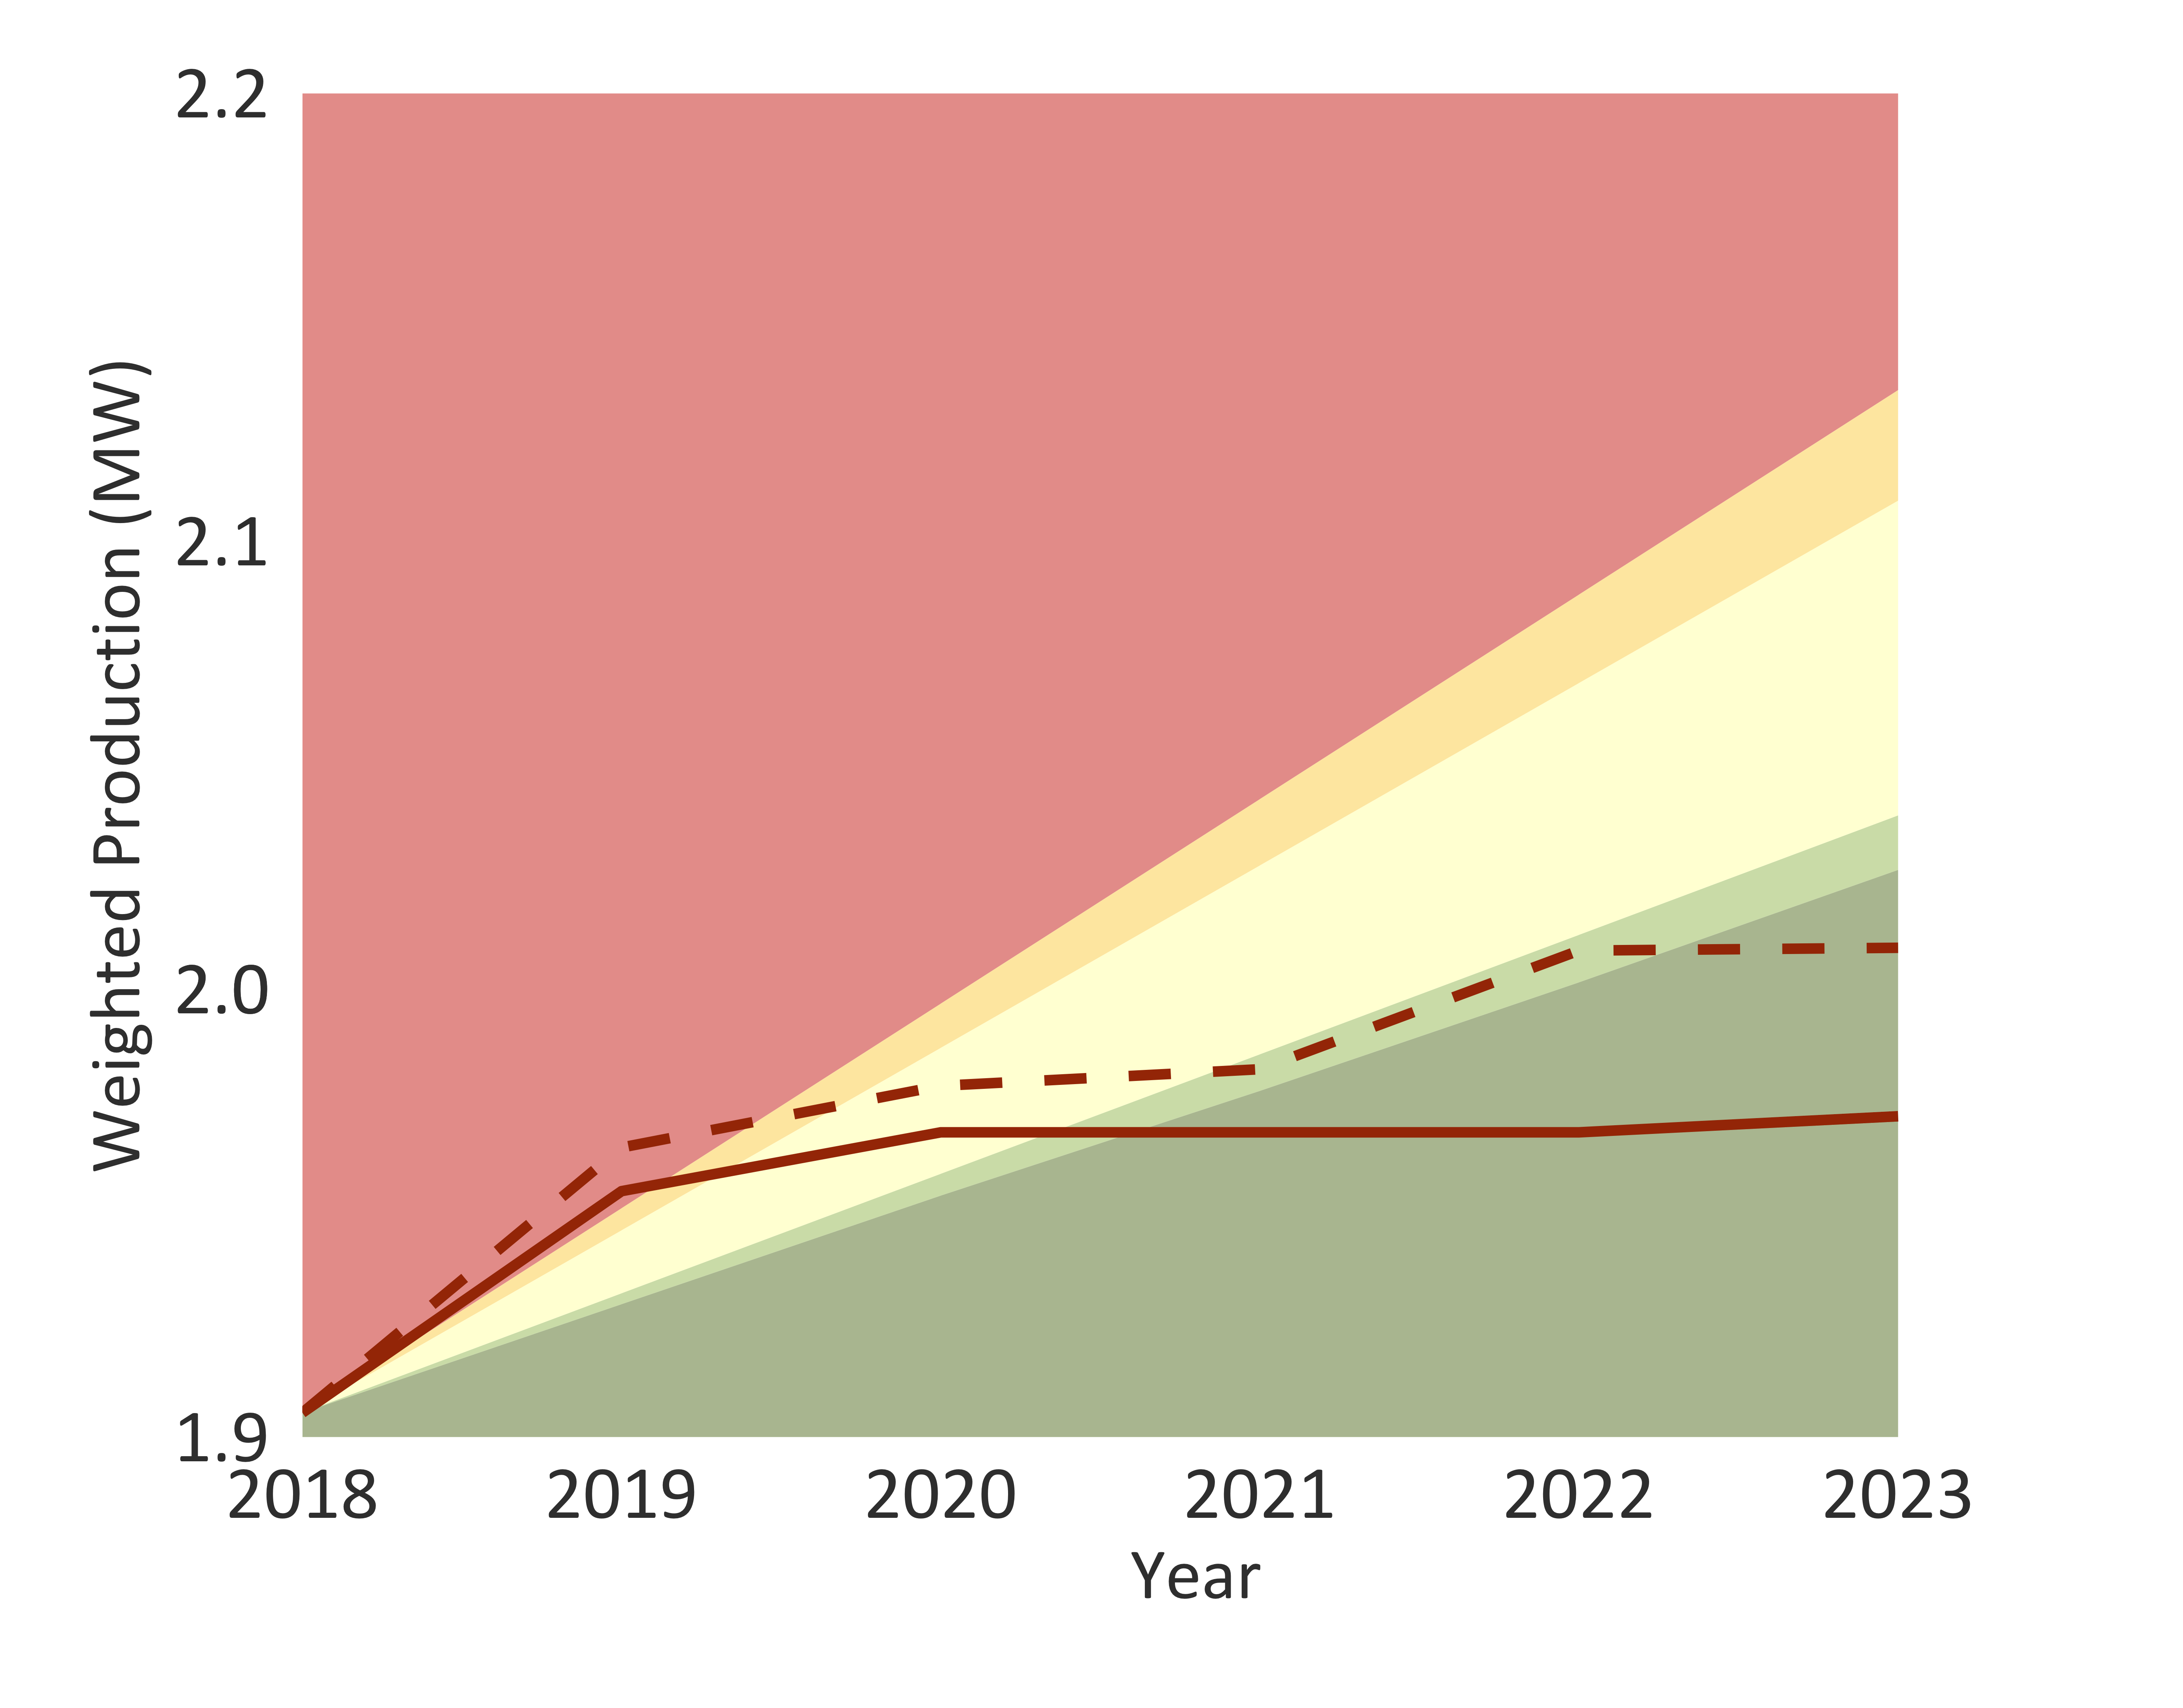
\includegraphics[trim = {0 0cm 0 0},width=1\linewidth]{CAFigures/Fig19}
		
	\end{minipage}
	
	
	\begin{center}
		\textbf{Automotive Sector}
	\end{center}
	
	\begin{minipage}[t]{.49\linewidth}
		\textbf{Trajectory of ICE Vehicle Production}
		
		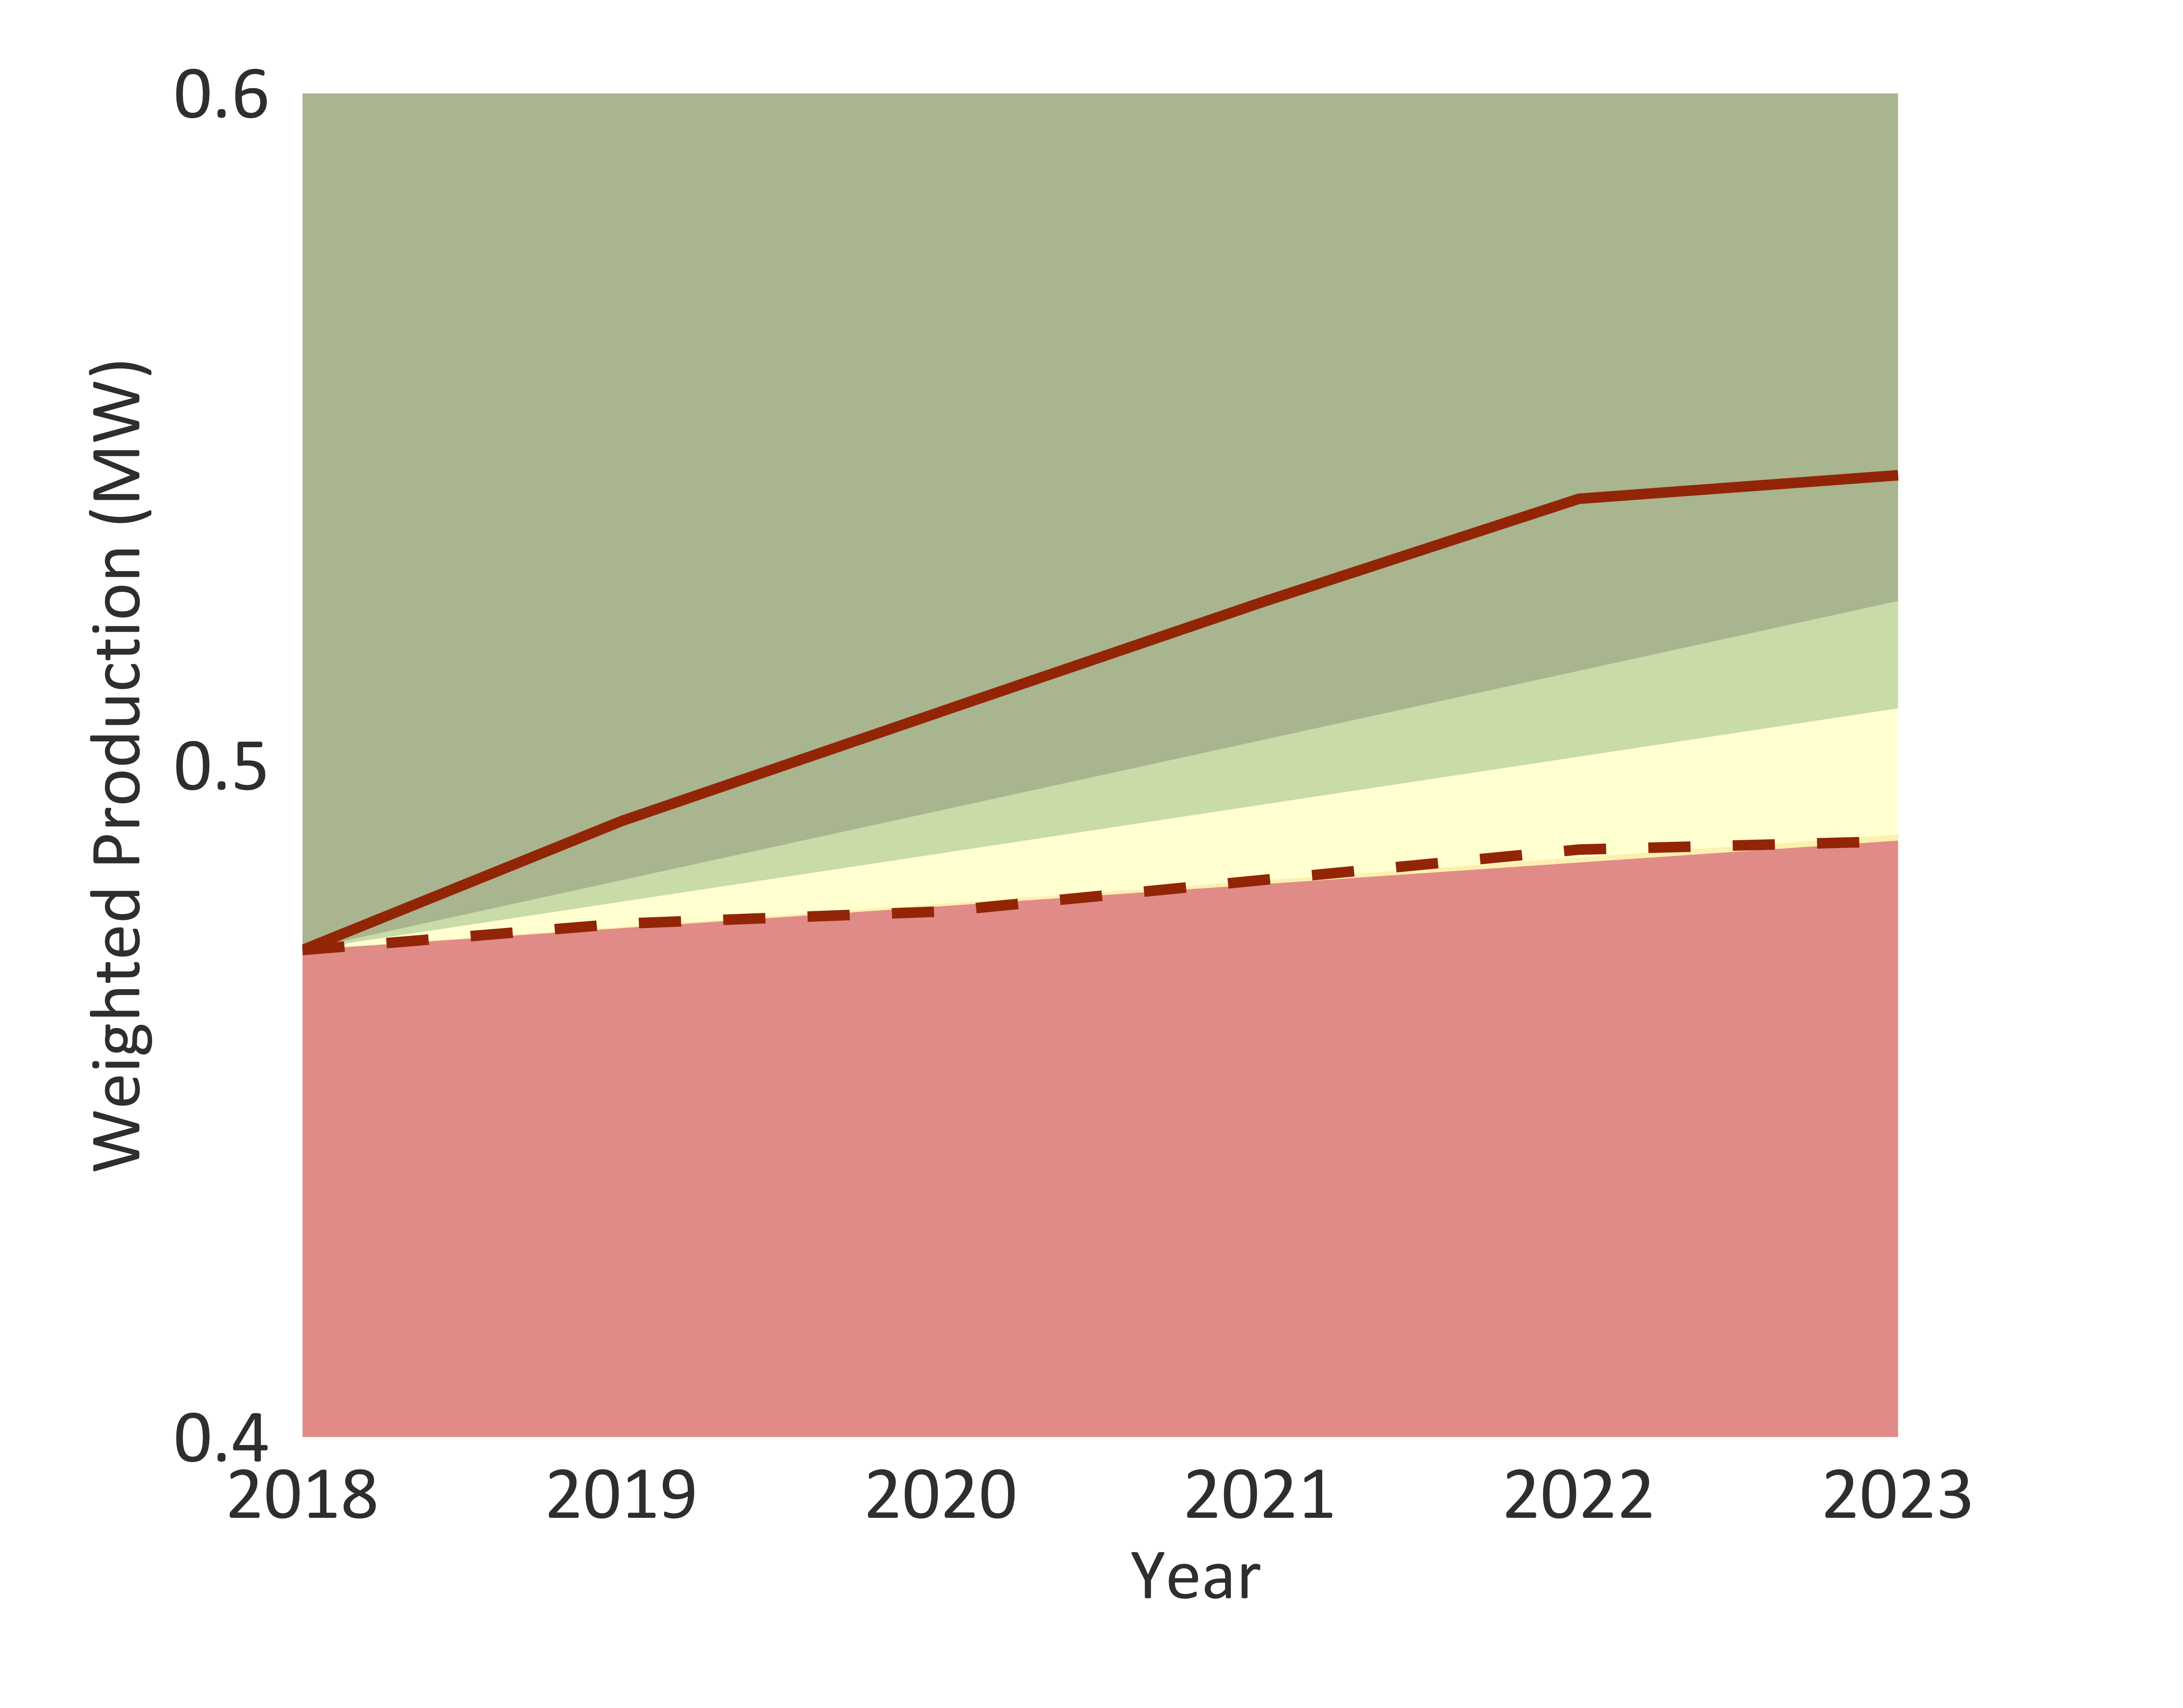
\includegraphics[trim = {0 0cm 0 0},width=1\linewidth]{CAFigures/Fig20}
		
	\end{minipage}	
	\hspace{.02\linewidth}
	\begin{minipage}[t]{.49\textwidth}
		\textbf{Trajectory of Electric Vehicle Production}
		
		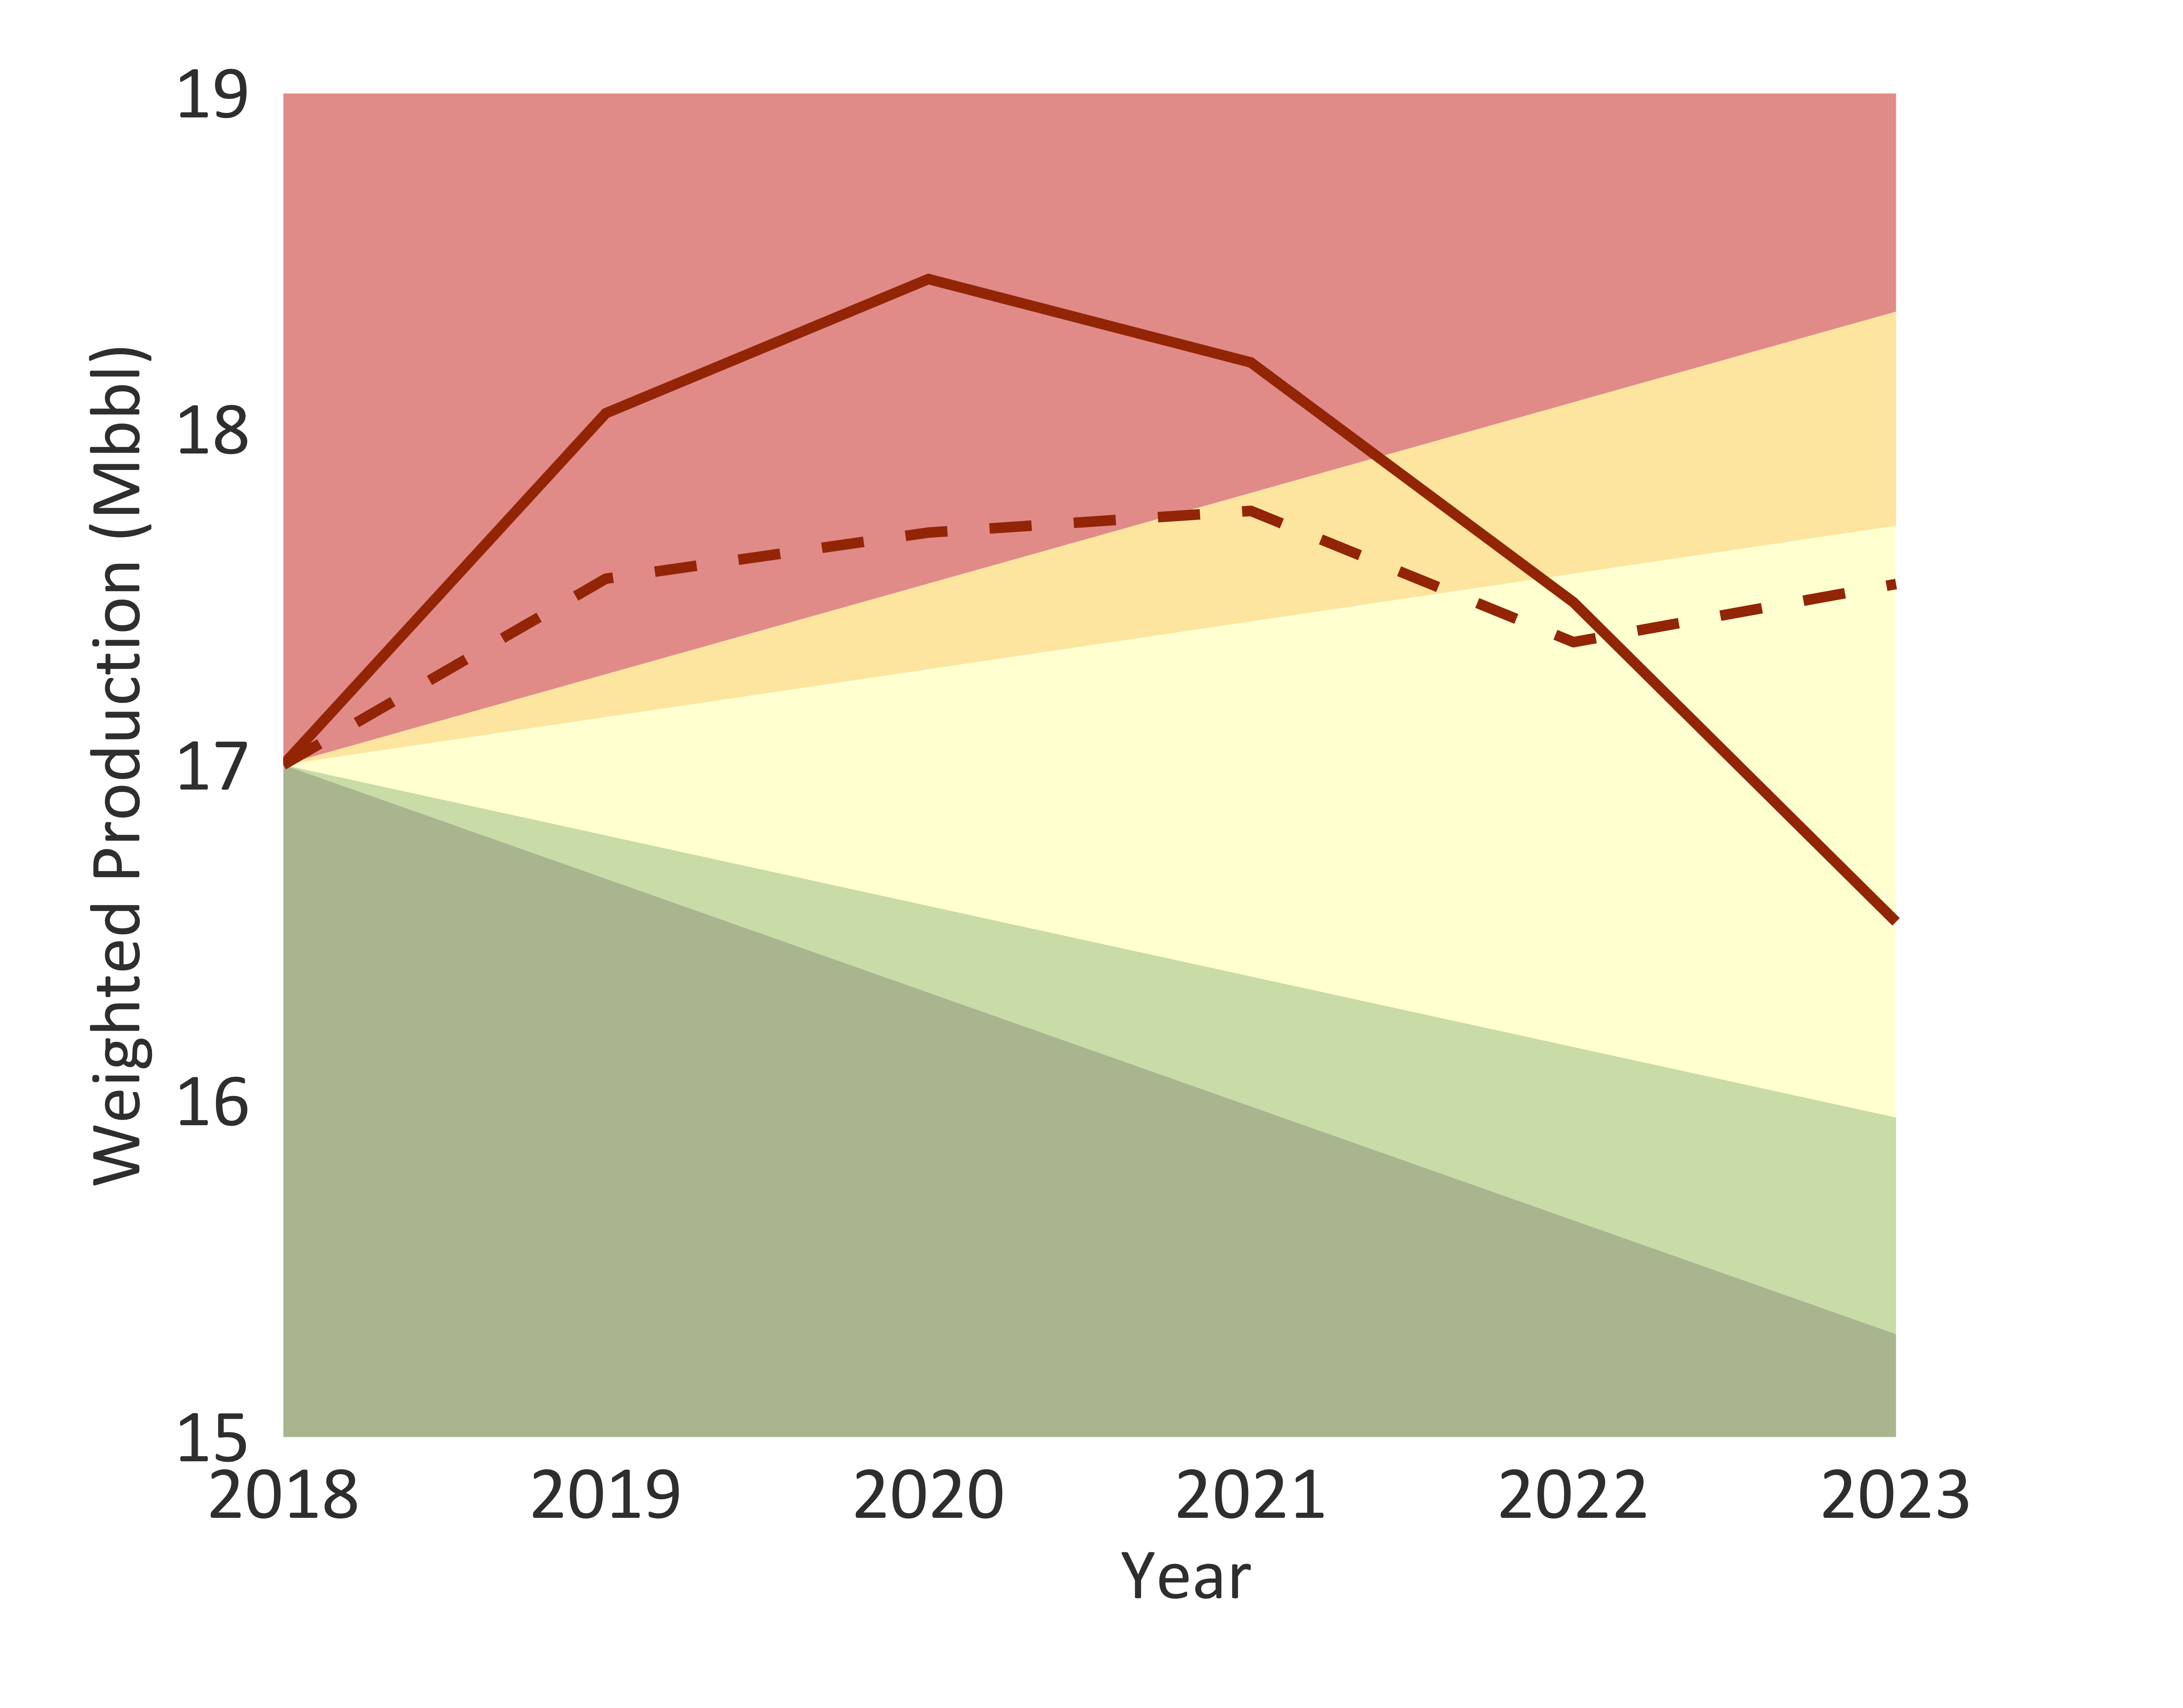
\includegraphics[trim = {0 0cm 0 0},width=1\linewidth]{CAFigures/Fig21}
		
	\end{minipage}		
	
	\vspace{-.6cm}
	\begin{center}
		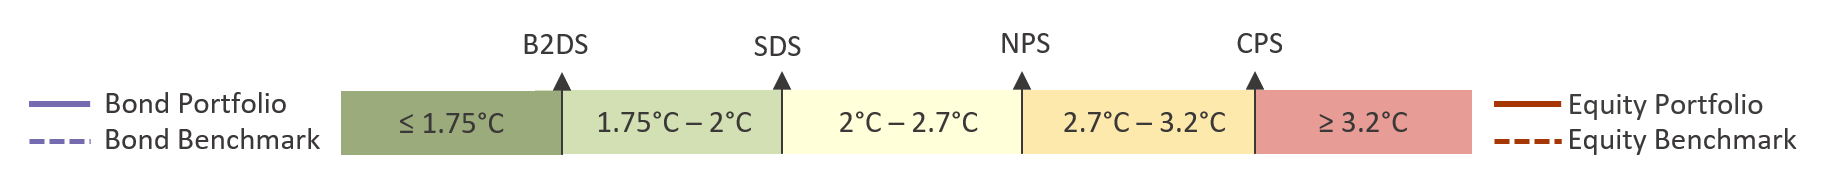
\includegraphics[trim = {0 0cm 0 0},width=.9\linewidth]{ReportGraphics/246Legend.png}
	\end{center}
	
	\PageFooterThird
	\newpage %CBSpecificE
	
	\section*{} % TRAJECTORY - EQUITY - FOSSIL FUELS AND AUTOMOTIVE %EQSpecificS p17
	\HeaderDouble{5 YEAR TREND - EQUITY}{FOSSIL FUELS AND AUTOMOTIVE}	
	
	\begin{multicols}{2}
		\textbf{The alignment graphs below show the alignment of selected fossil fuels and automobile technologies in the equity portfolio relative to the IEA scenarios for 2°C, 4°C and 6°C temperature change. } 
				For each technology, the value plotted for the portfolio (solid line) is the planned evolution or `trajectory' of fossil fuel production (top graphs) or automobile production (bottom graphs) allocated to the equity portfolio over the next 5 years.  The lines separating the color-coded background areas plot the portfolio's target production for each technology under the 2°, 4°, and 6° scenarios. The dotted line shows planned production in the specific technology for the listed equity market, scaled to the same starting point as the portfolio.                    

	\end{multicols}		
	
	\begin{center}
		\textbf{Fossil Fuel Sector}
	\end{center}
	
	\begin{minipage}[t]{.49\linewidth}
		\textbf{Trajectory of Oil Production }
		
		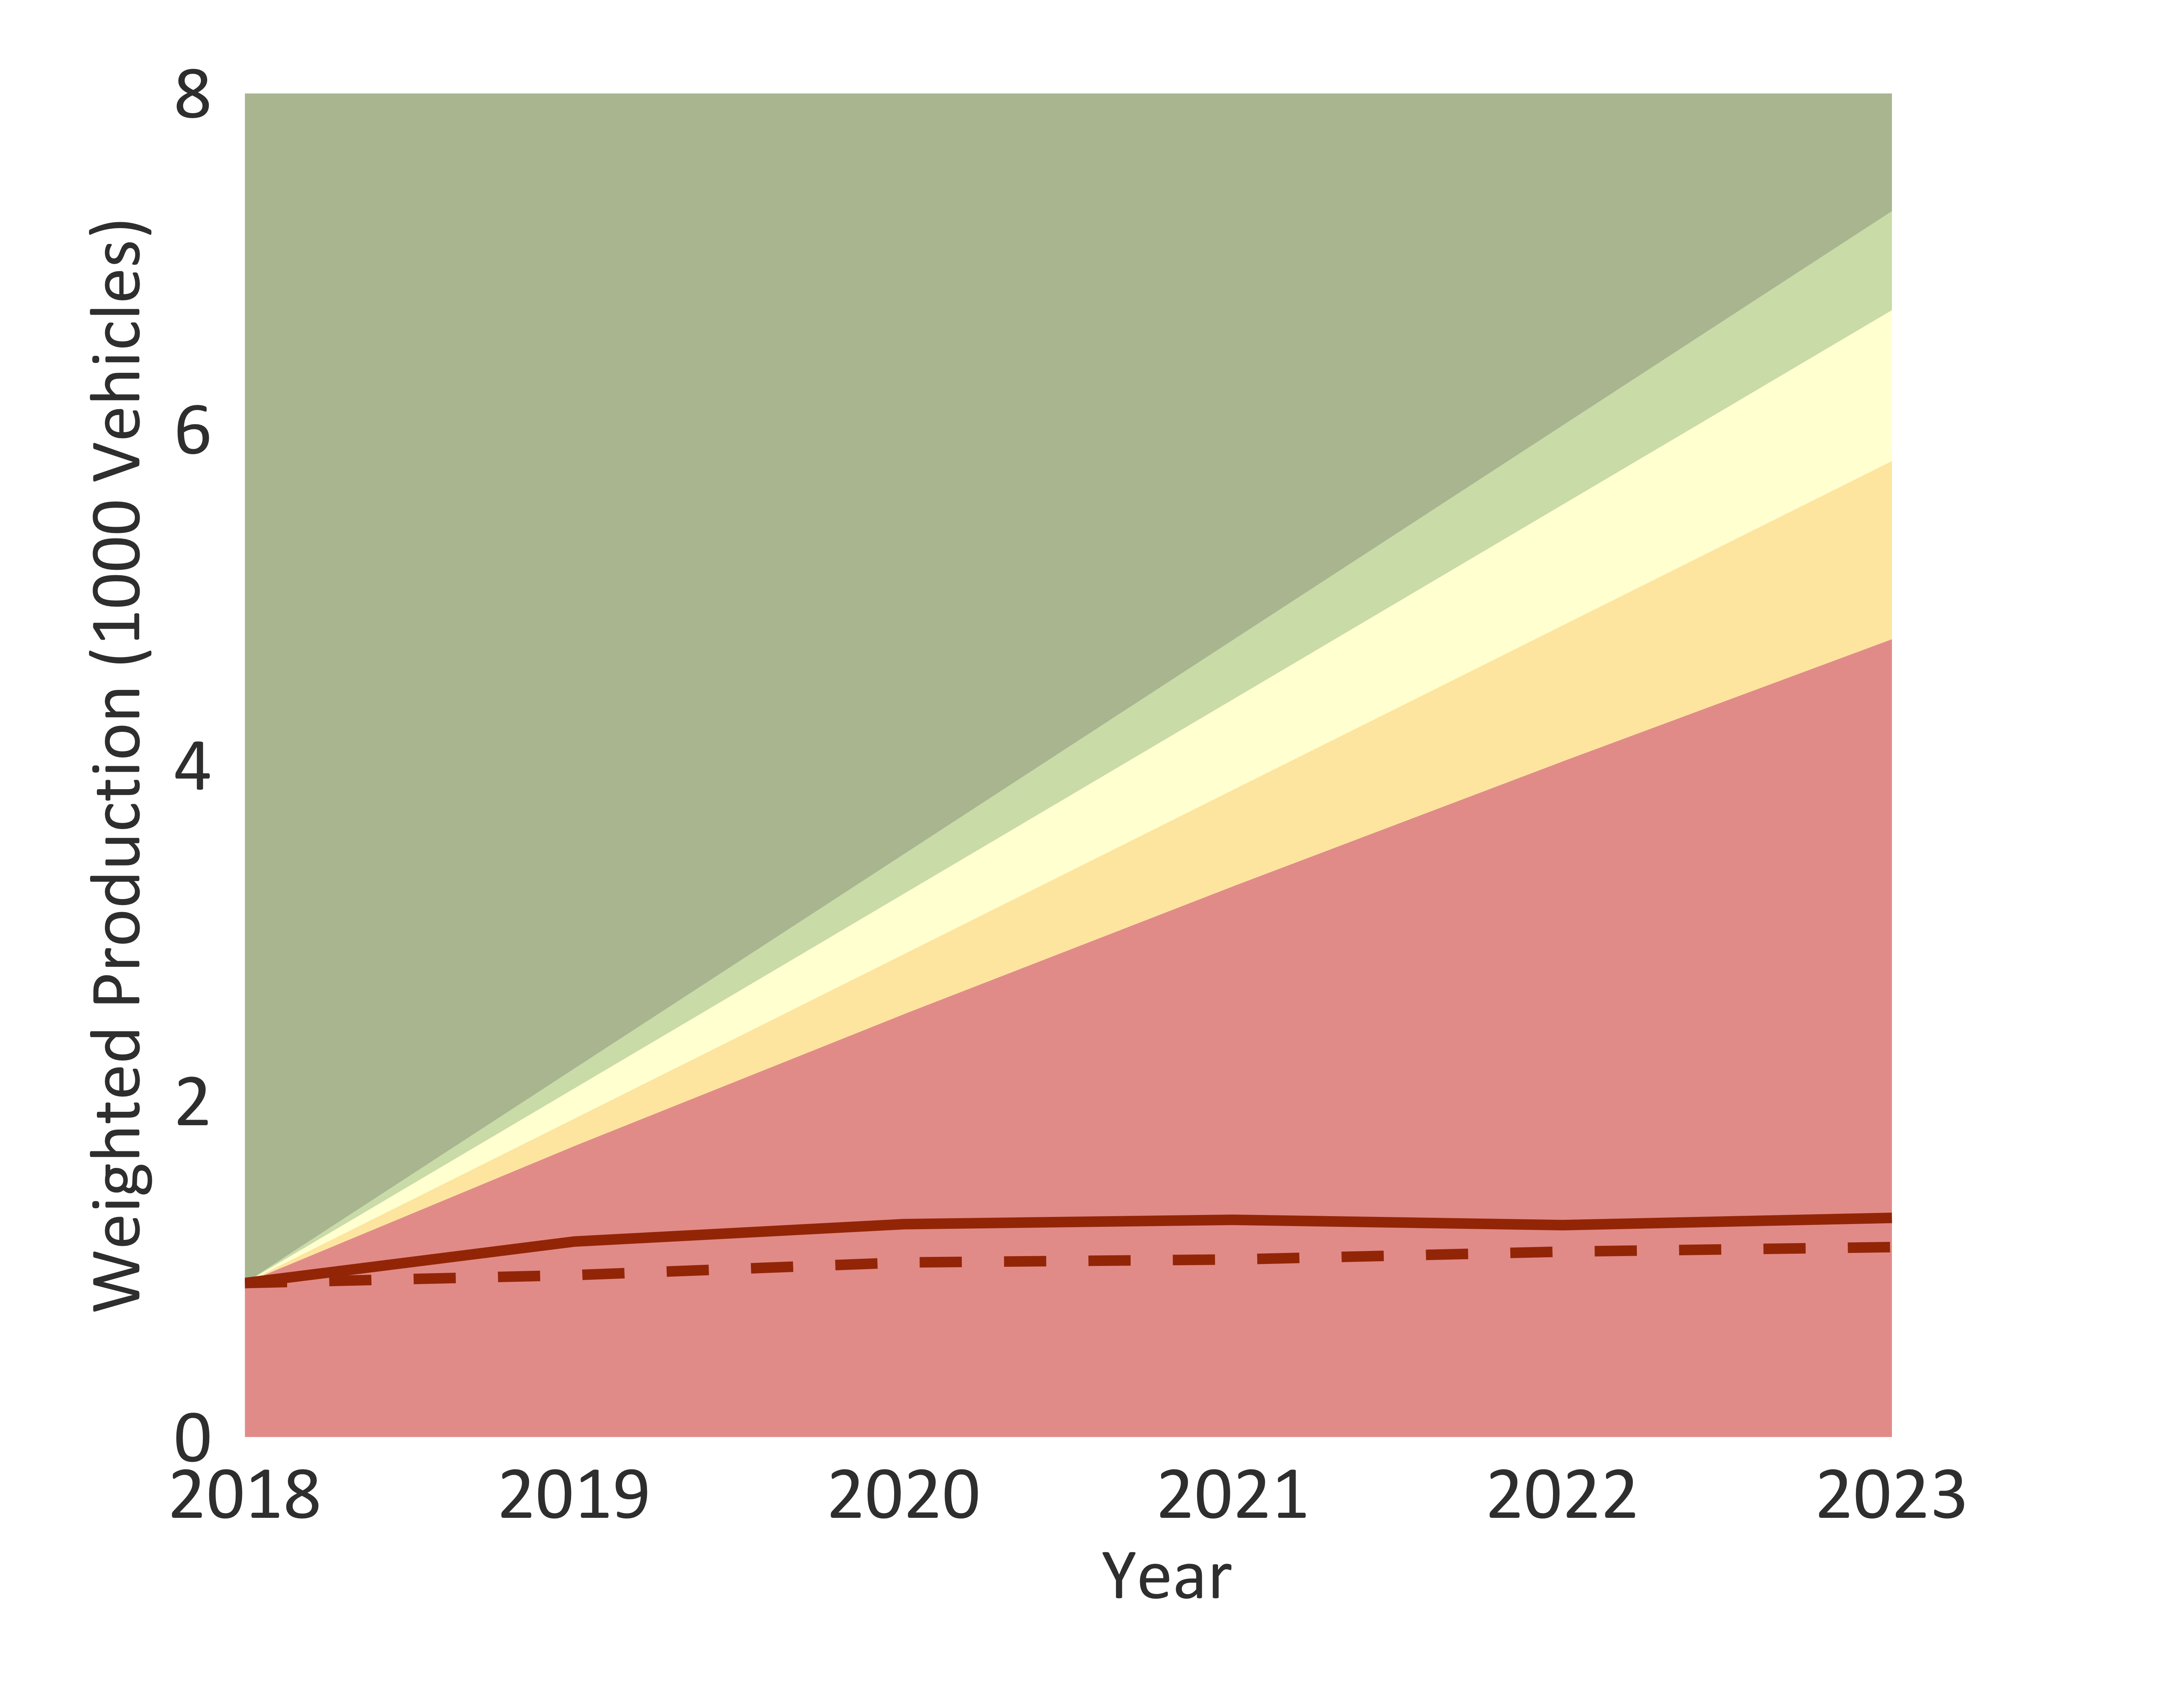
\includegraphics[trim = {0 0cm 0 0},width=1\linewidth]{CAFigures/Fig26}
		
	\end{minipage}	
	\hspace{.02\linewidth}
	\begin{minipage}[t]{.49\textwidth}
		\textbf{Trajectory of Gas Production }
		
		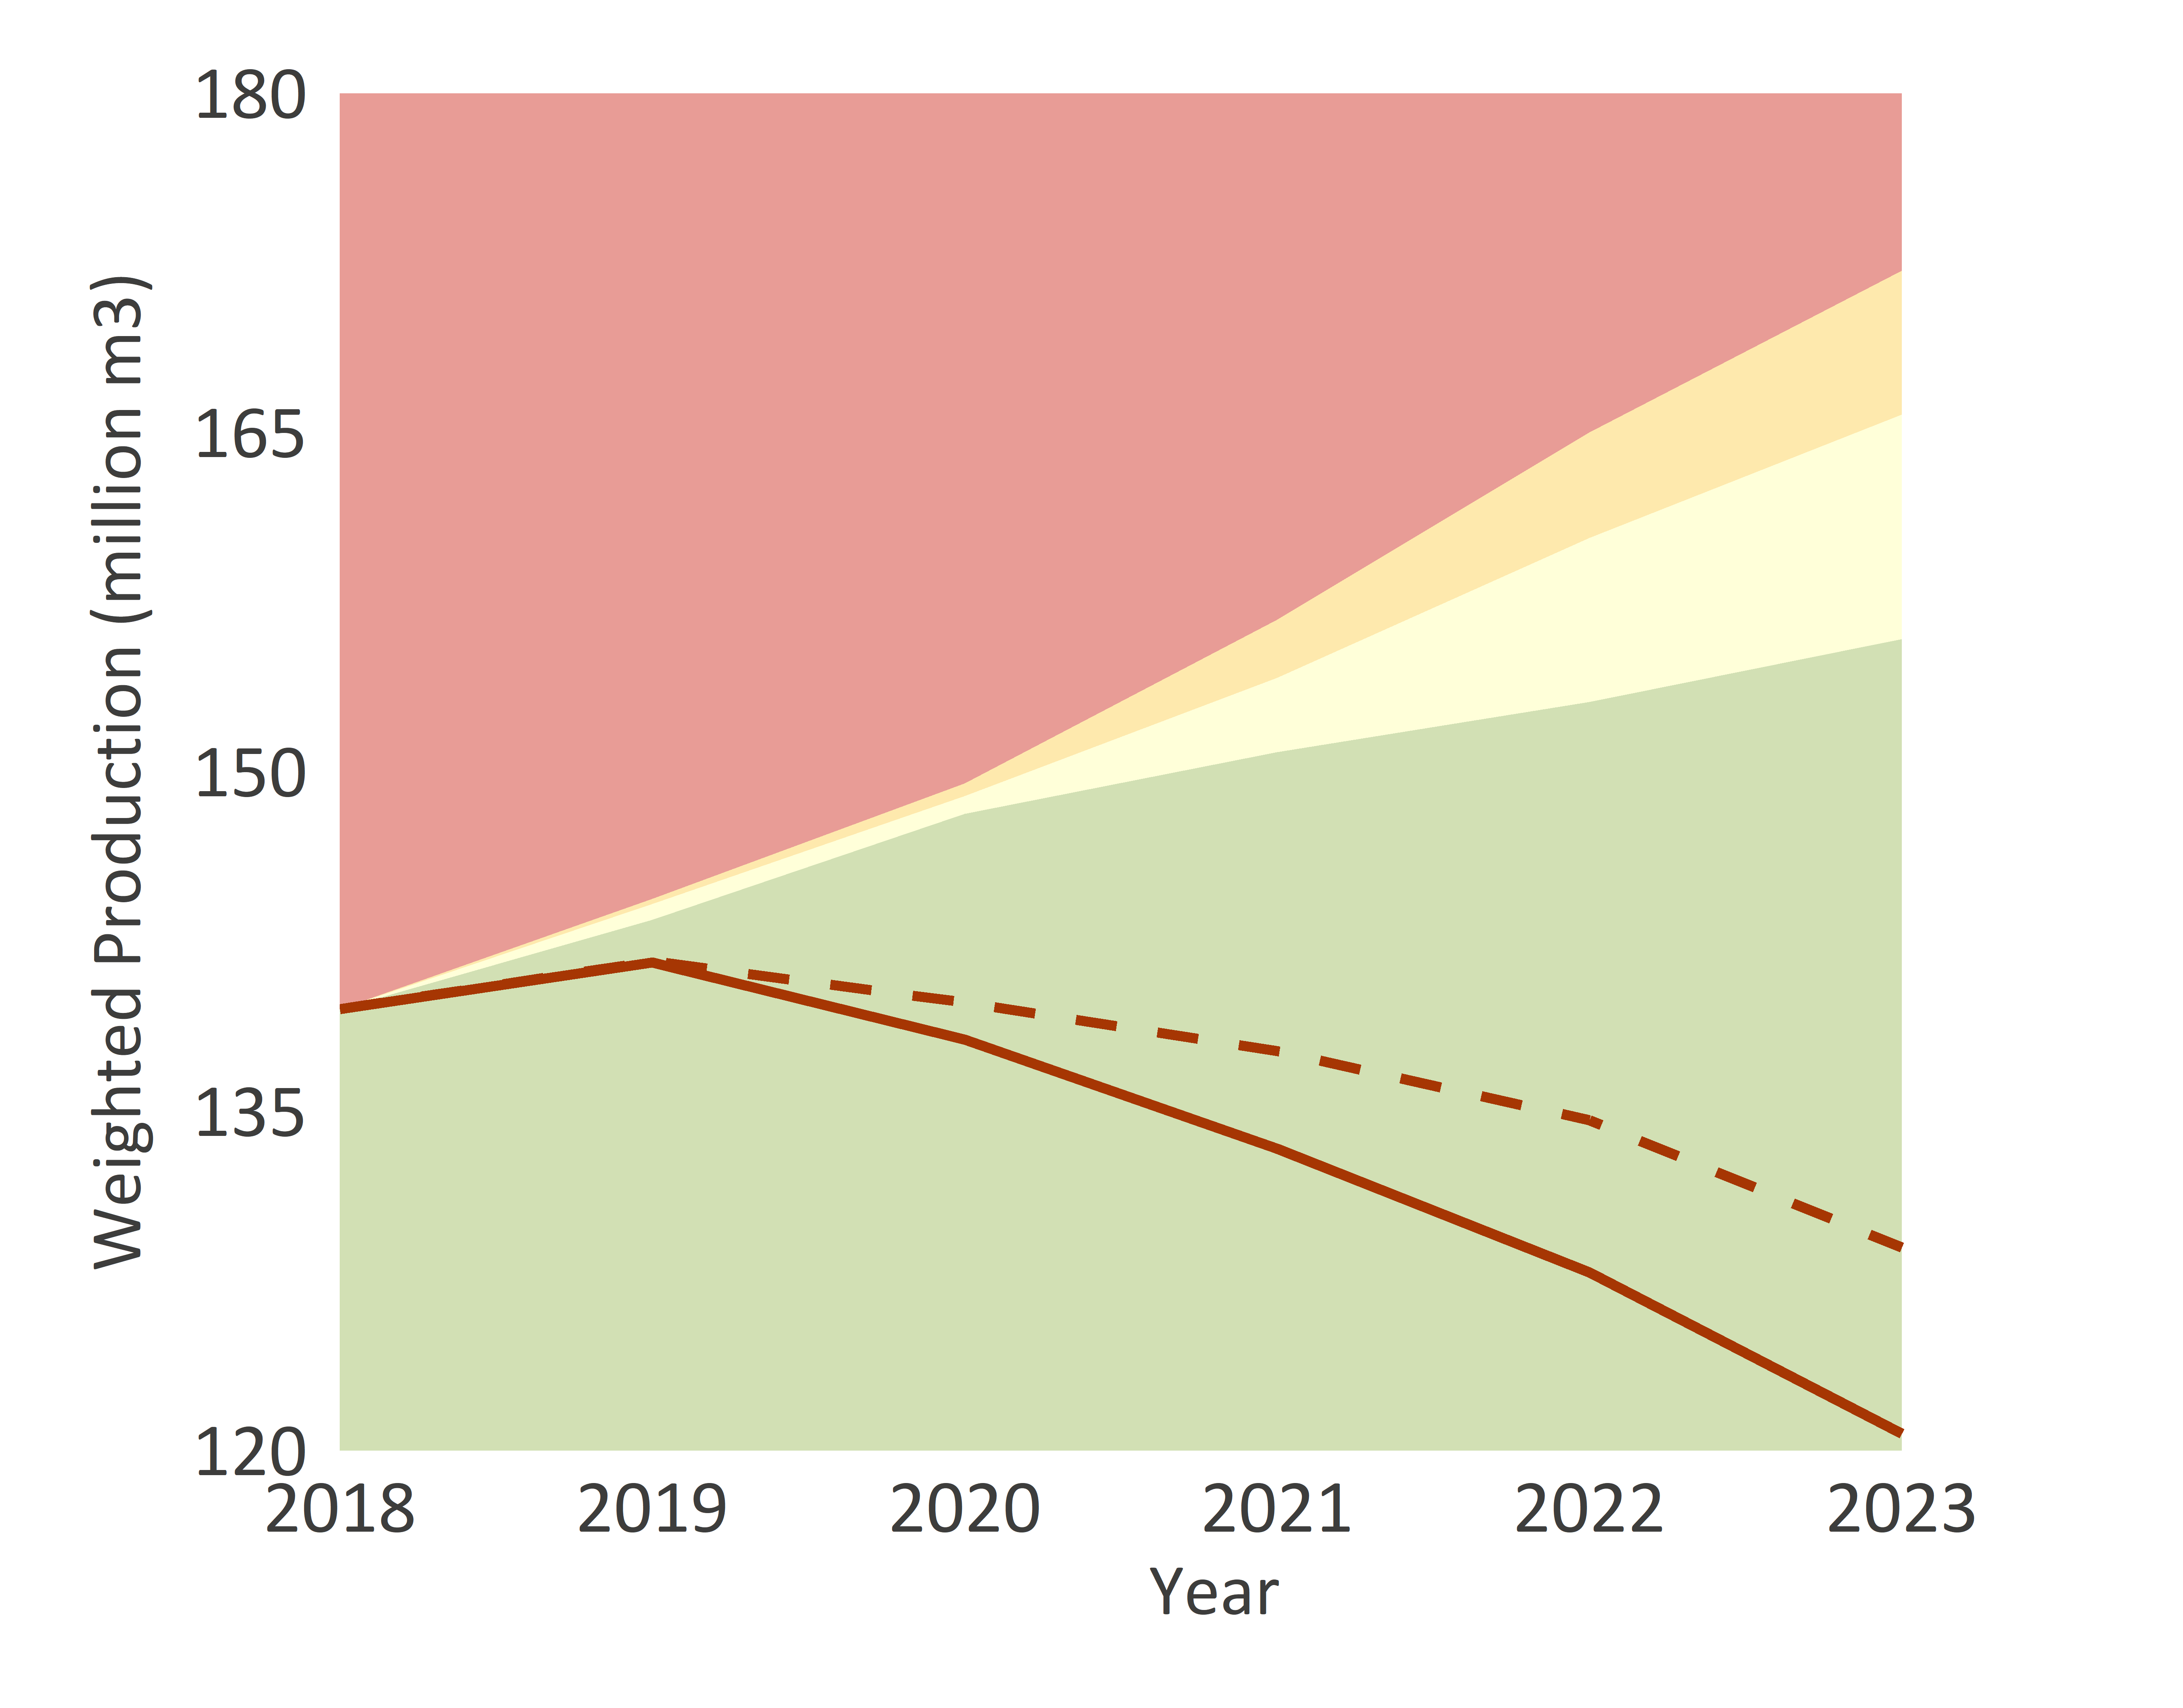
\includegraphics[trim = {0 0cm 0 0},width=1\linewidth]{CAFigures/Fig27}
		
	\end{minipage}
	
	
	\begin{center}
		\textbf{Automotive Sector}
	\end{center}
	
	\begin{minipage}[t]{.49\linewidth}
		\textbf{Trajectory of ICE Vehicle Production}
		
		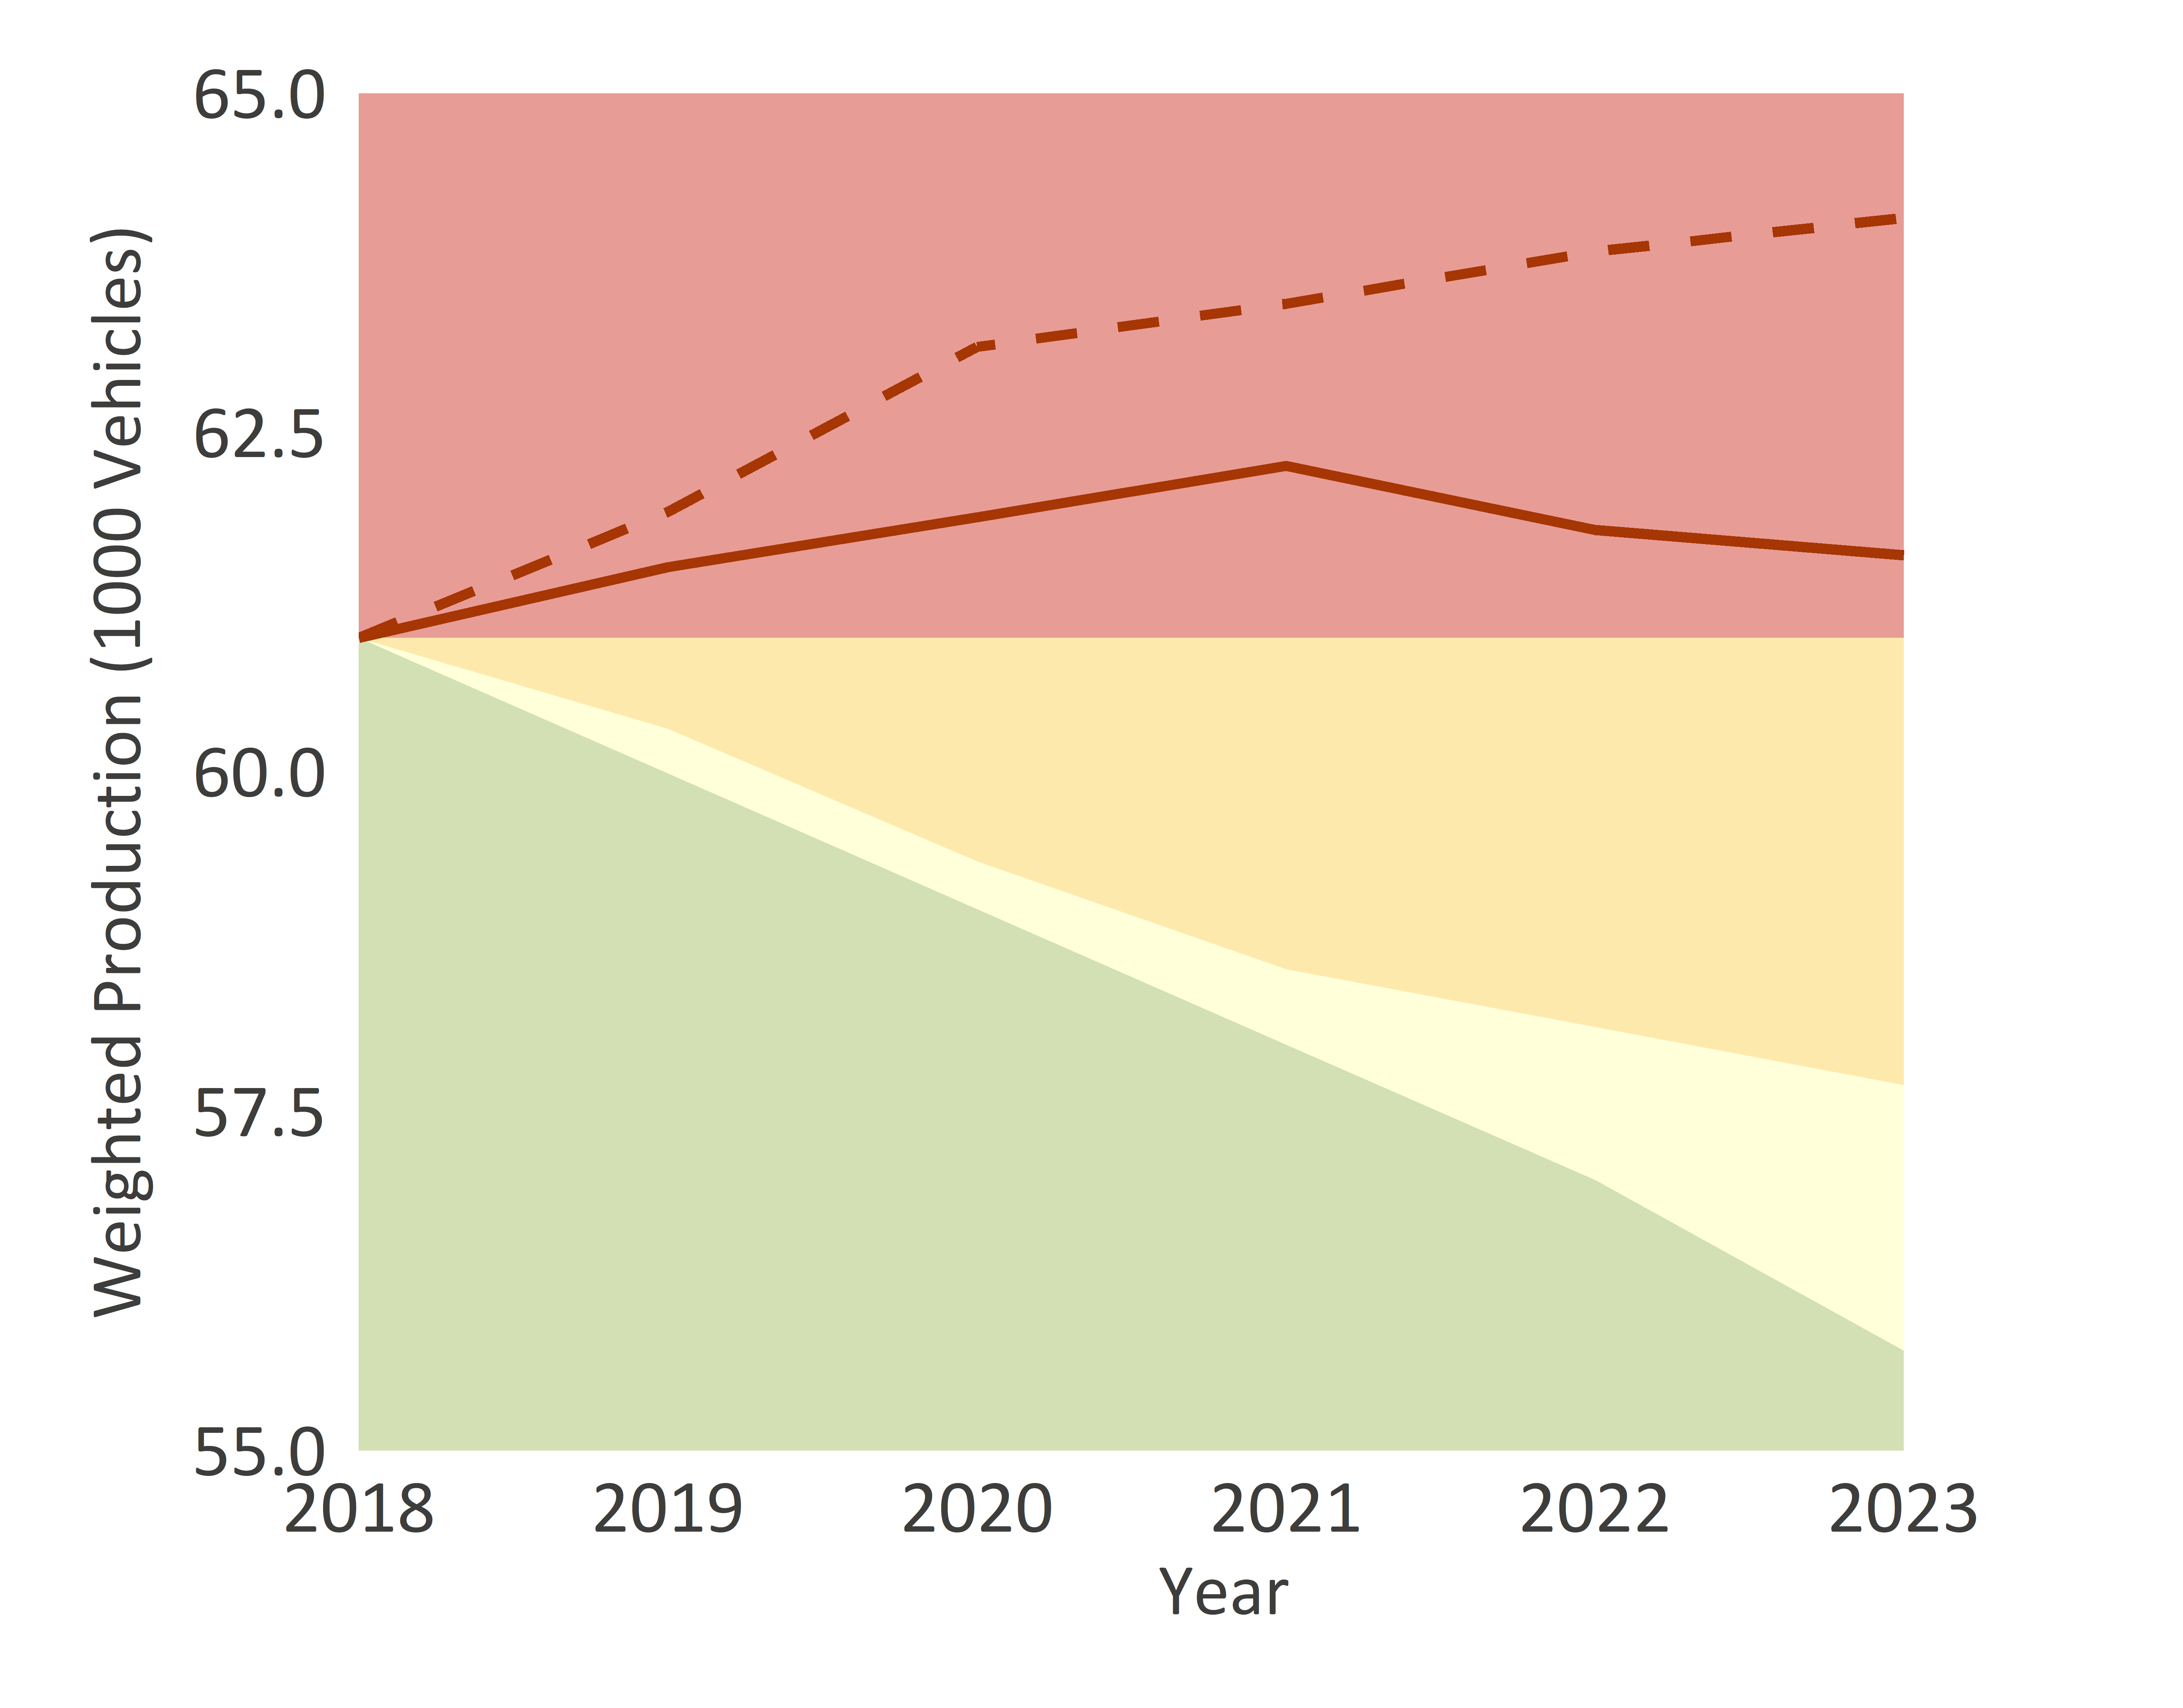
\includegraphics[trim = {0 0cm 0 0},width=1\linewidth]{CAFigures/Fig28}
		
	\end{minipage}	
	\hspace{.02\linewidth}
	\begin{minipage}[t]{.49\textwidth}
		\textbf{Trajectory of Electric Vehicle Production}
		
		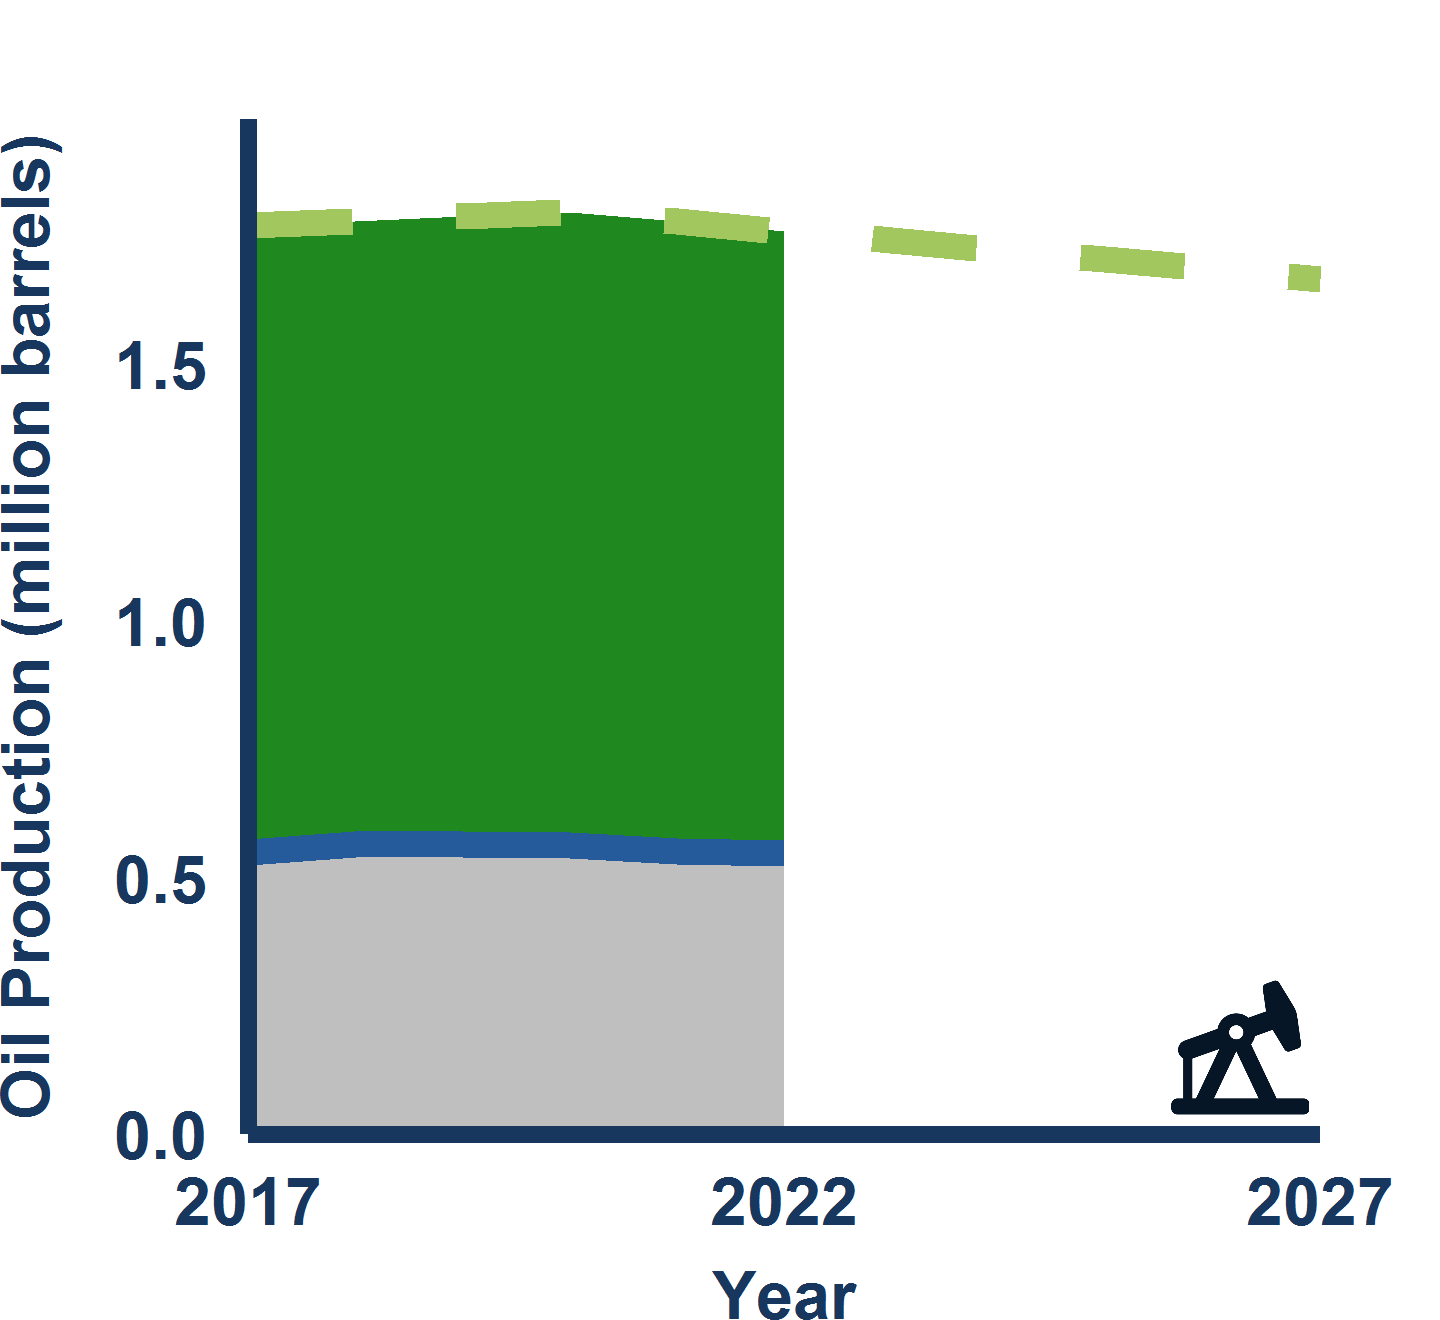
\includegraphics[trim = {0 0cm 0 0},width=1\linewidth]{CAFigures/Fig29}
		
	\end{minipage}		
	
	\vspace{-.6cm}
	\begin{center}
		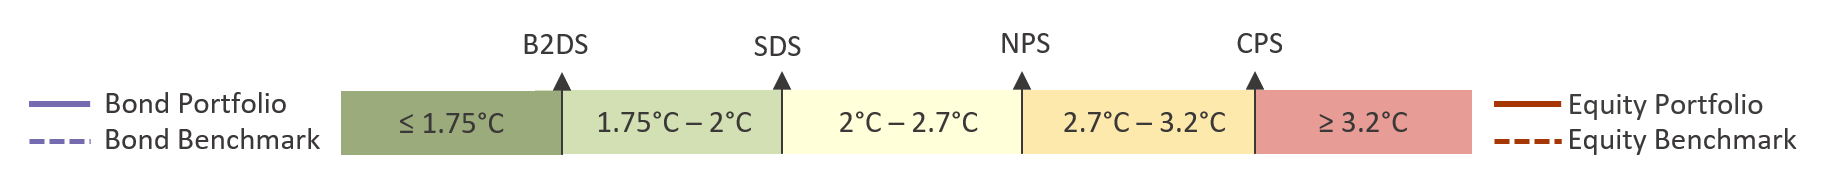
\includegraphics[trim = {0 0cm 0 0},width=.9\linewidth]{ReportGraphics/246Legend.png}
	\end{center}
	
	\PageFooterThird
	\newpage %EQSpecificE
	\section*{} % 4th SECTION 
	\SectionHeadingDouble{SECTION 4:}{THE EXPOSURE OF THE PORTFOLIO}{TO 2°C SCENARIOS IN 2023}
	
	
	\newpage
	\section*{} % FUTURE TECHNOLOGY SHARE p19
	\HeaderSingle{FUTURE TECHNOLOGY SHARE}
	
	\begin{multicols}{2}
		\textbf{The figure below shows the estimated exposure in 2023 to high-carbon and low-carbon technologies for the fossil fuel, power, and automotive sectors, in both the fixed income and equity portfolios. }
		
		The results are a function both of the starting point of the exposure (Section 2) and the evolution of the exposure over time (Section 3) based on current revealed investment and production plans for all technologies.  The `Portfolio' column shows the relative share of each technology within each sector for this portfolio.  This can then be compared to the relative technology share of both the aggregated portfolio of all California insurers included in the analysis (`All Insurers') as well as the expected market technology mix under a 2°C transition in 2023 (`2° Market Benchmark').
		
		As highlighted previously, the analysis does not include assumptions around changes in portfolio composition. Rather, it is limited to how the portfolio's  exposure to high-carbon and low-carbon technologies is set to change over time as a function of changes in company exposures, independent of portfolio composition changes. The results help contextualize the share of the sectoral exposure in 2023 exposed to transition risks in terms of the share of activities that can be classified as either high-carbon or low-carbon. Given the marginal nature of renewable activities across oil and gas companies, this share has not been considered in the analysis, although it may over time represent a growing share. 
		
	\end{multicols}
	
	
	\textbf{Fixed Income}
	
	
	\begin{center}
		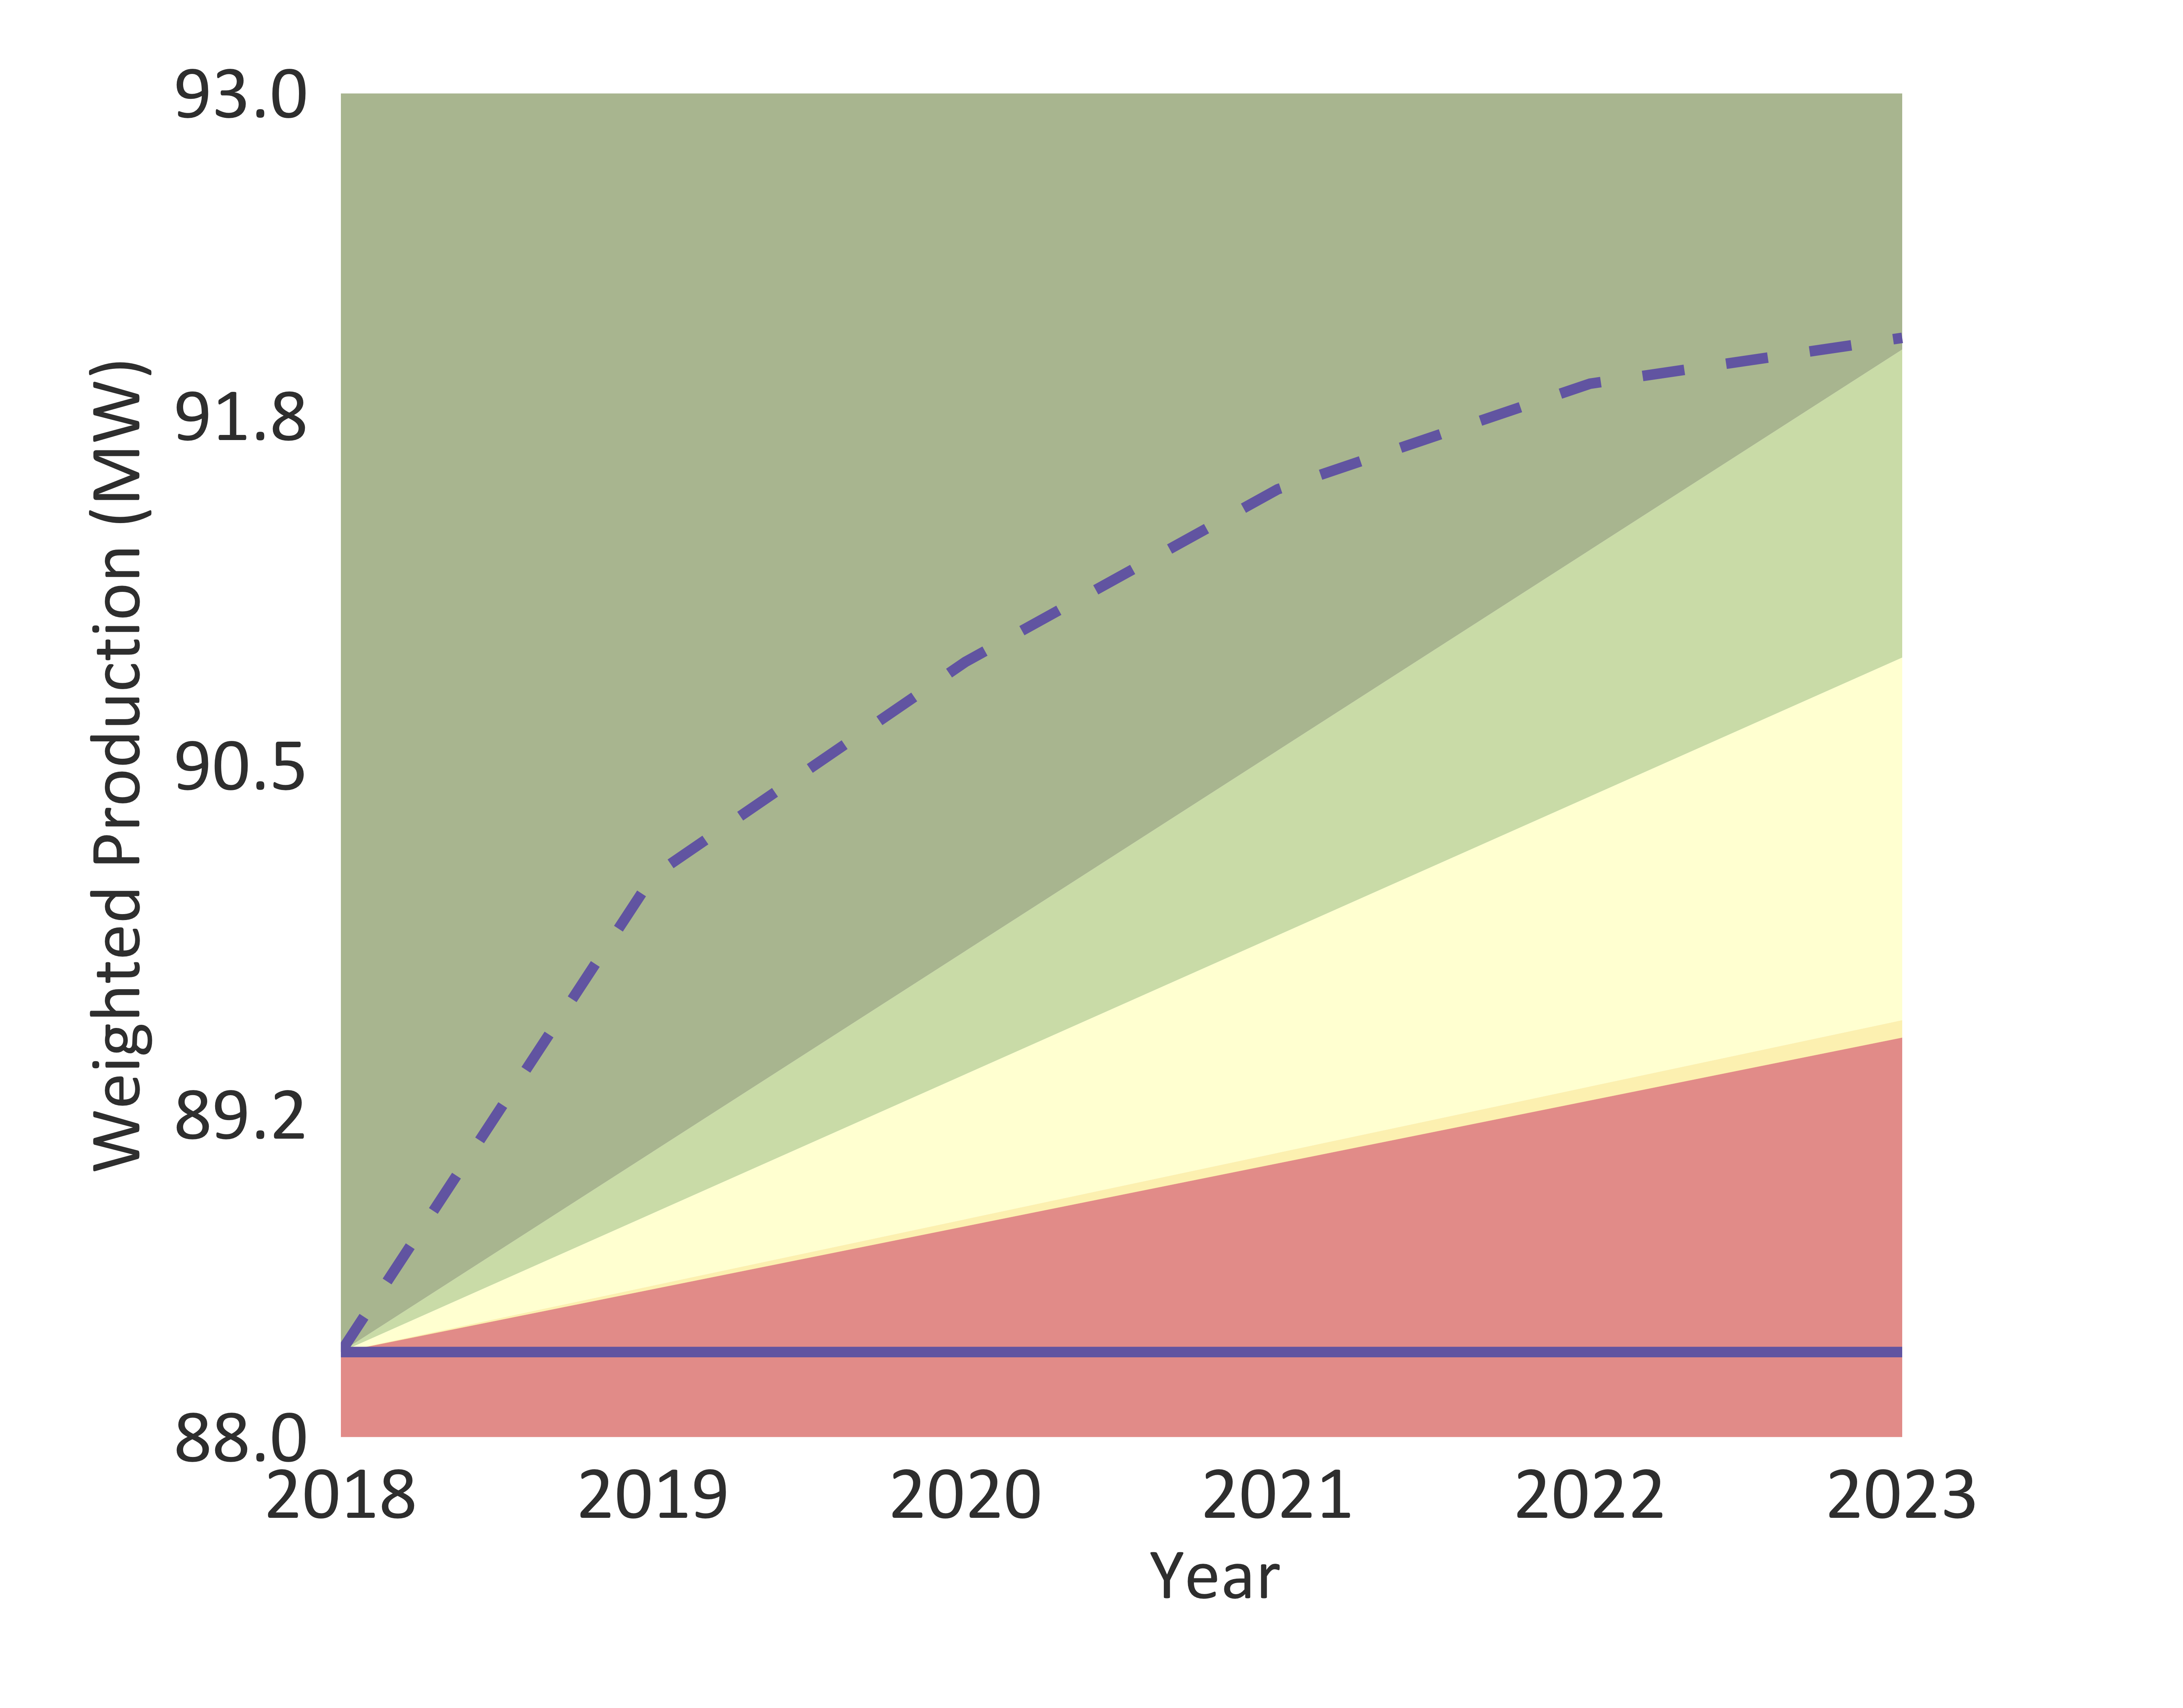
\includegraphics[trim = {0 0cm 0 0},width=1\linewidth]{CAFigures/Fig10}
	\end{center}
	
	

	\textbf{Equity}
	
	
	\begin{center}
		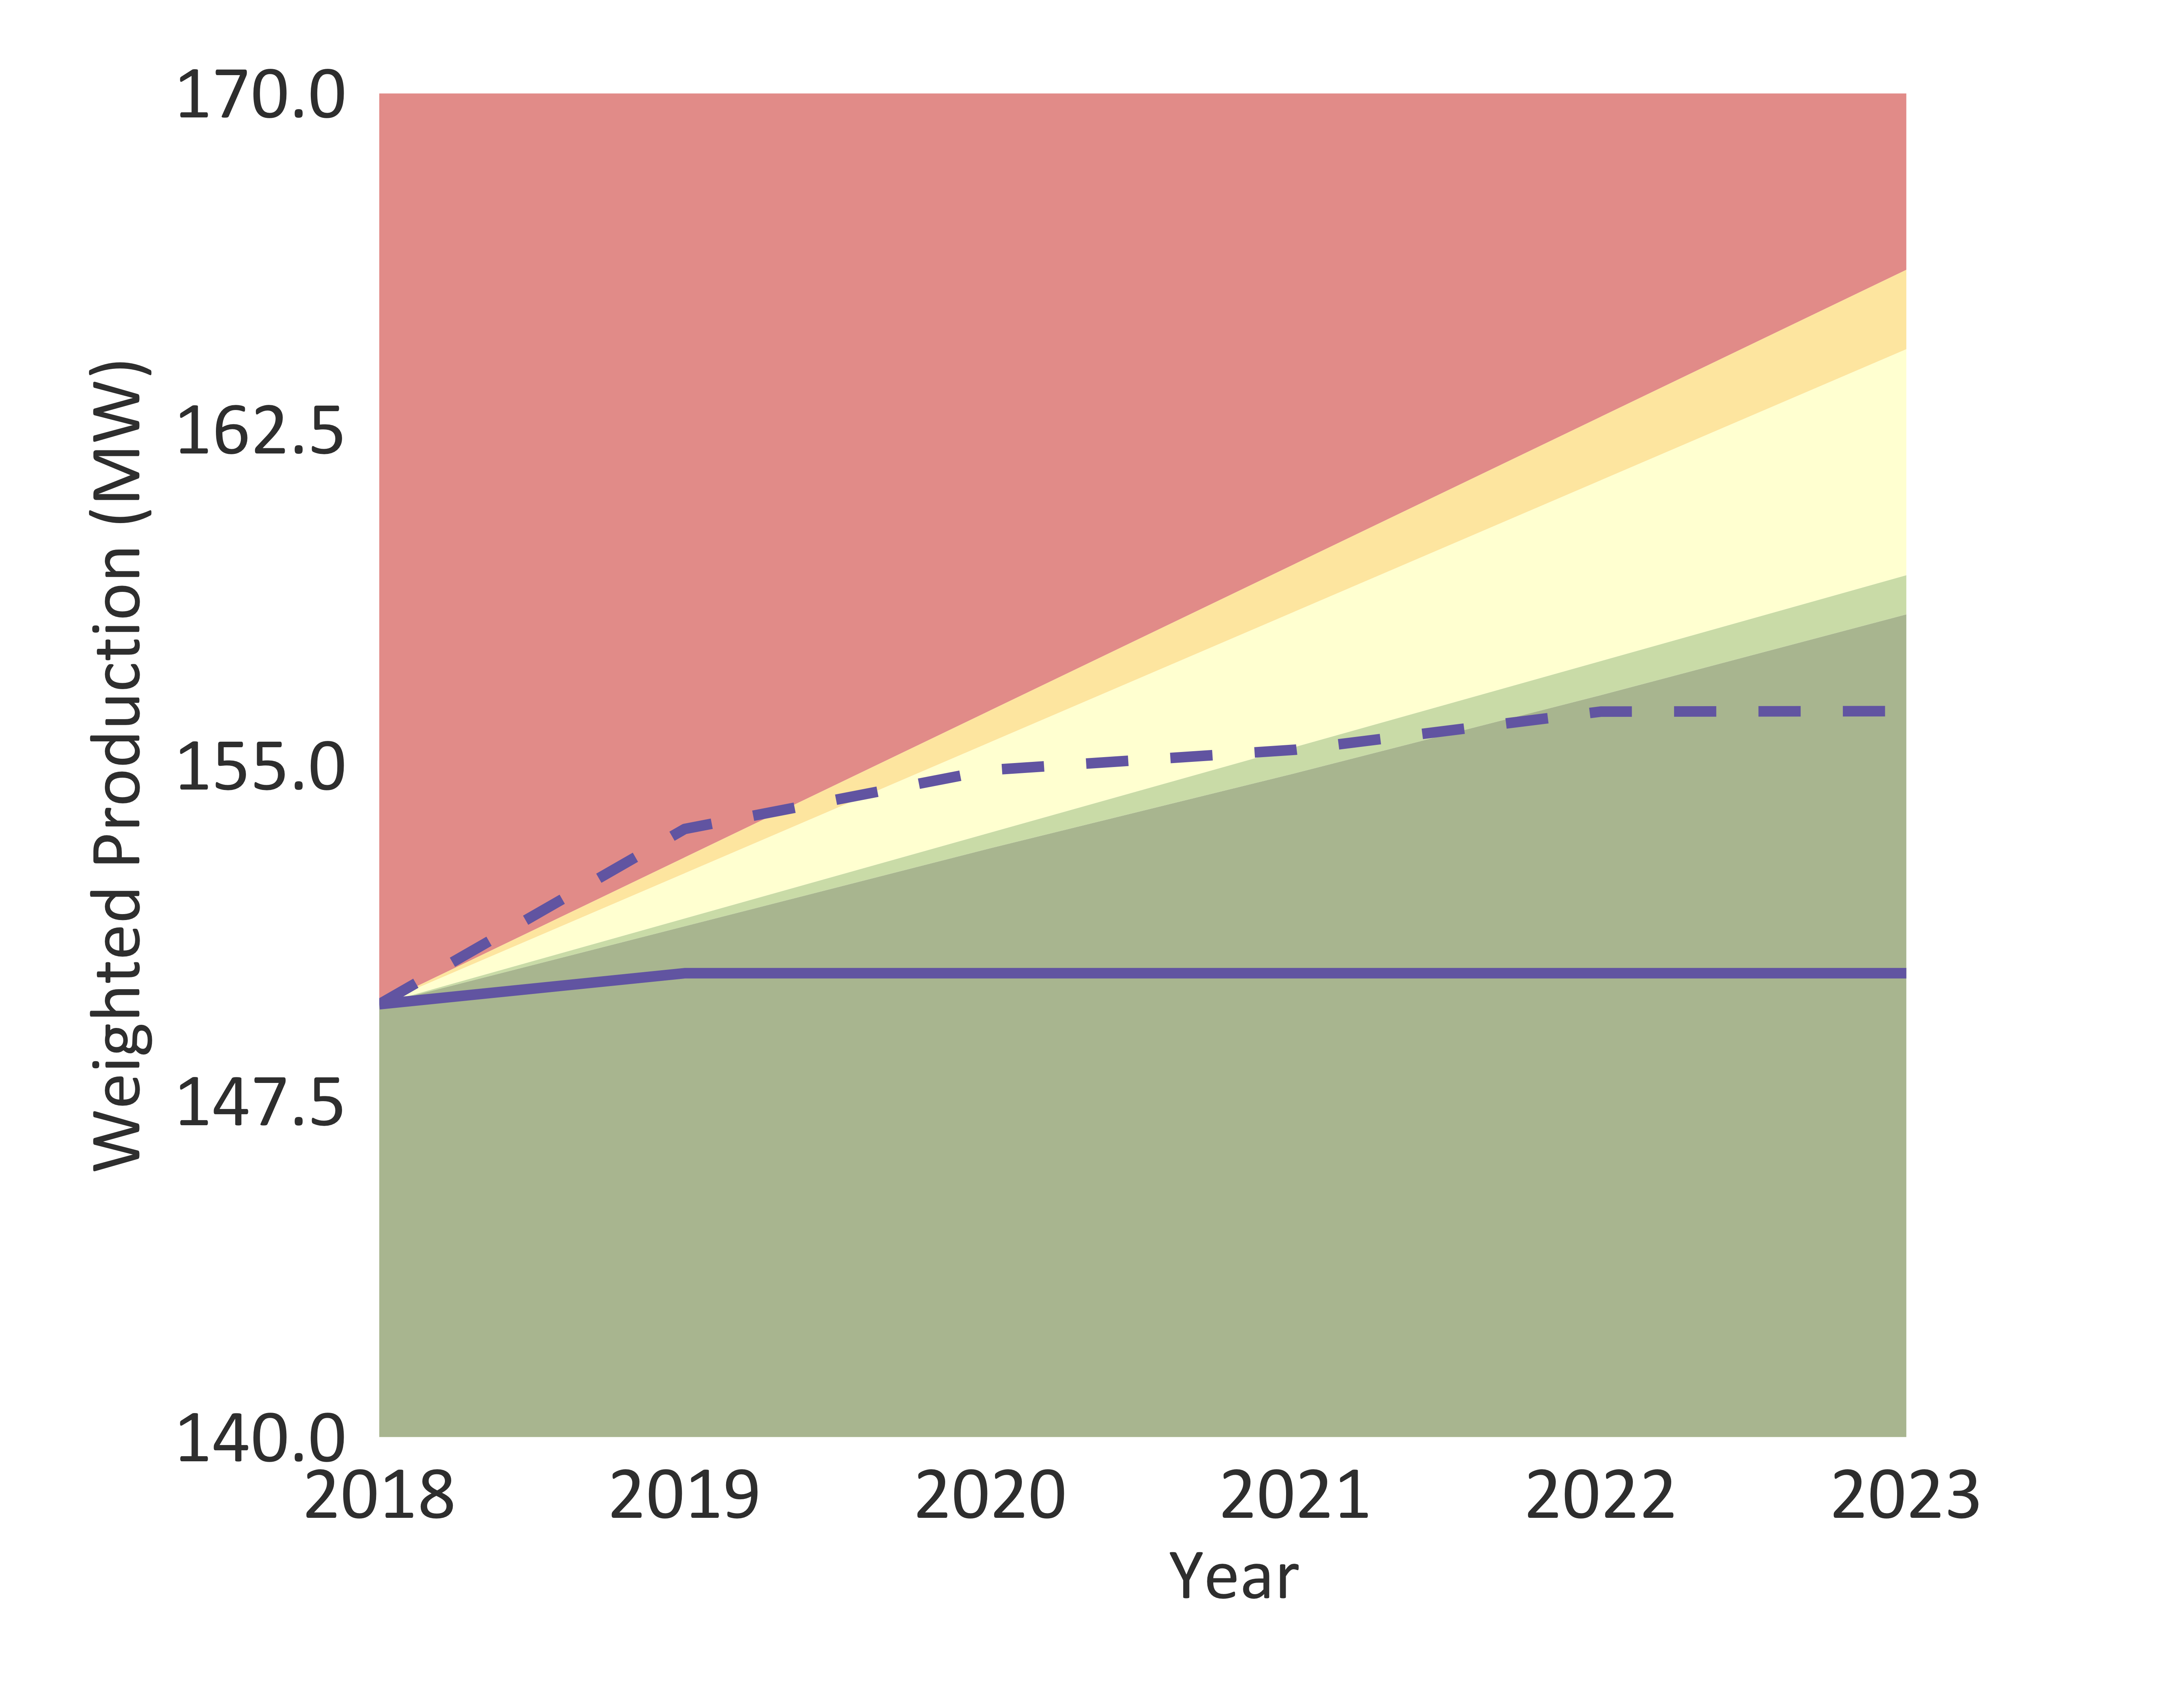
\includegraphics[trim = {0 0cm 0 0},width=1\linewidth]{CAFigures/Fig09}
	\end{center}

	\PageFooterFourth
	\newpage 

	
	\section*{} % 5th SECTION   
	\SectionHeading{SECTION 5:}{PHYSICAL RISK}
	
	\newpage
	\section*{} %
	\HeaderSingle{ENVIRONMENTAL RISK EXPOSURE 2020}
	
	\begin{multicols}{2}
		
		\textbf{Physical climate risks have been identified by financial regulators and insurance companies as a major financial risk to portfolios.}
		
		The Network for Greening the Financial System (NGFS), a global network consisting of 19 central banks and supervisors, argues for immediate action:
		
		\textit{``Exact pathways may be uncertain but it is foreseeable that financial risks will crystallize in some form through either the physical or transition channel, or some combination of them both. And while the financial risks may be realized in full over extended time horizon, the risks call for action in the short-term to reduce impact in the long-term.”}
		
		Scenario analysis regarding physical climate risks also constitutes one of the core recommendations of the Financial Stability Board Task Force on Climate-related Financial Disclosures (TCFD). 
		
		\textbf{Physical risks can impact companies' cash flows and by extension the prices of financial securities and value of financial portfolios through three channels:}
		
		\textbf{Direct effects} are those effects by which physical risks directly impact the operational and / or production capacity of a company. Direct effects are usually measured at the point of production (e.g. power plant, factory, steel plant, etc.). However, they could also arise if the headquarters of a company are impacted, thus inhibiting a company’s ability to manage and control remote production processes. 
		
		\textbf{Market effects} are indirect effects by which a company’s markets are impacted by direct physical risks, thus inhibiting the company’s ability to sell into these markets. Market effects may arise as a result of damages to transport infrastructure inhibiting supply (e.g. damages to ports, electricity transmission lines, etc.) or consumers purchasing power inhibiting demand (e.g. a hurricane damaging coastal communities).
		
		\textbf{Domino effects} are knock-on effects from market effects or other factors that inhibit cash flows. These could lead to a diversion of resources to damaged communities that were originally earmarked for purposes benefitting the company. They could also lead to economic knock-on effects where a collapse in demand in one market impacts a second market that the company has significant exposure to. In that vein, transition risks can be considered ‘domino effects’ as climate policy accelerates in response to extreme weather events. 
		
		\textbf{Each of these risks can impact cash flows in one of two ways:}
		
		Physical risks can create \textbf{one-off impacts} after which productive capacities and markets recover. These types of risks can manifest themselves through losses in cash flows in the short-term as well as through ‘recovery costs’ and additional adaptation costs;
		
		Alternatively, physical risks can give rise to \textbf{permanent impacts} on cash flows with no recovery or adaptation costs, but more long-term impacts in terms of lost cash flows.
		
		\textbf{Given the relatively nascent nature of physical climate risk modeling, the scenario analysis in this report will be limited to an `exposure’ perspective based exclusively on direct effects.}
		
		
	\end{multicols}
	
	\PageFooterFifth
	\newpage
	\section*{} %
	\HeaderSingle{ENVIRONMENTAL RISK EXPOSURE 2020}
	
	
	\begin{multicols}{2}
		\textbf{Climate-related physical risks cut across a range of traditional natural disaster categories (EM-DAT 2016):}
		
		\textbf{Climatological risks} arise from hazards related to long-lived, meso- to macro-scale atmospheric processes ranging from intra-seasonal to multi-decadal climate variability. Notable examples are droughts and wildfires. Climatological risks – as the name suggests – are likely to increase significantly in the medium- to long-term under global warming.
		
		\textbf{Meteorological risks} arise from hazards caused by short-lived, micro- to meso-scale extreme weather and atmospheric conditions that last from minutes to days (e.g. storms, hurricanes). These events are similarly likely to intensify over time, with some evidence that the frequency and severity of hurricanes is likely to accelerate as a result of global warming.
		
		\textbf{Hydrological risks} arise from hazards caused by the occurrence, movement, and distribution of surface and subsurface freshwater and saltwater (e.g. floods). Sea level rise resulting from glacier melting has been noticeable over the past two decades and is likely to increase over time.
		
		\textbf{Geophysical risks} arise from hazards originating from solid earth. This term is used interchangeably with the term geological hazard. Examples include earthquakes or tsunamis. There is some academic literature suggesting that the impacts of climate change increase seismic activity (Sauber and Ruppert 2008).
		
		\textbf{Biological risks} arise from hazards caused by exposure to living organisms and the toxic substances (e.g. venom, mold) or vector-borne diseases that they may carry. Changes in climate are likely to reduce biodiversity (SOURCE), which may be critical for e.g. agricultural activities.
		
		In this scenario analysis report, the focus will be on three types of physical climate risks across the areas described above: i) droughts, ii) floods, and iii) wildfires.
		
		
	\end{multicols}

	\begin{multicols}{2}
		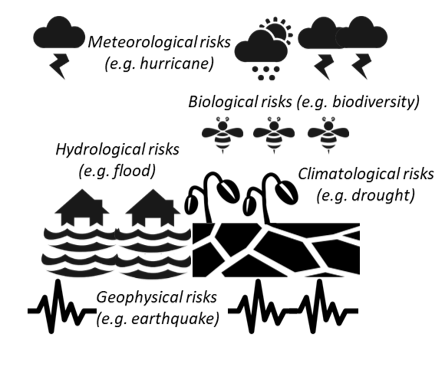
\includegraphics[width=1\linewidth]{ReportGraphics/PhysicalClimateRisks.png}
		
		\textbf{\small Overview of physical climate risks (Source: Authors)}
	
		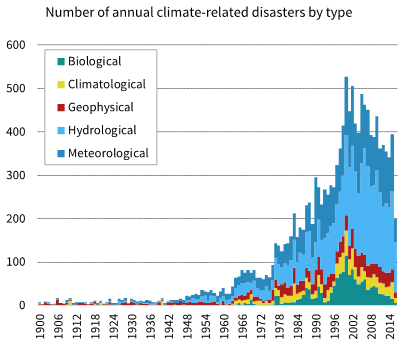
\includegraphics[width=1\linewidth]{ReportGraphics/ClimateDisasters.png}
		
		\textbf{\small Annual climate-related disasters by type (Source: Authors, based on EM-DAT)}
	\end{multicols}

	\PageFooterFifth
	\newpage
	\section*{} %
	\HeaderDouble{ENVIRONMENTAL RISK EXPOSURE}{WATER STRESS 2020 \& 2040}
	
	\begin{multicols}{2}
		\textbf{The figures below show the percent exposure to water stress of thermal power plants in the corporate bond and listed equity portfolios, based on the WRI Aqueduct risk map in 2030.}
		
		Water stress as a physical risk is a particular challenge for thermal power plants, which are labelled here as coal, oil, nuclear, and gas power plants \textit{(note: Technically, solar thermal and geothermal power plants also fall in this category, though they operate differently relative to water stress)}. This physical risk should be distinguished from flood risk, which is explored in more detail on the next page.
		
		The charts show, for each asset class, the current asset base exposure to water stress in 2020 and 2030, as well as the distribution of that exposure across individual corporate bonds in the relevant portfolio in 2030 only. Risk levels are defined in four categories: 'extremely high and arid' refers to water stress with projected ratios of water withdrawal to supply exceeding 80\%, 'high' refers to projected ratios from 40-80\%, 'middle-low' refers to projected ratios from 0-40\%, while 'unknown' refers to unmapped assets that could not be linked to a risk category. See the ANNEX for additional information on risk categories.
		
	\end{multicols}

	\textbf{Water stress risk levels for thermal power assets. Each bar represents a single bond and stock, respectively. }
	
	%PowerSector_CBS
	\textbf{Bond portfolio}
	
	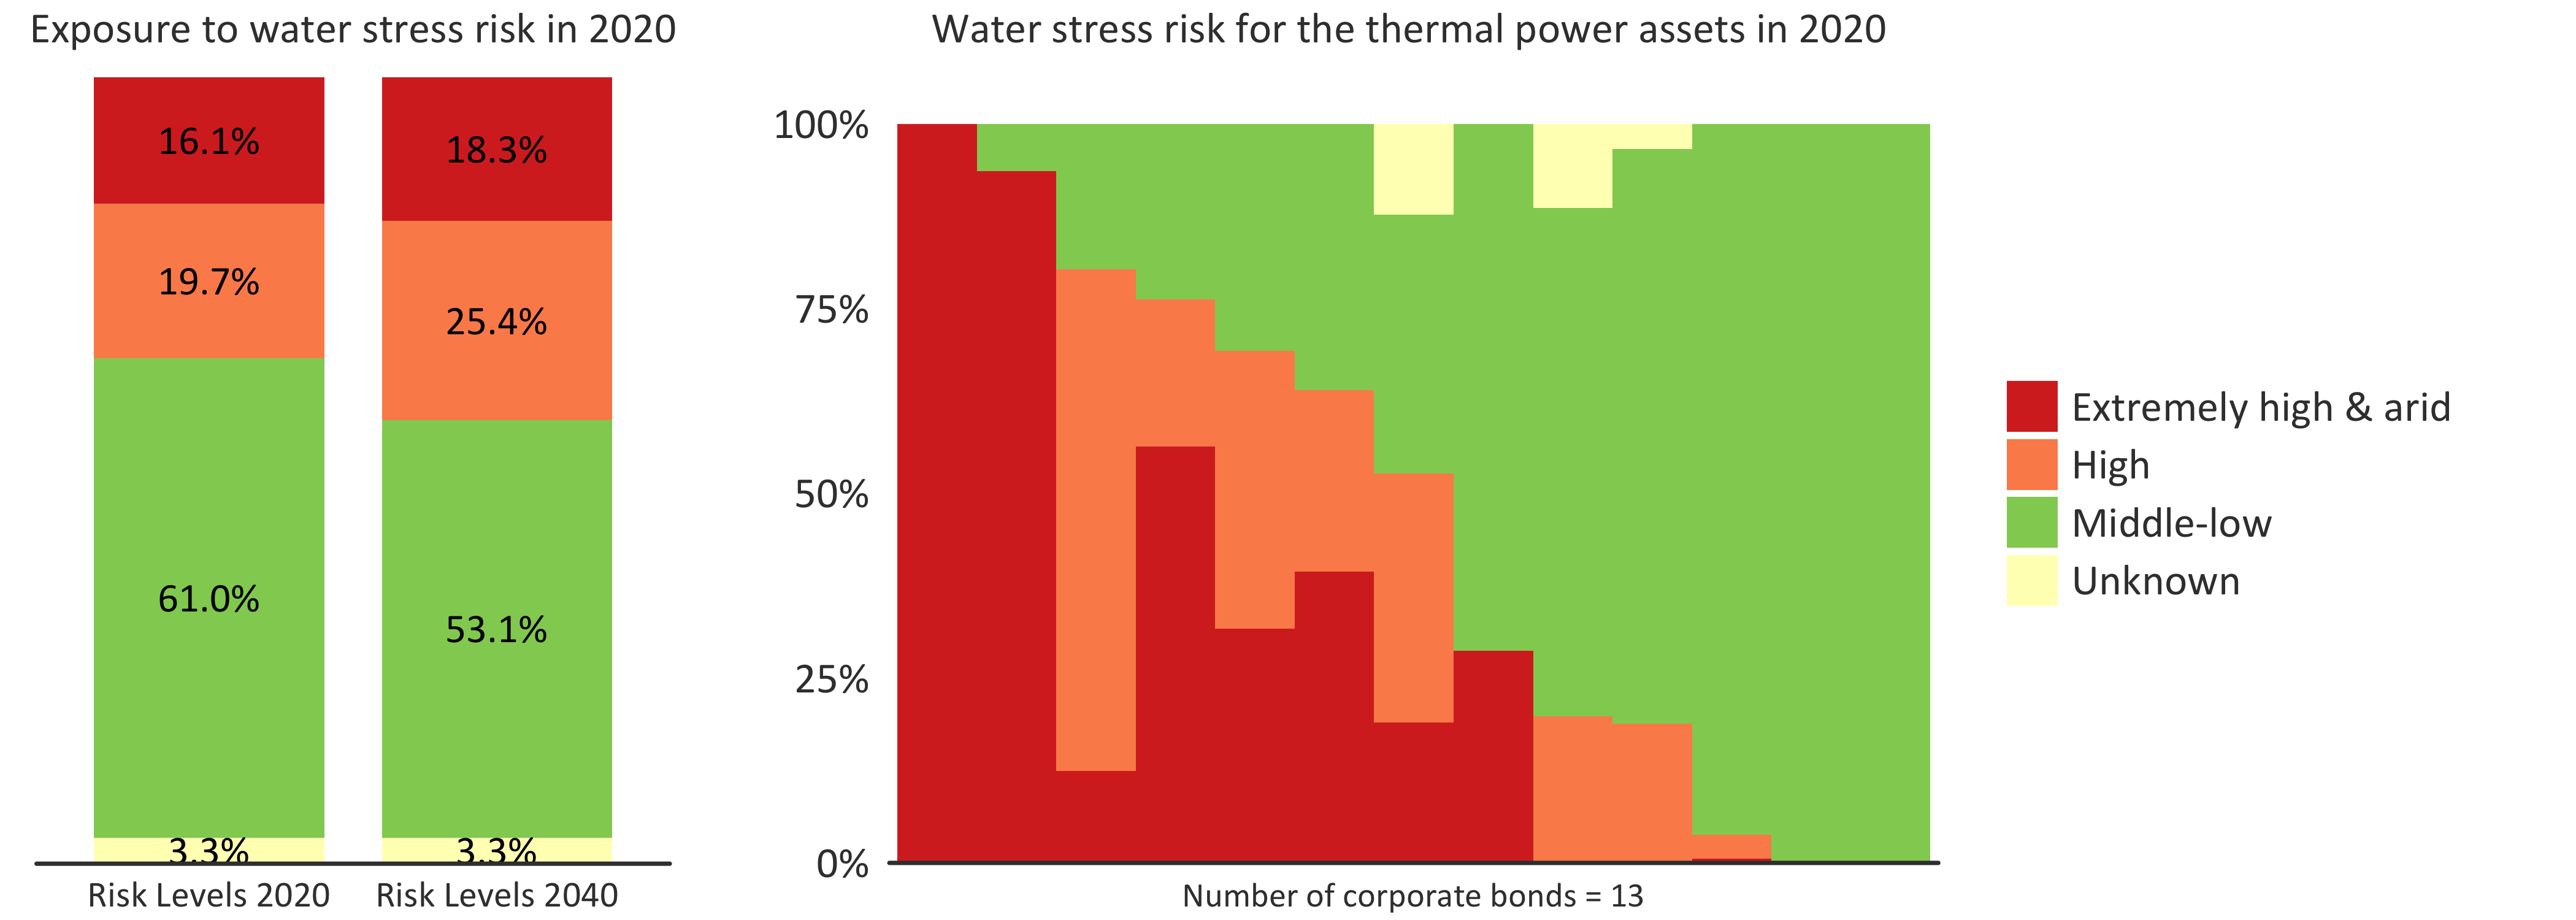
\includegraphics[width = 1\linewidth]{CAFigures/Fig70}
	%PowerSector_CBE

	%PowerSector_EQS
	\textbf{Equity portfolio}
	
	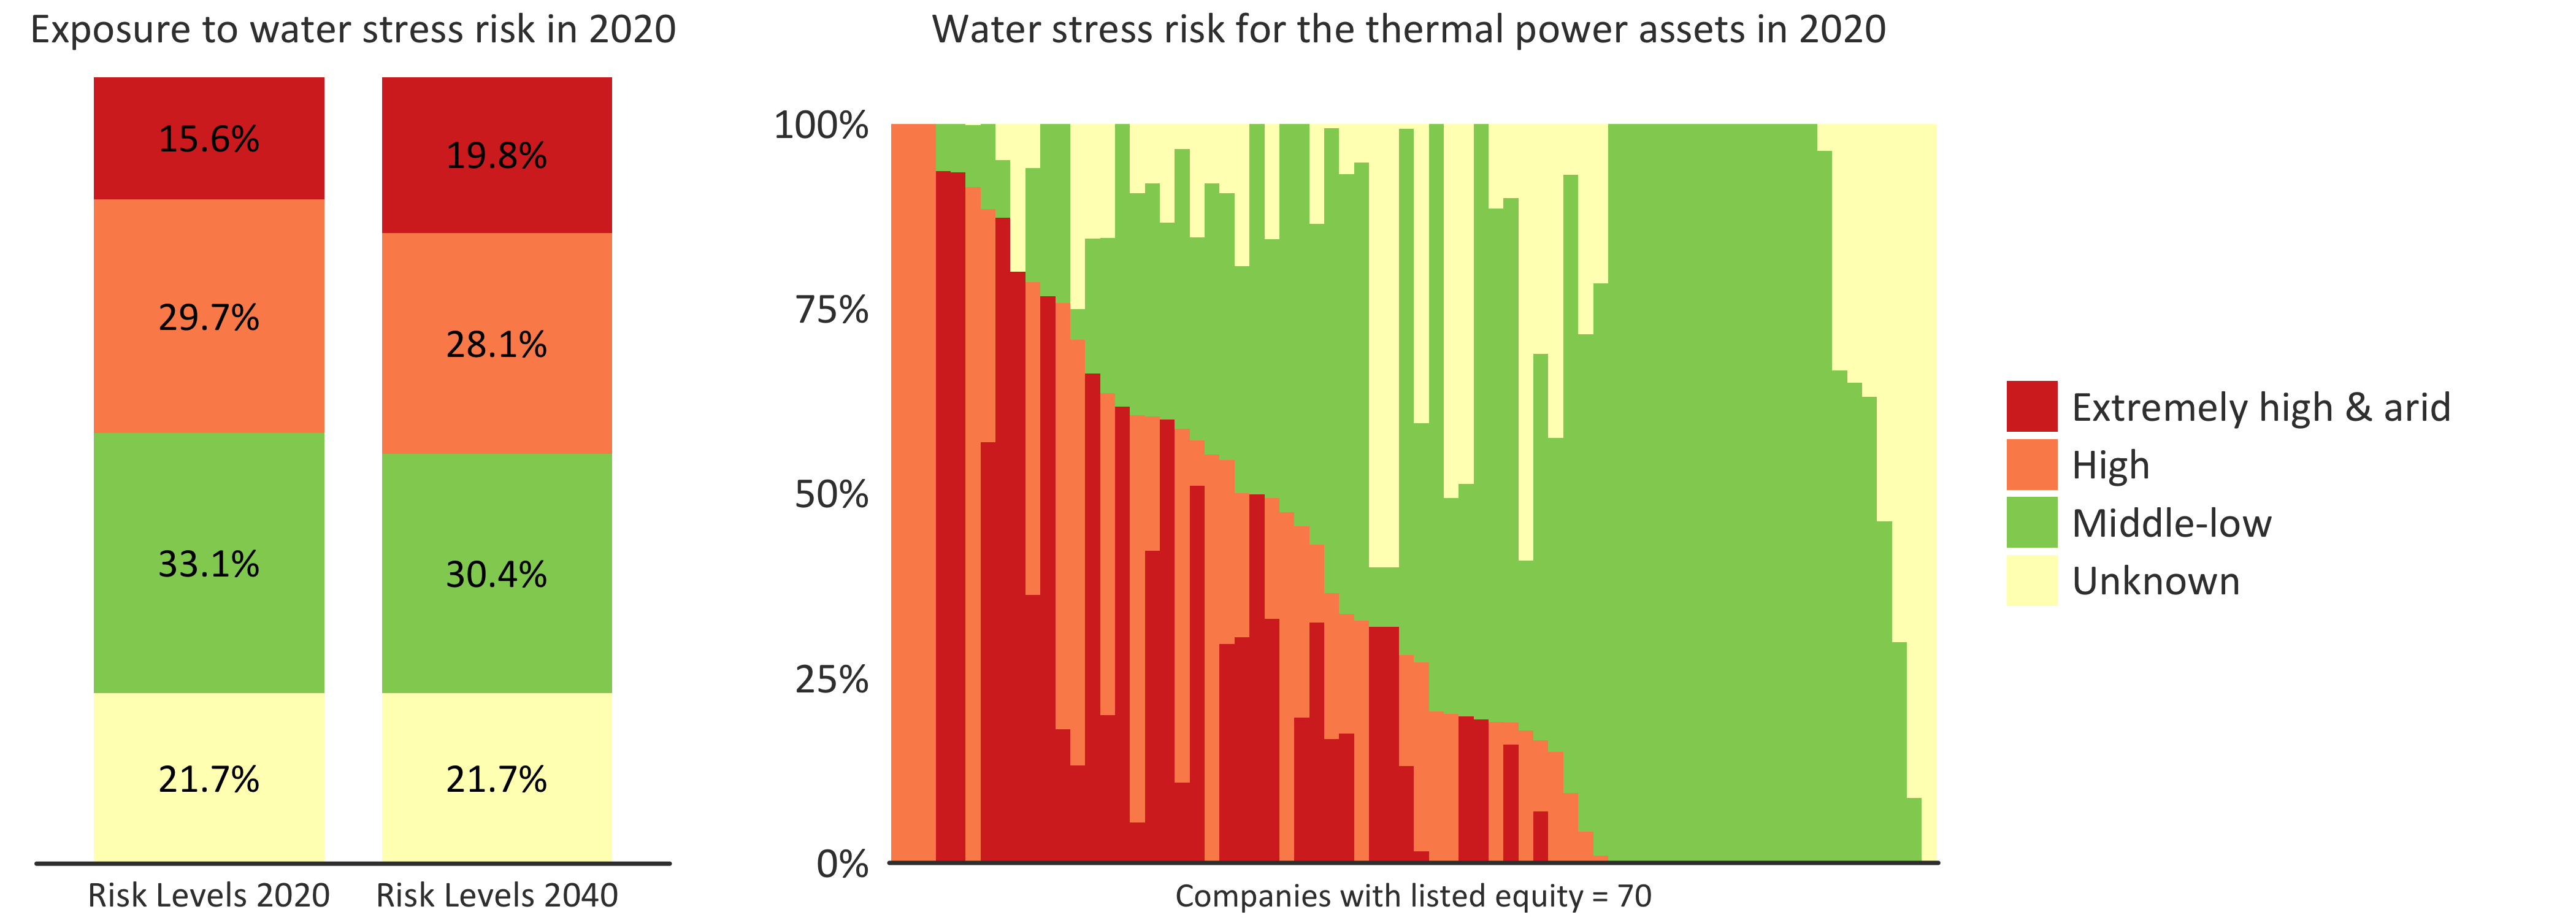
\includegraphics[width= 1\linewidth]{CAFigures/Fig71}
	%PowerSector_EQE
	
	\PageFooterFifth
	\newpage
	\section*{} %
	\HeaderDouble{ENVIRONMENTAL RISK EXPOSURE}{FLOOD AND WILDFIRE}

	\begin{multicols}{2}
		\textbf{The analytics below summarize the exposure of the portfolios’ power assets, oil and gas assets, and coal mining assets to flood and wildfire risk.} 
		
		The flood risk analytics build on an EU-developed global flood risk map that classifies flood risk as 1 in 10, 1 in 20, 1 in 100, 1 in 200, or 1 in 500. The analysis here uses the 1 in 100 scenario, assuming an increased likelihood of flood events in a climate scenario. 
		
		The actual degree of `flood risk’ is a function of the specific nature of the asset and its position. Thus, a 2 meter flood may be material for some types of assets and not for others. As a result, the actual risk classification – being generic – may not be reflective of the actual underlying risk to any individual asset. As such, the classification seeks merely to represent the exposure of the portfolios’ assets to various flood outcomes.
		
		The wildfire risk analytics build on the UNEP global wildfire risk map. Similar to flooding, wildfire risk will not constitute an equal ‘threat’ to all types of assets, varying in prominence as a function of specific characteristics of the assets. 
		
		Risk levels are defined in three categories: risk, no risk, and unknown. In the flood charts, `risk' refers to any flood height exceeding 0 meters, `no risk' refers to a flood height of 0 m, and 'unknown' refers to assets that could not be linked to flood height figures. In the wildfire charts, `risk' refers to an event density of at least 1 day (per year), `no risk' refers to an event density of 0 days, and 'unknown' refers to assets that could not be linked to event density figures. See the ANNEX for additional information on risk categories.
		
		
	\end{multicols}
	
	\textbf{Percent exposure of power, oil and gas, and coal mining assets to flood and wildfire risk in 2020 for A) corporate bonds and (B) listed equity stocks. }
	
	%PhysicalRisk_Fire_CBS
	\textbf{Bond portfolio}
	\begin{multicols}{2}
		
		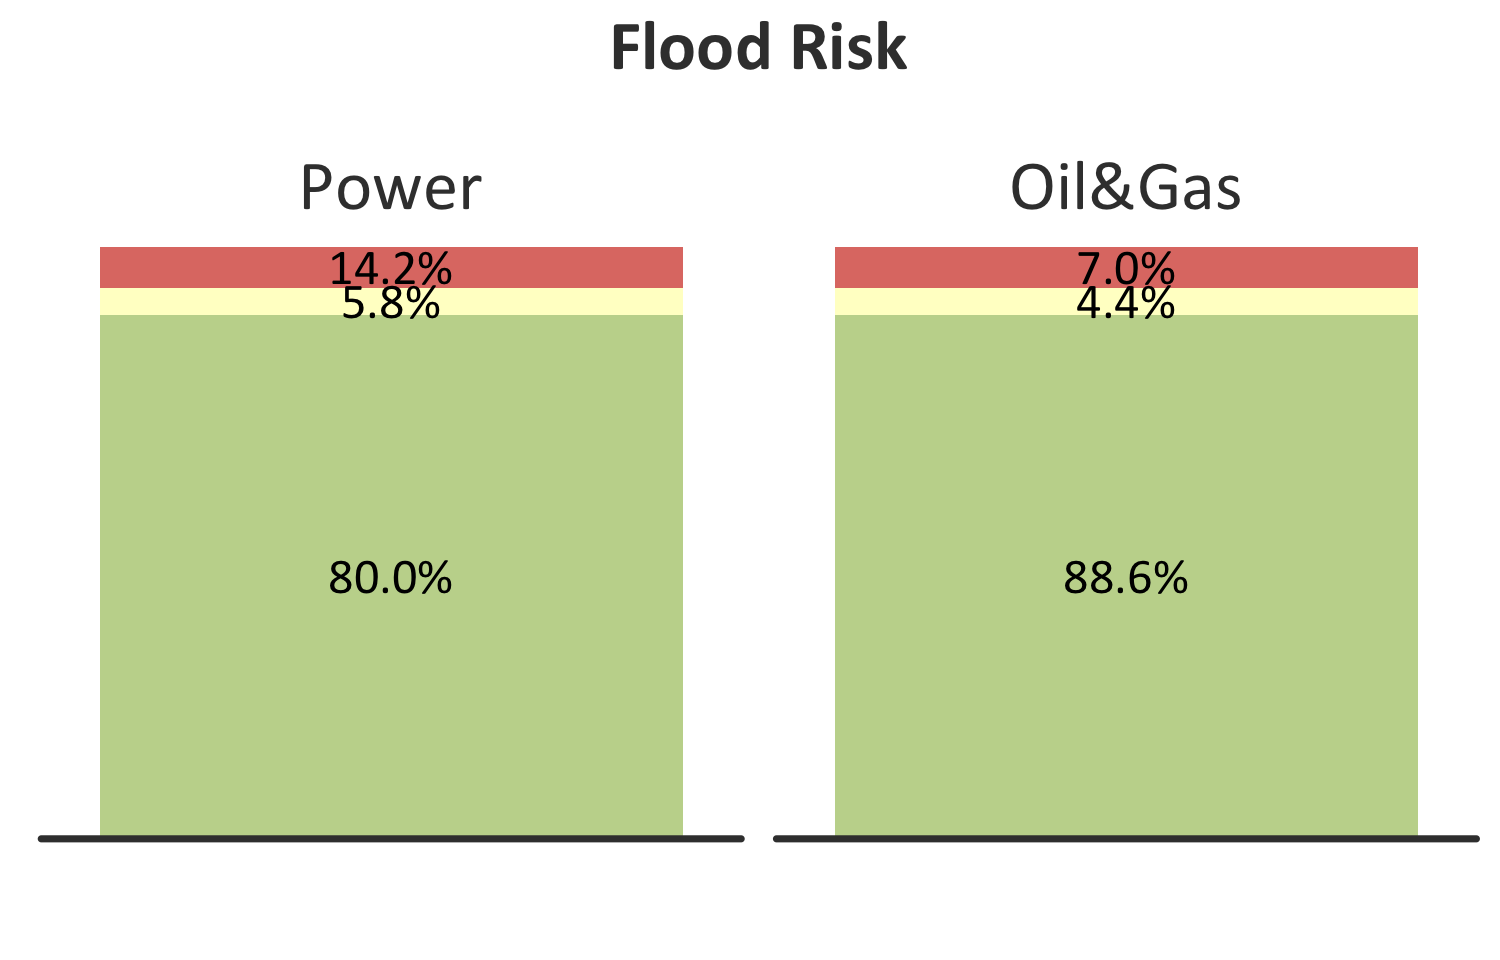
\includegraphics[width = 1\linewidth]{CAFigures/Fig72}
		
		
		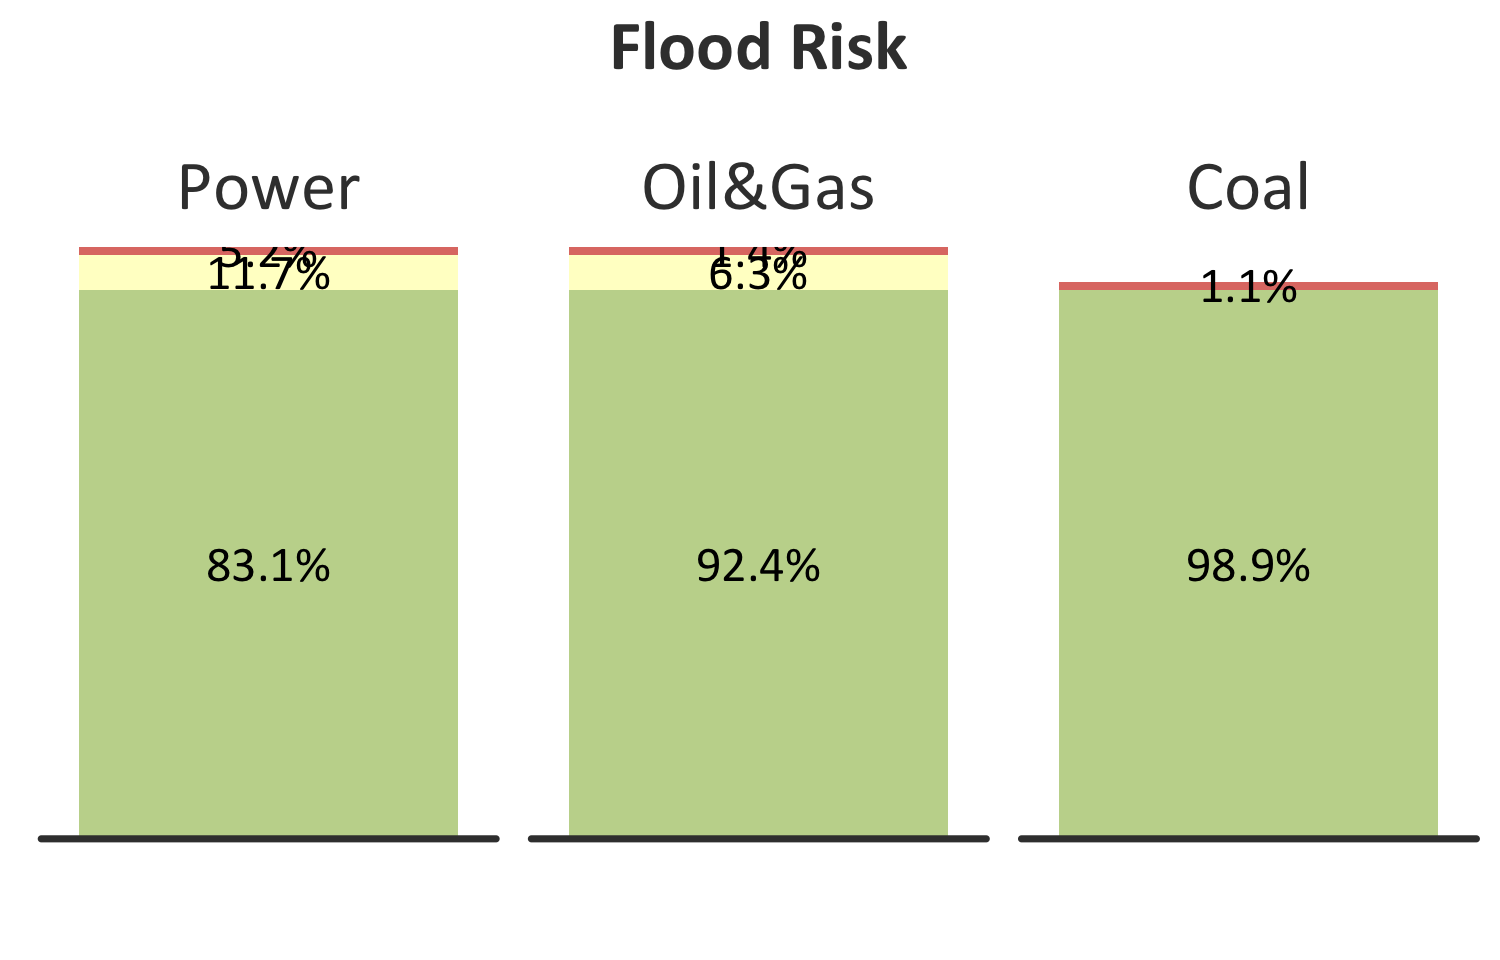
\includegraphics[width = 1\linewidth]{CAFigures/Fig73}
	\end{multicols}
	%PhysicalRisk_Fire_CBE
	
	%PhysicalRisk_Fire_EQS
	\textbf{Equity portfolio}

	\begin{multicols}{2}
		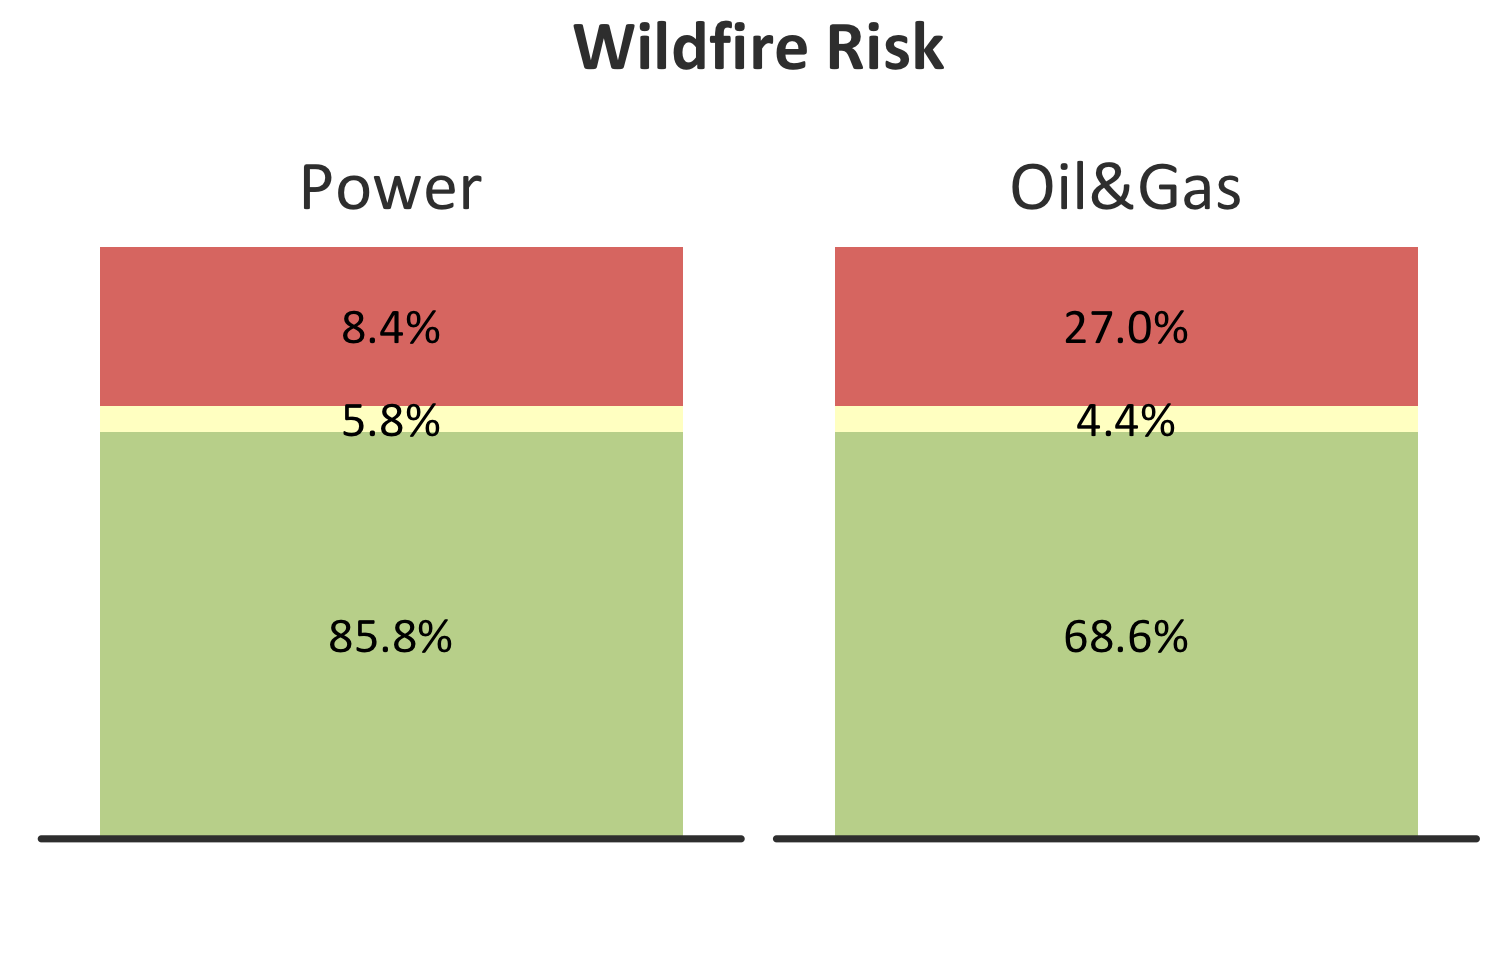
\includegraphics[width = 1\linewidth]{CAFigures/Fig74}
		
		
		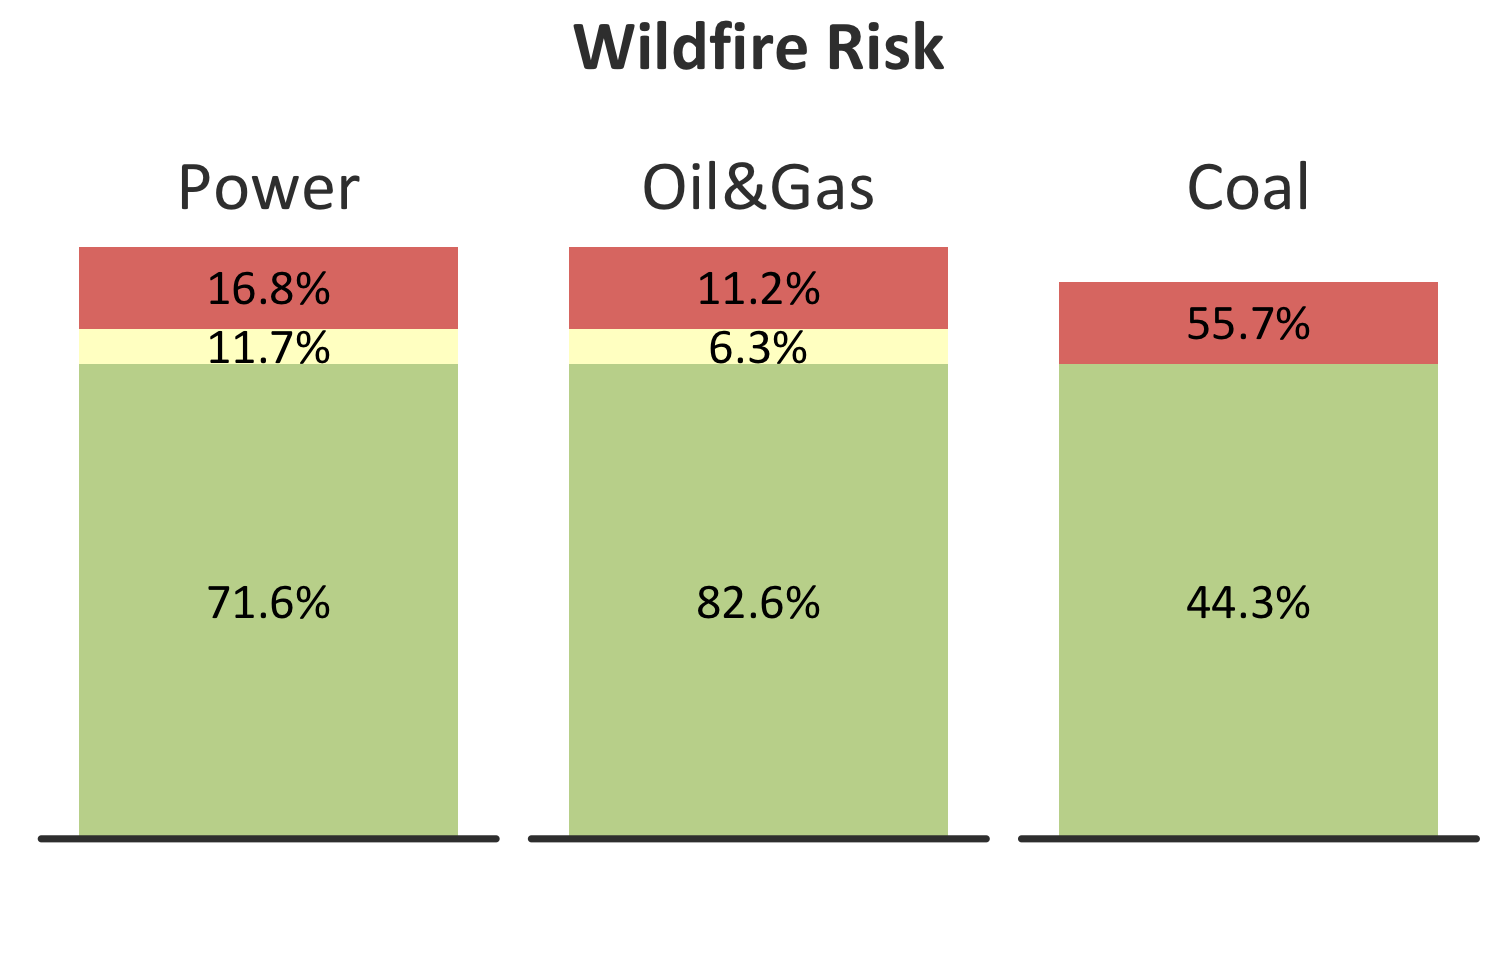
\includegraphics[width = 1\linewidth]{CAFigures/Fig75}
	\end{multicols}
	%PhysicalRisk_Fire_EQE
	
	\PageFooterFifth
	\newpage	
	\section*{} % 6th SECTION   
		\SectionHeading{SECTION 6:}{COMPANY EXPOSURE}
		
		\newpage
	\section*{} % CONTRIBUTIONS OF SECURITIES TO THE RESULTS   %CompanyChartsS
	\HeaderSingle{CONTRIBUTIONS OF SECURITIES TO THE RESULTS}
	
	\begin{multicols}{2}
		
		\textbf{The objective of this section is to provide insight into the specific companies driving the
			results presented in the previous sections.}
		
		The following pages will show results for individual companies in the fossil fuel, power, and automotive sector. The analytics provided show just one piece of information related to potential scenario analysis of companies and their contribution to a portfolio's performance. A range of additional indicators could be considered that go beyond the scope of this particular report. As a result, the indicators presented here should not be understood as providing investment recommendations, but rather as a summary of the exposures of the companies that are driving the results of the portfolio scenario analysis. Section 6 provides further detail on the data sources informing this section. 
		
		As part of a partnership with a range of technical experts, the 2° Investing Initiative is currently developing a company scenario analysis report mirroring the portfolio reports presented here, designed to be made freely available and provide a more comprehensive and holistic picture of a company's positioning relative to a decarbonization scenario. This infrastructure can be used to inform future scenario analysis and actions and will be launched in the second half of 2018. The analytics in this report thus only show a snapshot of the type of data that can be explored. 
		
		The following will briefly summarize the type of data that will be shown for each sector. 
		
		\textbf{Oil and gas.} For oil and gas production, three types of indicators will be shown. The first indicator is the total planned change in production of oil and gas companies over the next 5 years, based on their currently revealed production plans from the asset-level databases. The graphs on the next page show the largest companies by amount of oil or gas production allocated to the fixed income and equity portfolios in 2018; these companies have the most influence on the portfolio's alignment results for the fossil fuels sector. For each asset class and technology, the results are shown relative to the portfolio's targeted total change in production during the 5 year period under the 2° scenario (green bar). It should be noted that the figures provided are based on current estimated production and evolution of the existing asset base.  Mergers, acquisitions, and increases in capital expenditure relative to baselines may of course lead to changes in these trends over time. 
		
		The second indicator builds on analysis conducted by the Carbon Tracker Initiative in partnership with the UN Principles for Responsible Investment (UNPRI). This indicator takes a more long-term view and analyses the alignment of companies with a 2°C carbon budget from the perspective of the cost structure of their oil and gas assets. This indicator differs from the first in terms of the time horizon and the underlying allocation rules that allocate macro scenarios to microeconomic actors. More information on the methodology and the approach can be found at http://www.2degreeseparation.com/. This indicator can only be used to analyze the listed equity portfolio, as data is unavailable for fixed income securities.
		
		Finally, the third indicator shows the breakdown of oil assets of individual companies by type of oil (e.g., conventional, tar sands, etc.). Wood Mackenzie (2018) proposes that while shifting away from high-carbon fuels towards low carbon is necessary as an overall trend, within the oil and gas industry, shifting away from particular extraction methods is a transitional alternative. This report does not comment on the emissions by extraction type, however data is available on this. Investors need to look beyond resource themes and review the variations in upstream emissions intensity to see how companies can reduce their carbon footprints. Even assets of the same theme can have significantly different emissions intensity based upon maturity, location and other unique factors.
		
		\textbf{Power and automotive sectors.} For the power and automotive sectors, the company level information focuses on the technology mix of the utilities and automotive manufacturers in the fixed income and equity portfolios, informing in particular the results for Section 4. Additional information on the build out plans of these companies and the changes over time can be provided upon request. 
		
		
	\end{multicols}
	
	\PageFooterSixth
	\newpage
	\section*{} % CONTRIBUTIONS OF SECURITIES TO THE RESULTS   %FossilFuelSector_ALLS
	\HeaderDouble{CONTRIBUTIONS OF SECURITIES TO THE RESULTS}{OIL AND GAS}  
	
	%FossilFuelSector_CBS
	\textbf{Planned total percent change in fossil fuel production of companies with most production allocated to the fixed income portfolio}
	\vspace{-.35cm}
	
	\begin{center}
		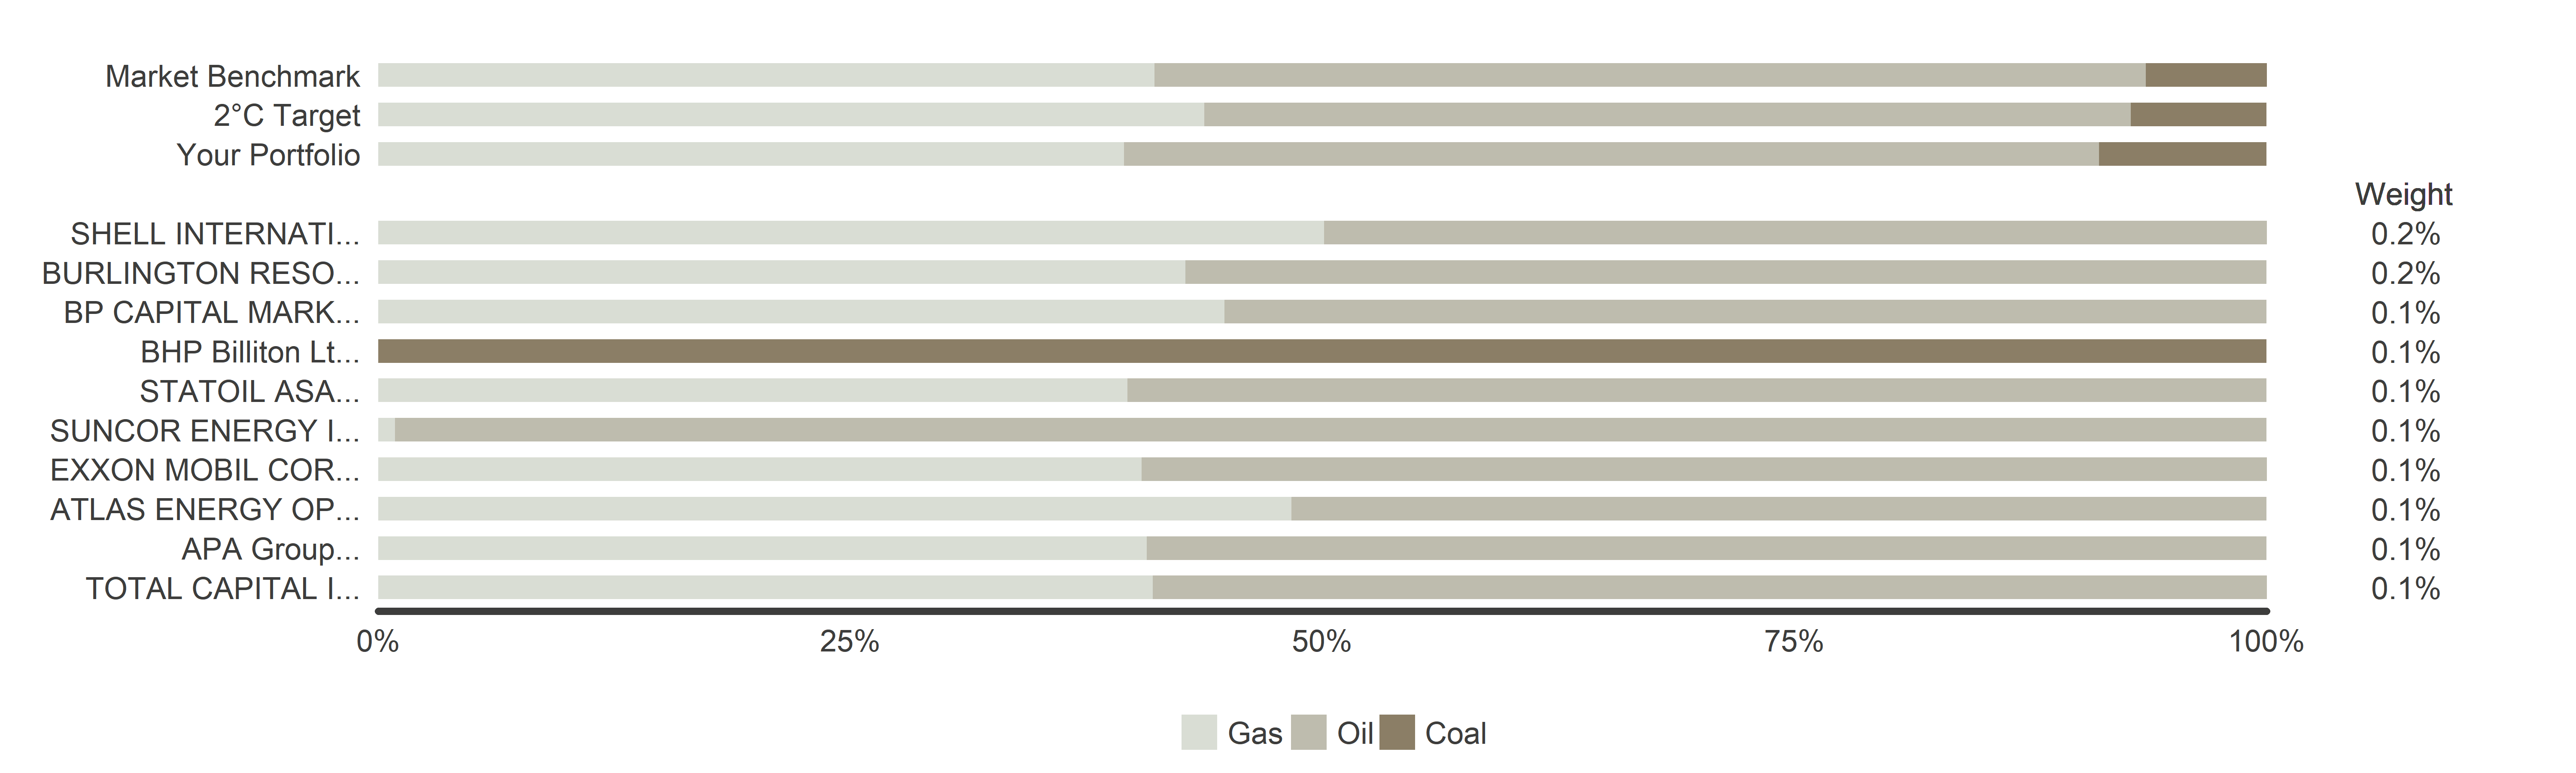
\includegraphics[trim = {0 0cm 0 0},width=1\linewidth]{CAFigures/Fig36}
	\end{center}
	%FossilFuelSector_CBE
	%FossilFuelSector_EQS
	\textbf{Planned percent change in fossil fuel production of companies with most production allocated to the equity portfolio}
	\vspace{-.35cm}
	
	\begin{center}
		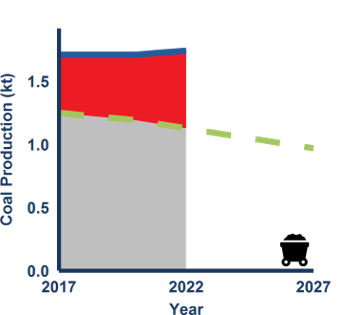
\includegraphics[trim = {0 0cm 0 0},width=1\linewidth]{CAFigures/Fig37}
	\end{center}
	\begin{center}
		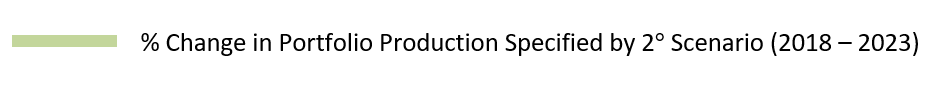
\includegraphics[trim = {0 0cm 0 0},width=.5\linewidth]{ReportGraphics/ogLegend.png}
	\end{center}
	%FossilFuelSector_EQE
	\PageFooterSixth
	\newpage
	
	\section*{} % CONTRIBUTIONS OF SECURITIES TO THE RESULTS
	\HeaderDouble{CONTRIBUTIONS OF SECURITIES TO THE RESULTS}{OIL}
	 
	
	\textbf{Carbon budget alignment of the largest oil and gas companies in the equity portfolio.} This graph is based on the work of the Carbon Tracker Initiative and UNPRI and shows the carbon budget alignment, and by extension the level of potential exposure to unneeded capex, of the largest oil and gas producers (by market value). 
	
	\vspace{-.35cm}
	
	\begin{center}
		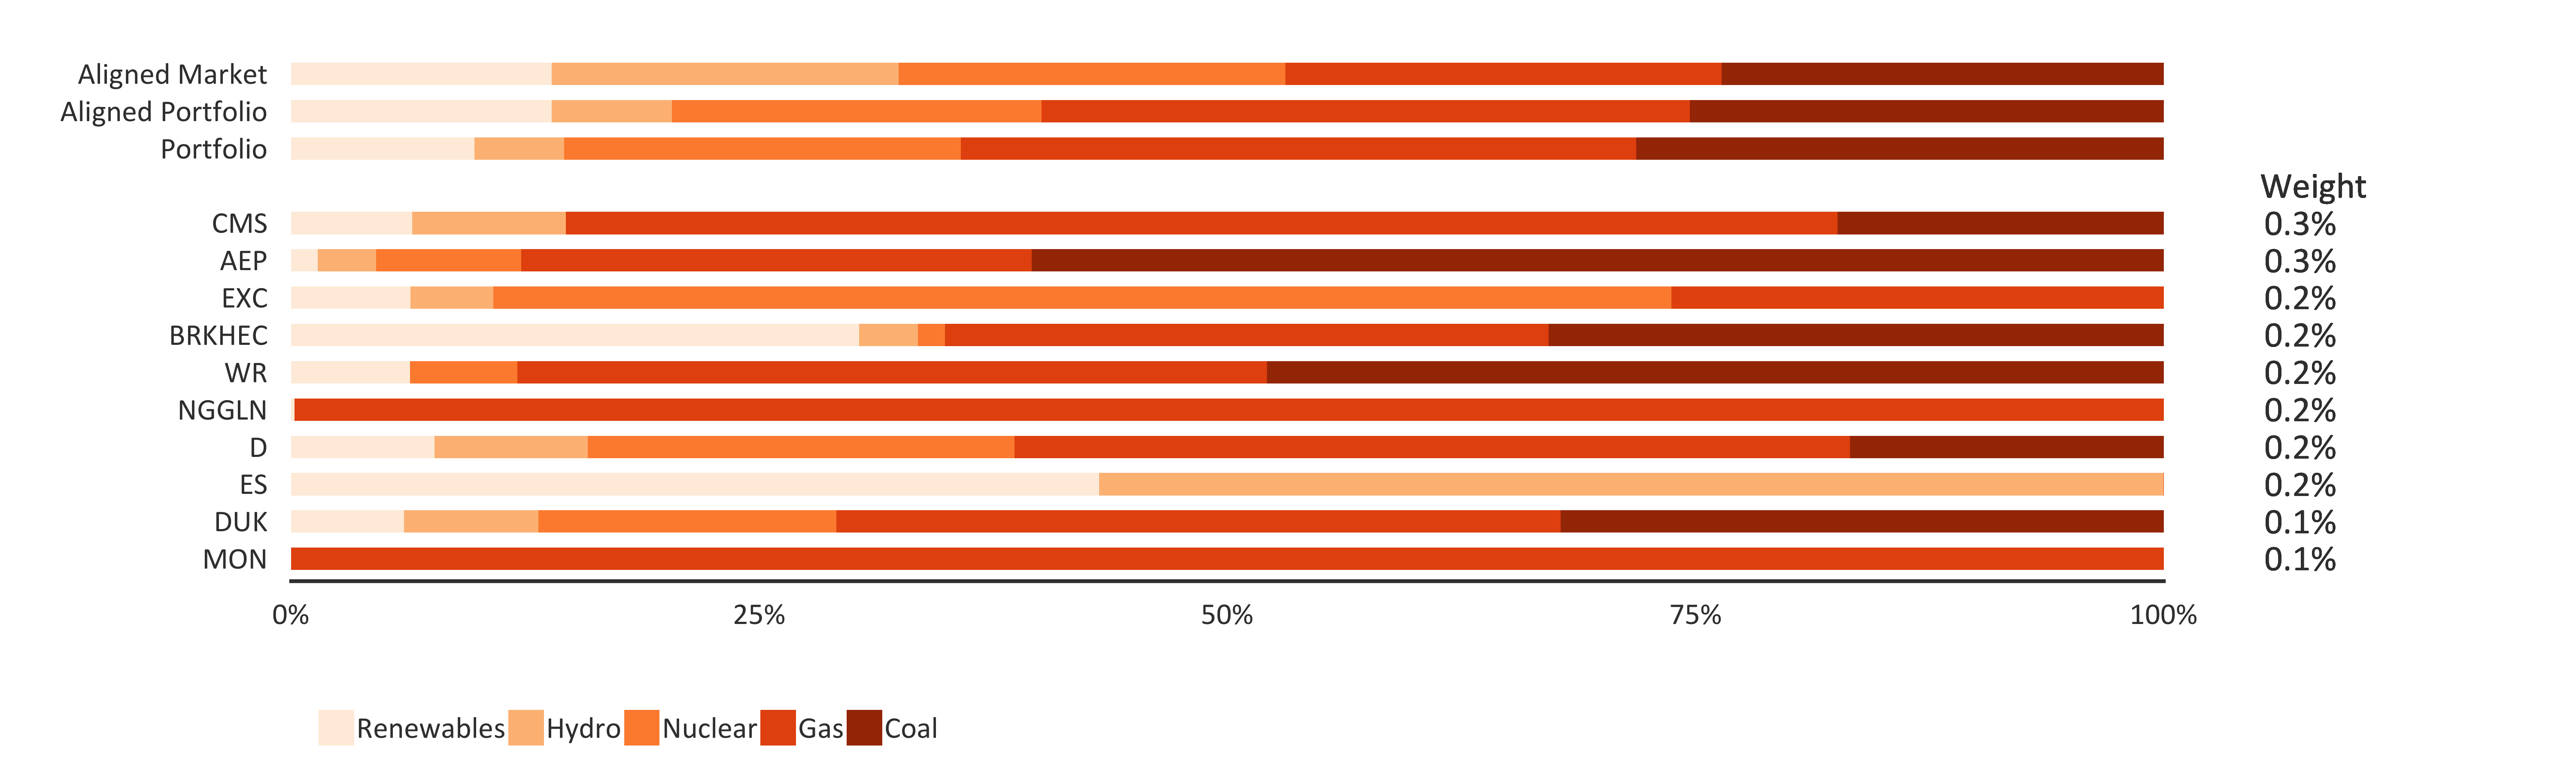
\includegraphics[trim = {0 0cm 0 0},width=1\linewidth]{CAFigures/Fig40}
	\end{center}
	
	
	
	
	\textbf{Resource breakdown of oil production of the largest holdings in the fixed income portfolio.}
	This graph shows oil production by type of oil for the largest holdings (by market value) of oil producers in the fixed income portfolio. 
	
	\vspace{-.35cm}
	
	\begin{center}
		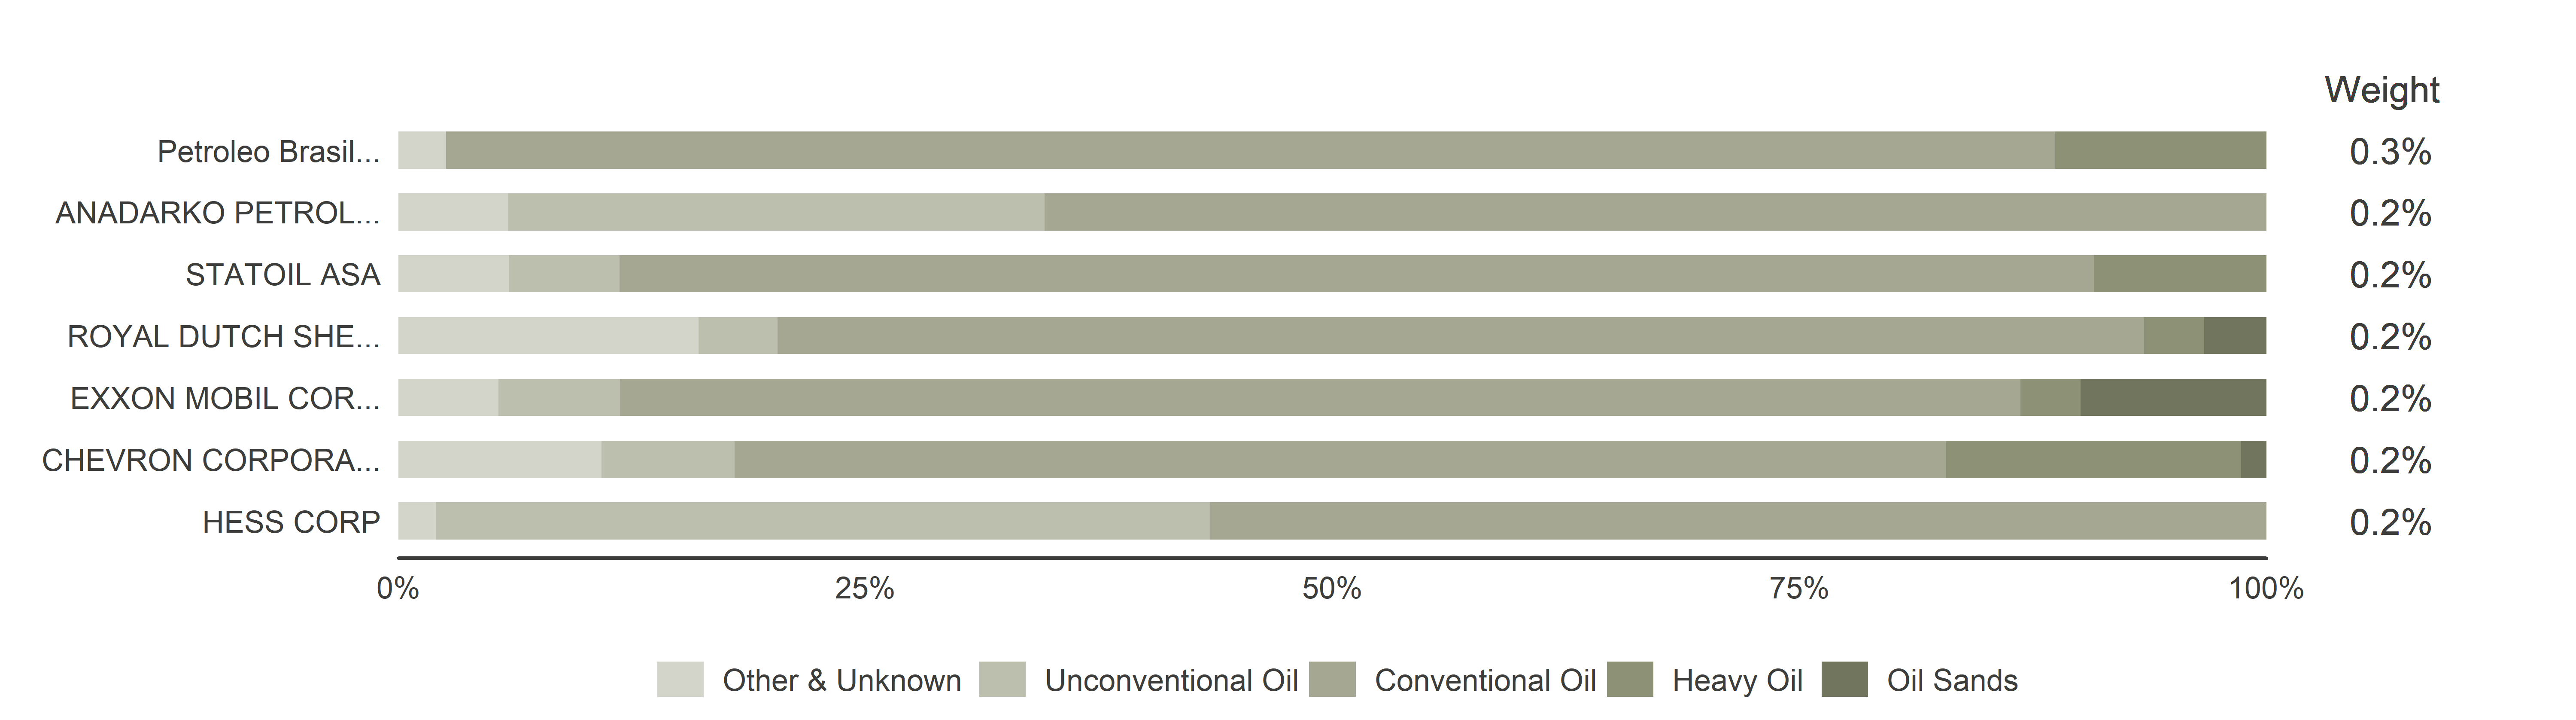
\includegraphics[trim = {0 0cm 0 0},width=1\linewidth]{CAFigures/Fig38}
	\end{center}
	
	
	
	\textbf{Resource breakdown of oil production of the largest holdings in the equity portfolio.}
	This graph shows oil production by type of oil for the largest holdings (by market value) of oil producers in the equity portfolio. 
	
	\vspace{-.35cm}

	\begin{center}
		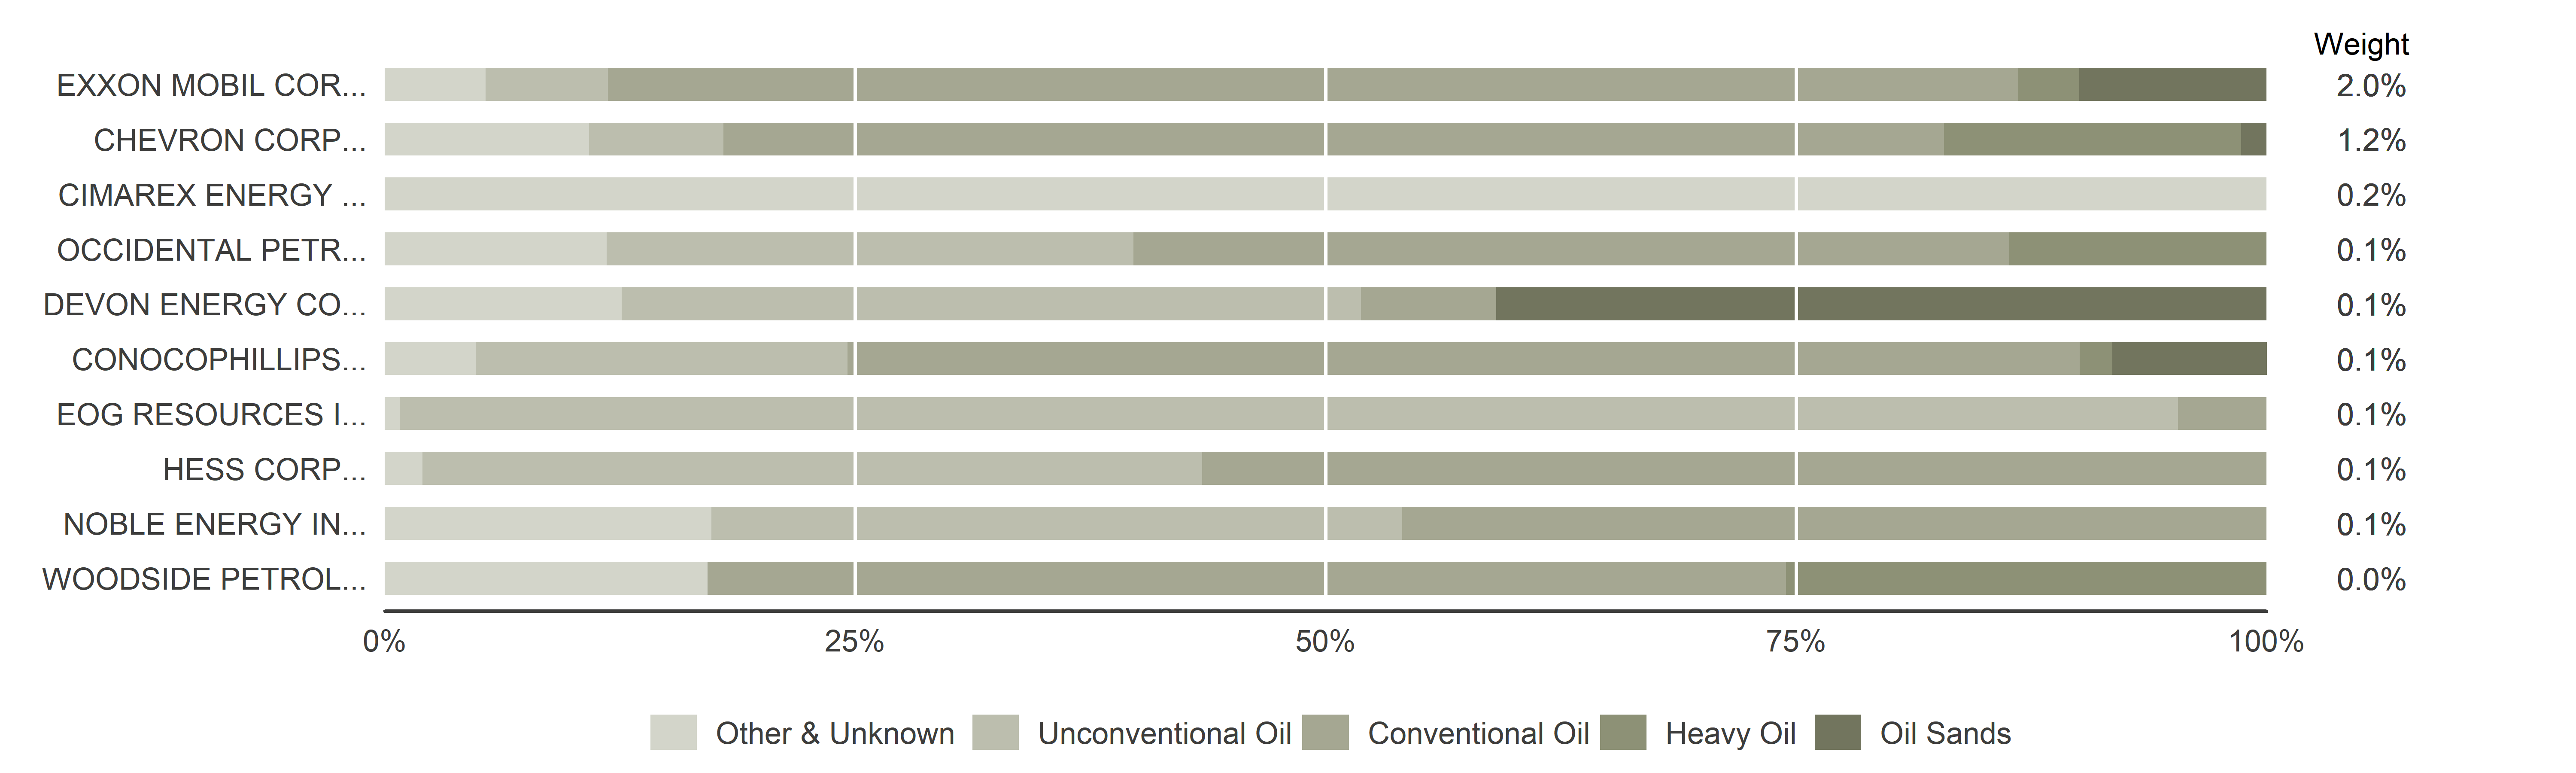
\includegraphics[trim = {0 0cm 0 0},width=1\linewidth]{CAFigures/Fig39}
	\end{center}
	
	
	\PageFooterFifth
	\newpage
	%FossilFuelSector_ALLE
	
	\section*{} % CONTRIBUTIONS OF SECURITIES TO THE RESULTS   %PowerSector_ALLS
	\HeaderDouble{CONTRIBUTIONS OF SECURITIES TO THE RESULTS}{POWER}
	
	\begin{multicols}{2}
		\textbf{The figures below show the currently planned fuel mix in 2023 for the largest holdings (by market value) of utilities in the fixed income and equity portfolios.} 
		
		
		The results are shown compared to the portfolio's currently planned fuel mix, the portfolio's target fuel mix under a 2° scenario, and the market's currently planned fuel mix (all as of 2023). The weight is the size of the total investment in each company as a percent of the total value of the fixed income portfolio. 
		
	\end{multicols}
	
	%PowerSector_CBS
	\textbf{Technology breakdown of power companies within the fixed income portfolio}
	\vspace{-.5cm}
	
	\begin{center}
		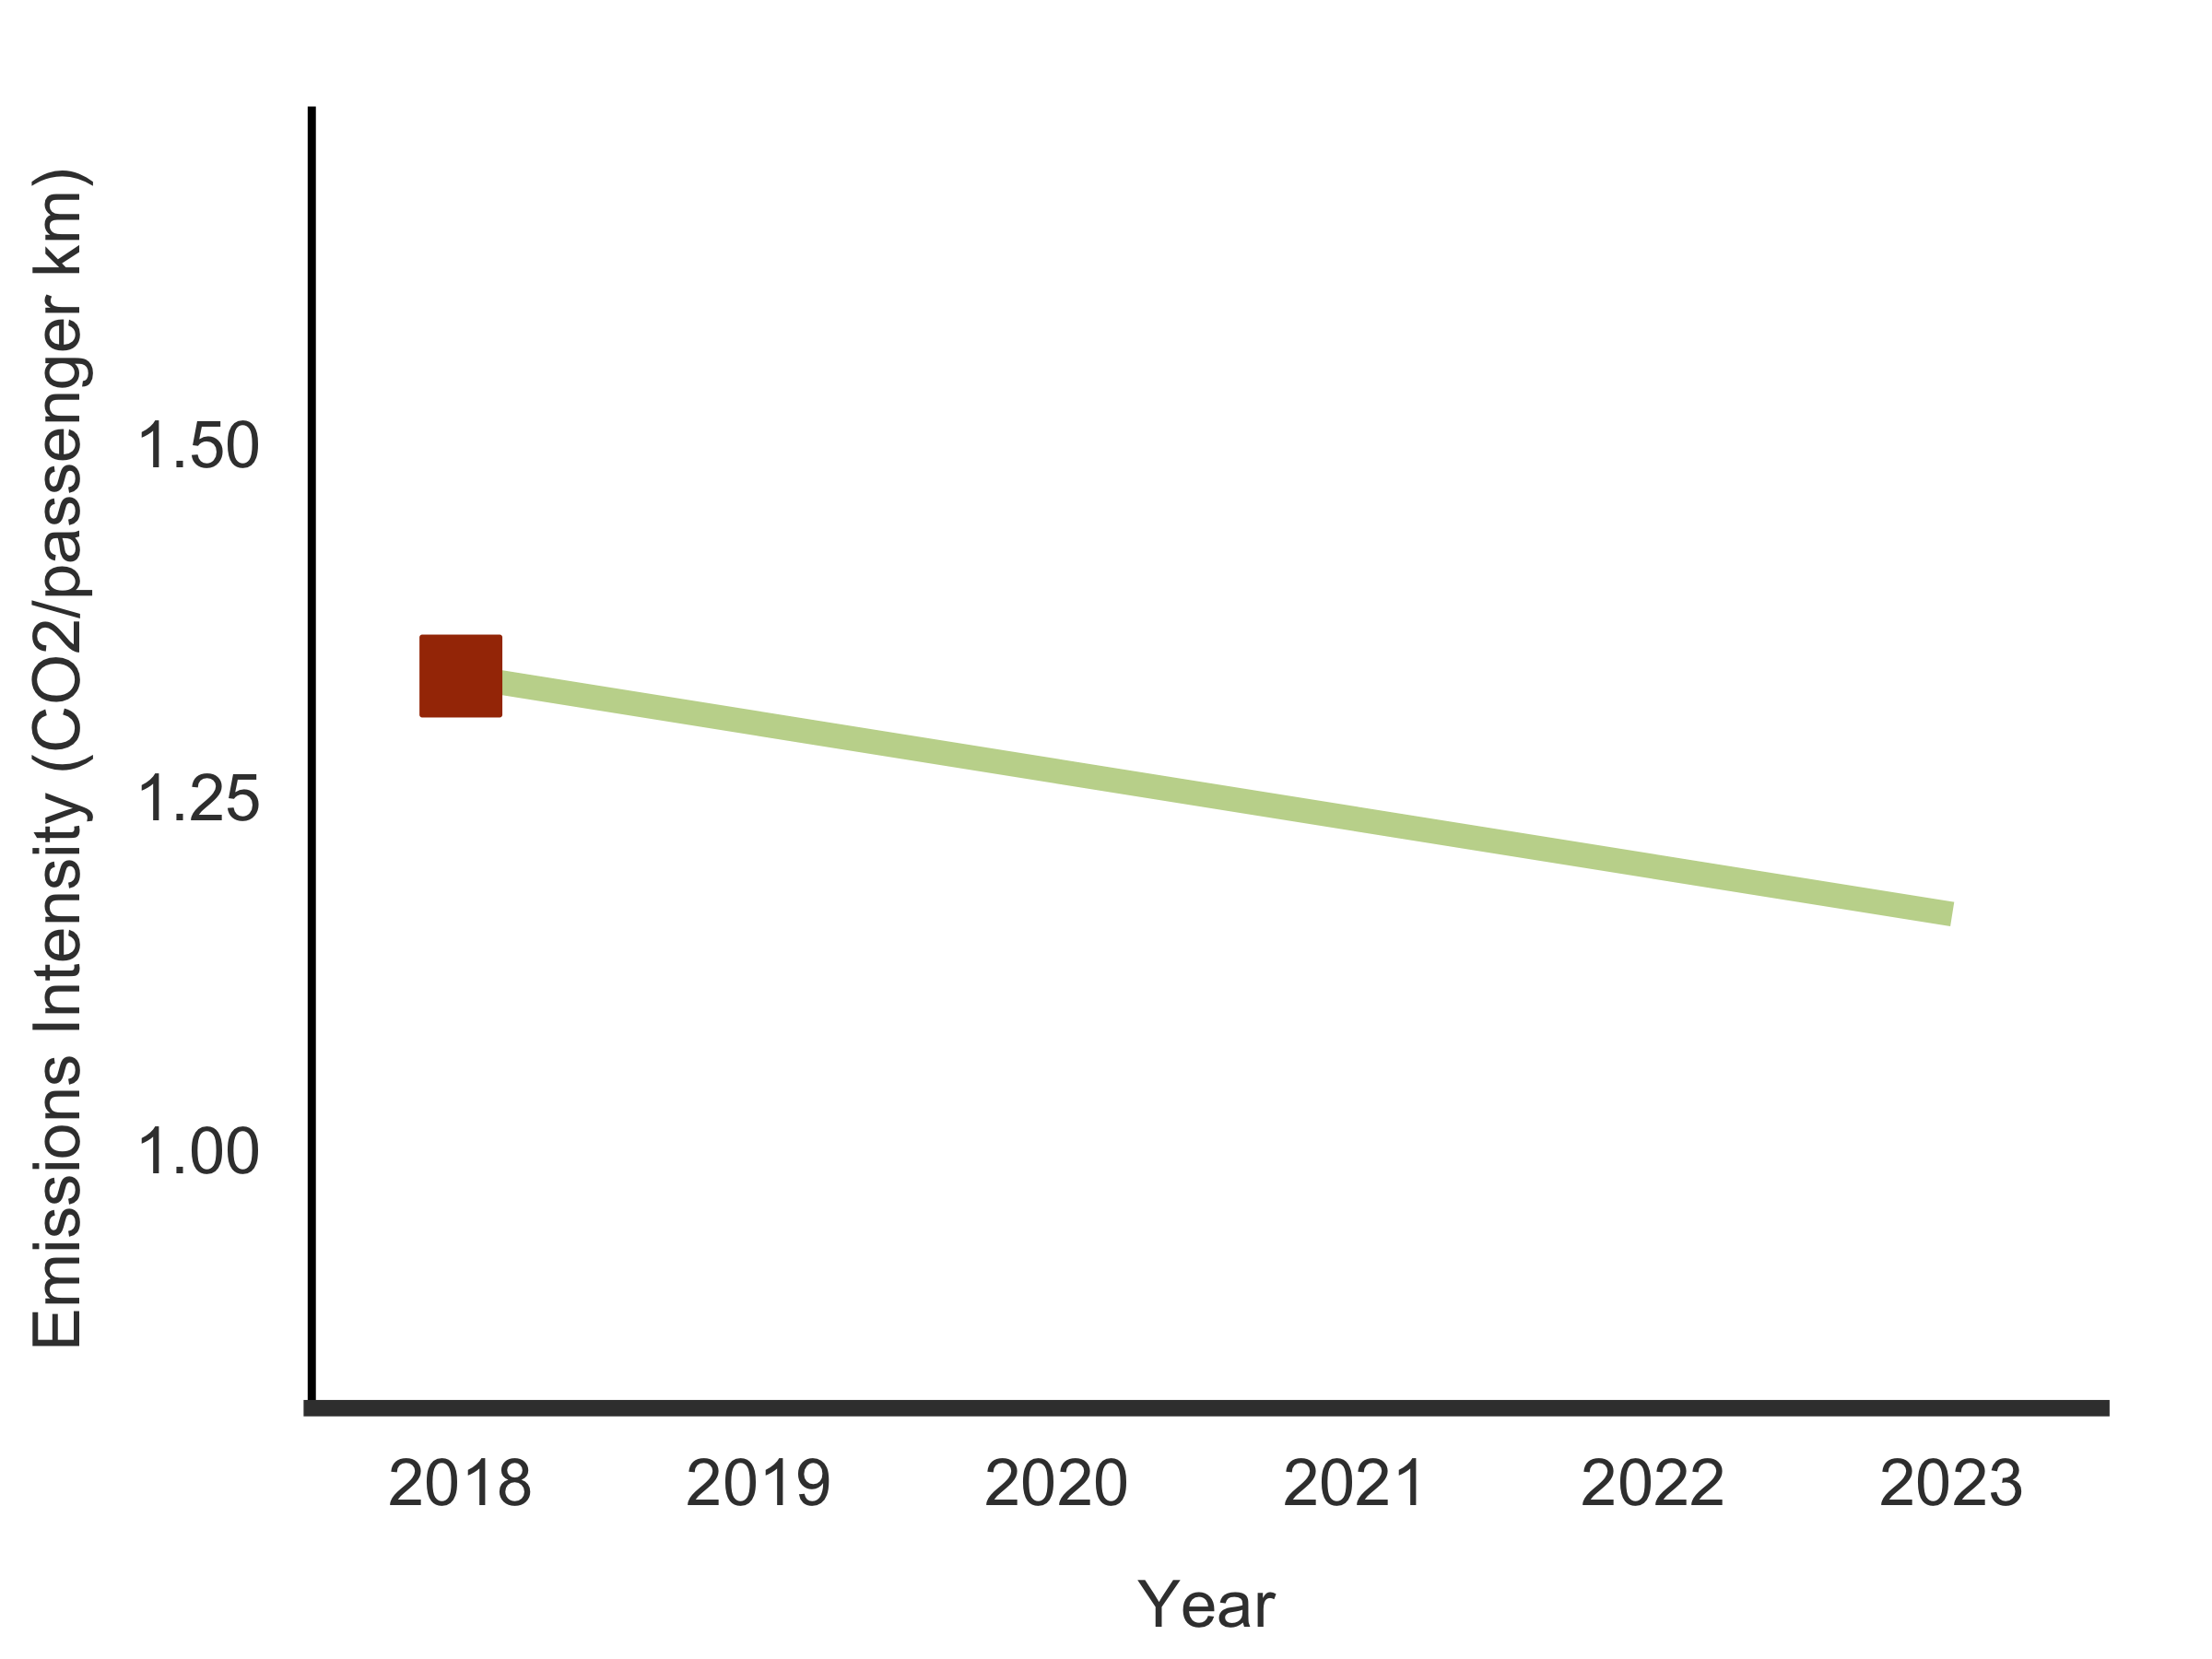
\includegraphics[trim = {0 0cm 0 0},width=1\linewidth]{CAFigures/Fig32}
	\end{center}
	%PowerSector_CBE
	%PowerSector_EQS
	\textbf{Technology breakdown of power companies within the equity portfolio}
	\vspace{-.5cm}
	
	\begin{center}
		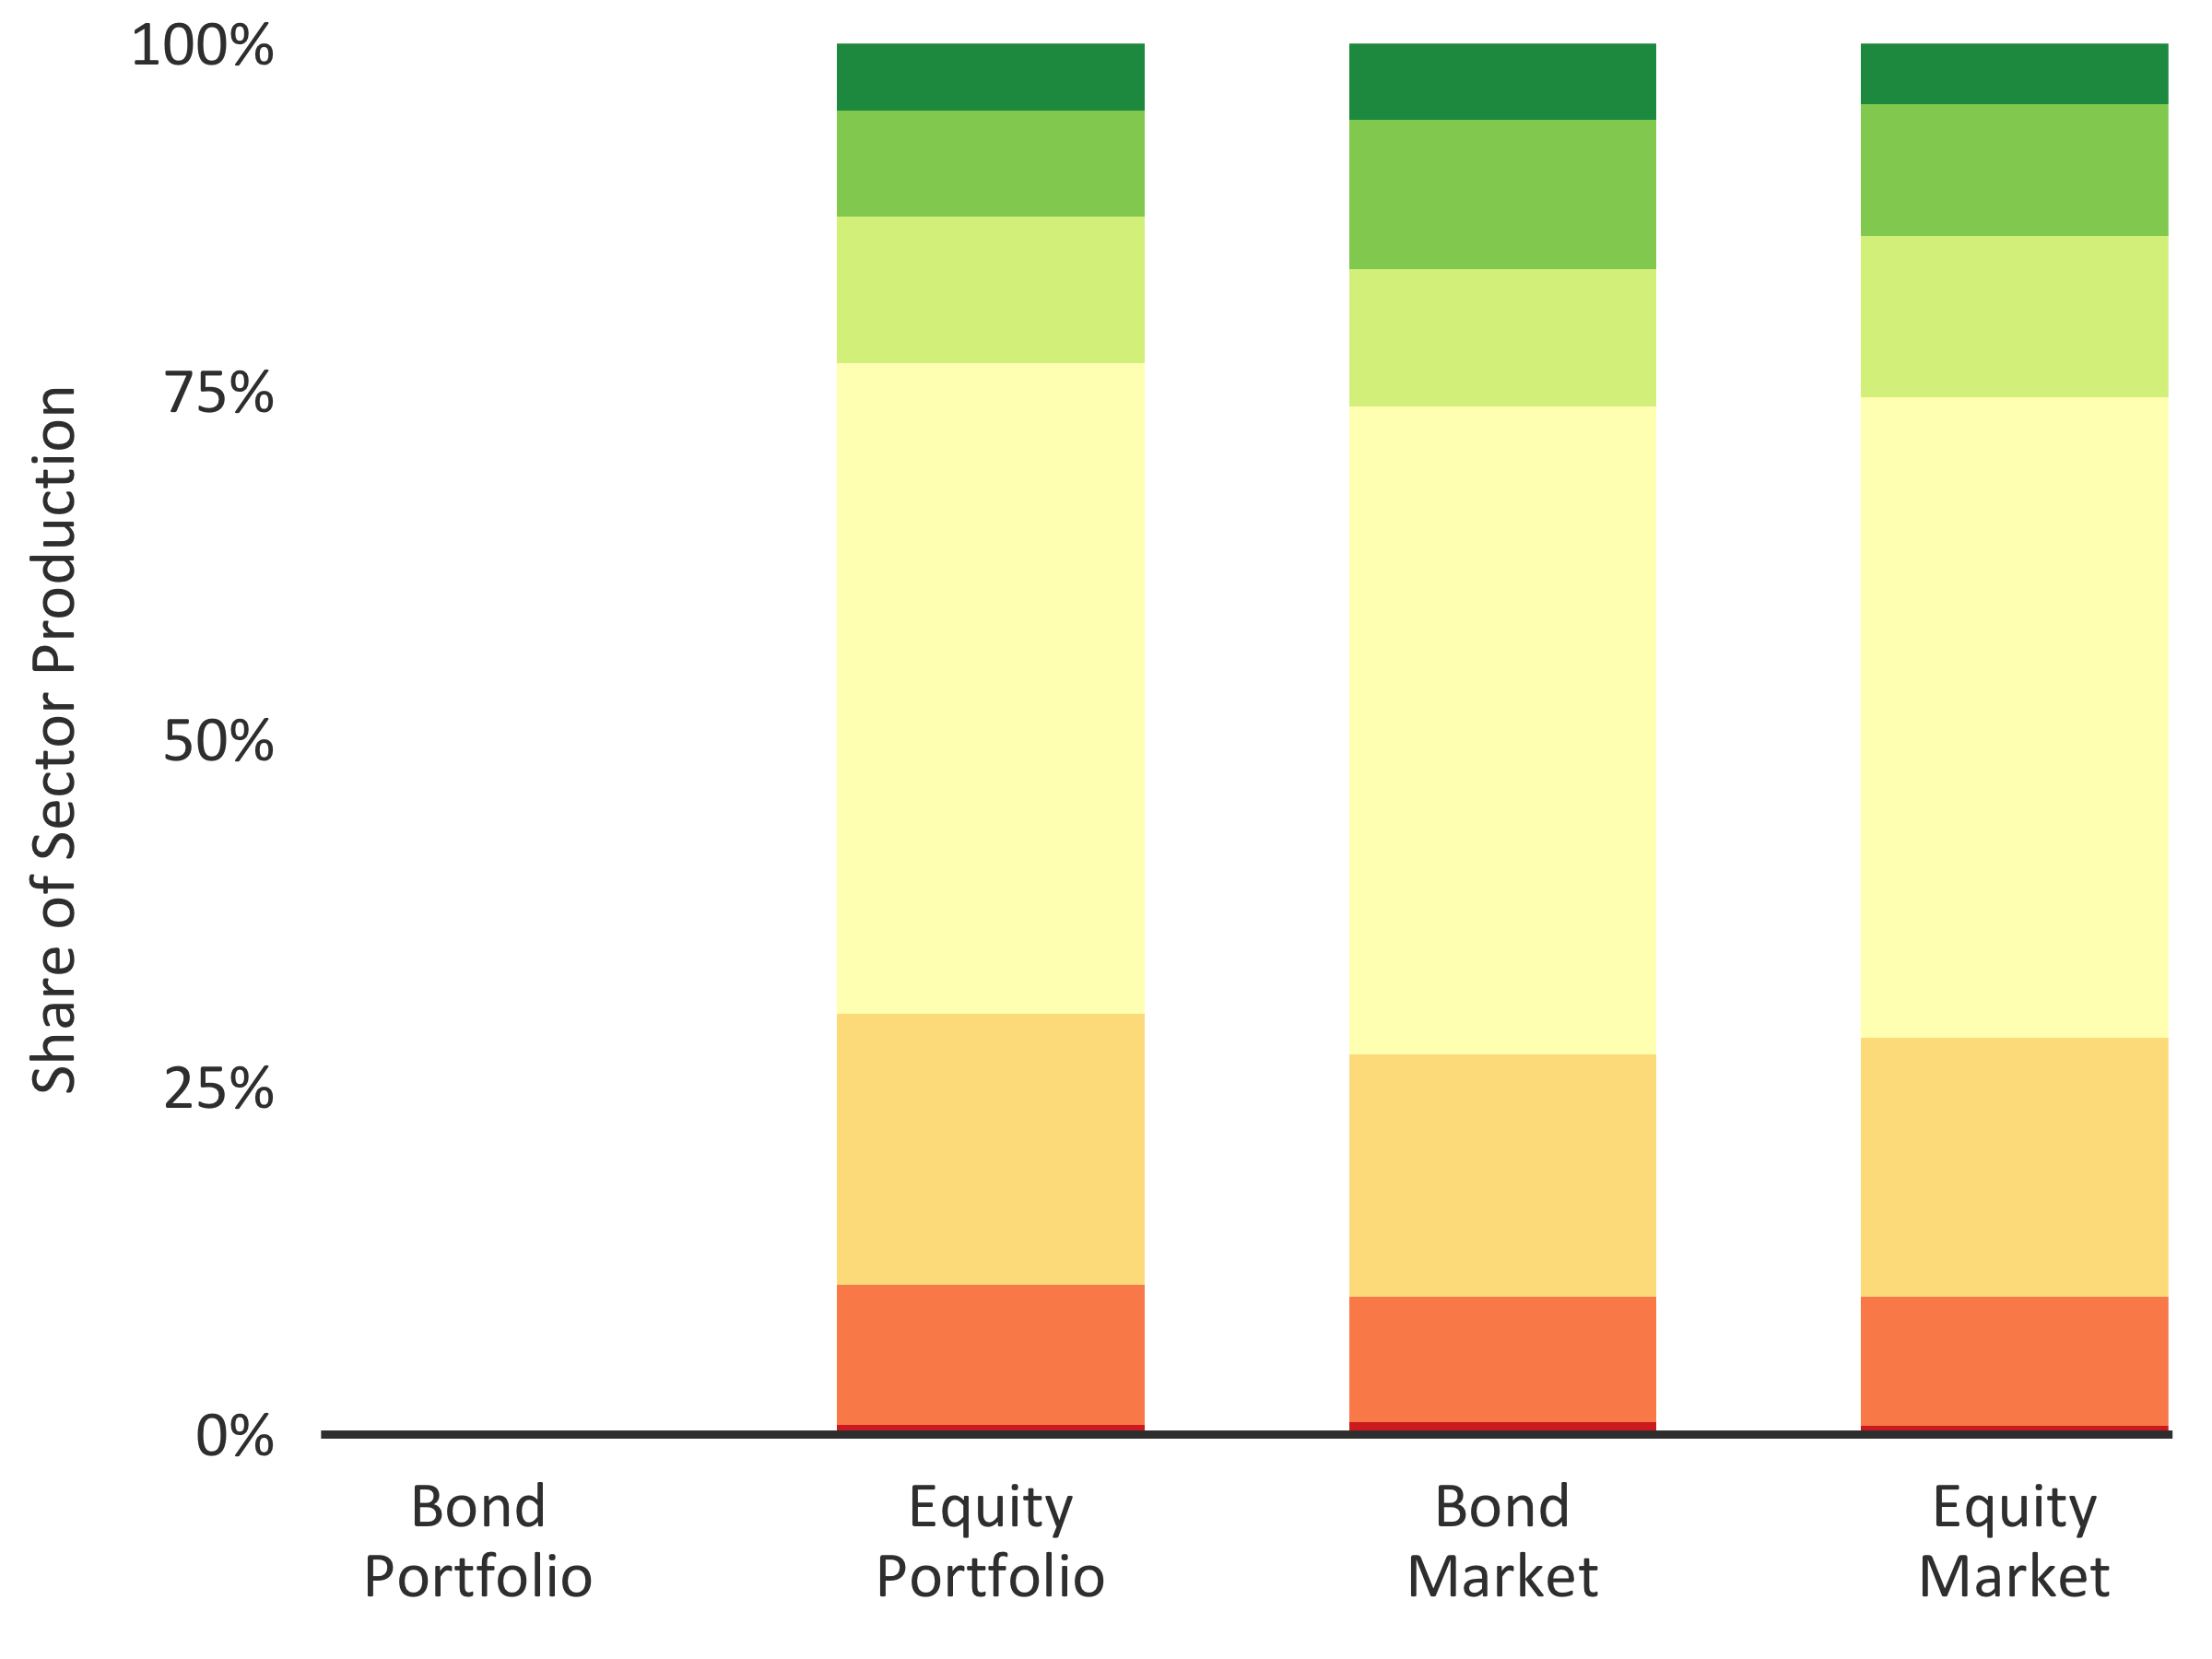
\includegraphics[trim = {0 0cm 0 0},width=1\linewidth]{CAFigures/Fig33}
	\end{center}		
	%PowerSector_EQE
	
	\PageFooterSixth
	\newpage
	%PowerSector_ALLE
	
	\section*{} % CONTRIBUTIONS OF SECURITIES TO THE RESULTS   %AutoSector_ALLS
	\HeaderDouble{CONTRIBUTIONS OF SECURITIES TO THE RESULTS}{AUTOMOTIVE}
	
	\begin{multicols}{2}
		\textbf{The figures below show the currently planned production mix of engine technologies in 2023 for the largest holdings (by market value) of automobile manufacturers in the fixed income and equity portfolios.} 
		
		
		The results are shown compared to the portfolio's currently planned production mix, the portfolio's target production mix under a 2° scenario, and the market's currently planned production mix. The weight is the size of the total investment in each company as a percent of the total value of the equity portfolio.
		
	\end{multicols}
	
	%AutoSector_CBS
	\textbf{Technology breakdown of automotive companies within the fixed income portfolio}
	\vspace{-.5cm}
	
	\begin{center}
		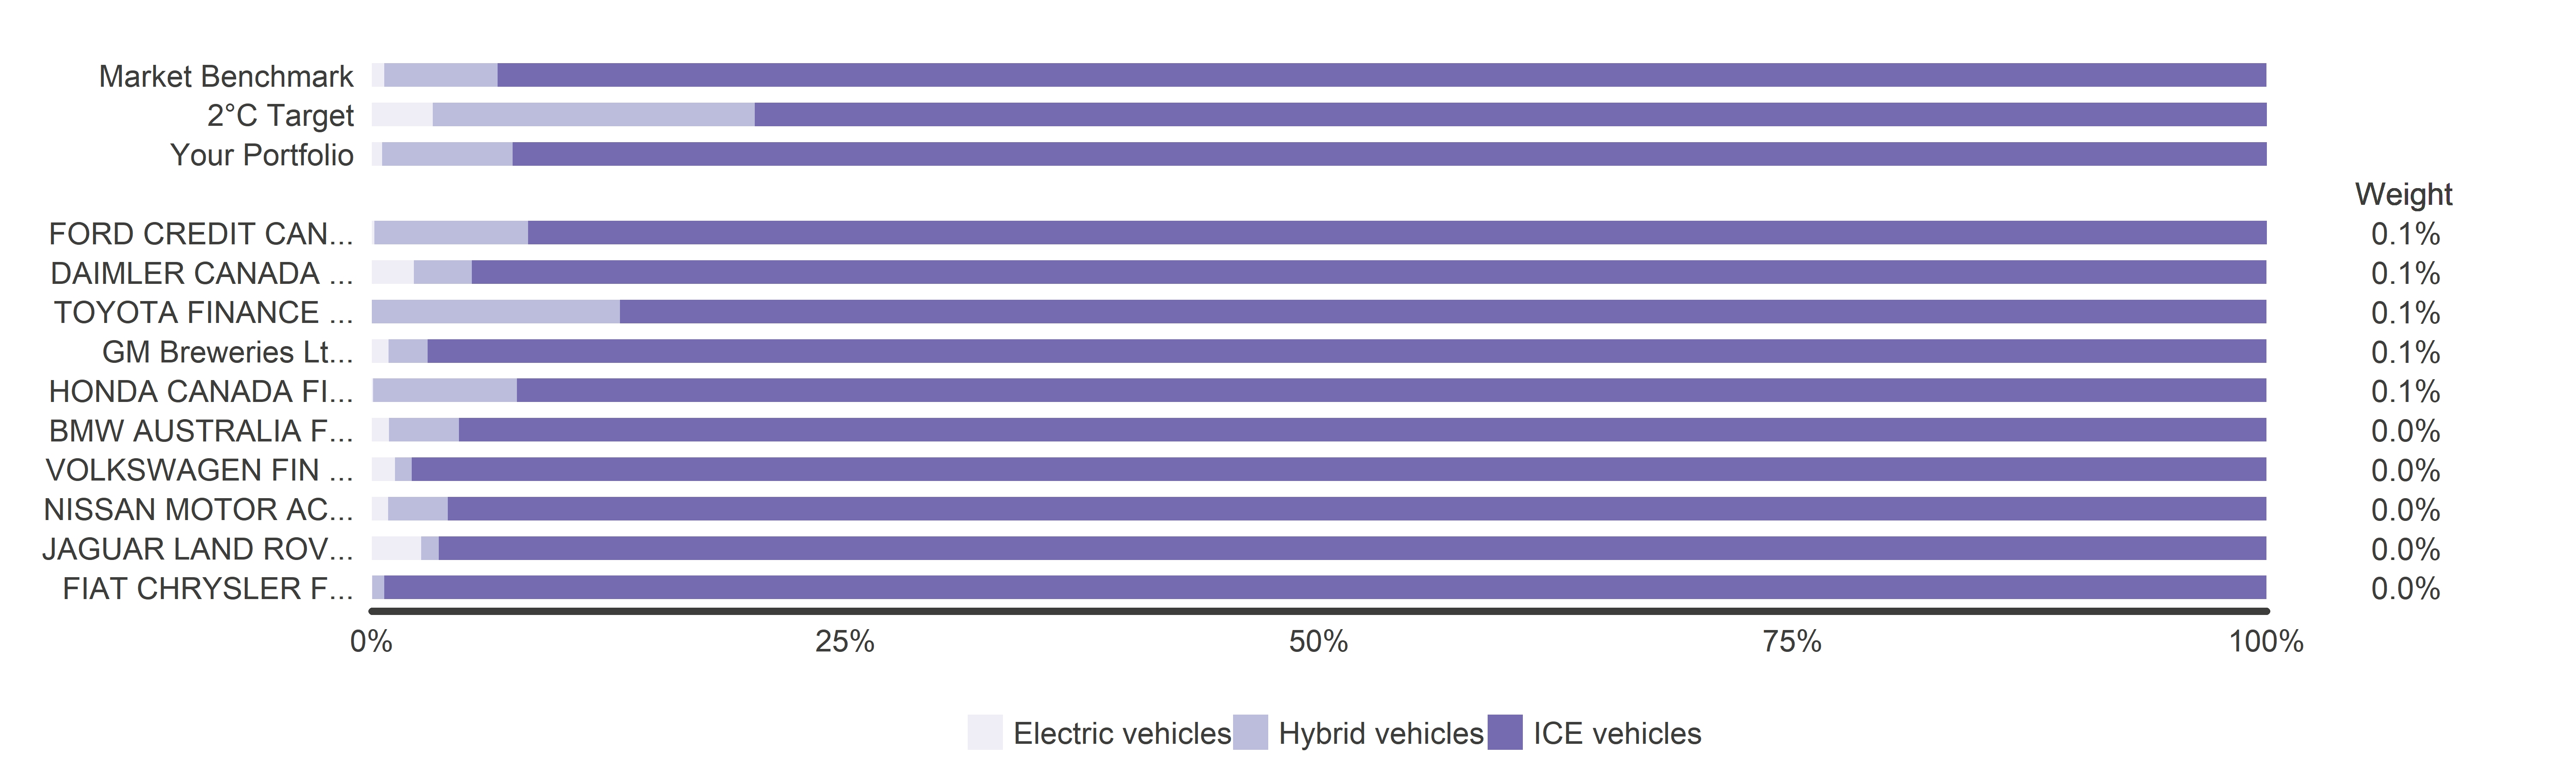
\includegraphics[trim = {0 0cm 0 0},width=1\linewidth]{CAFigures/Fig34}
	\end{center}
	%AutoSector_CBE
	
	%AutoSector_EQS
	\textbf{Technology breakdown of automotive companies within the equity portfolio}
	\vspace{-.5cm}
	
	\begin{center}
		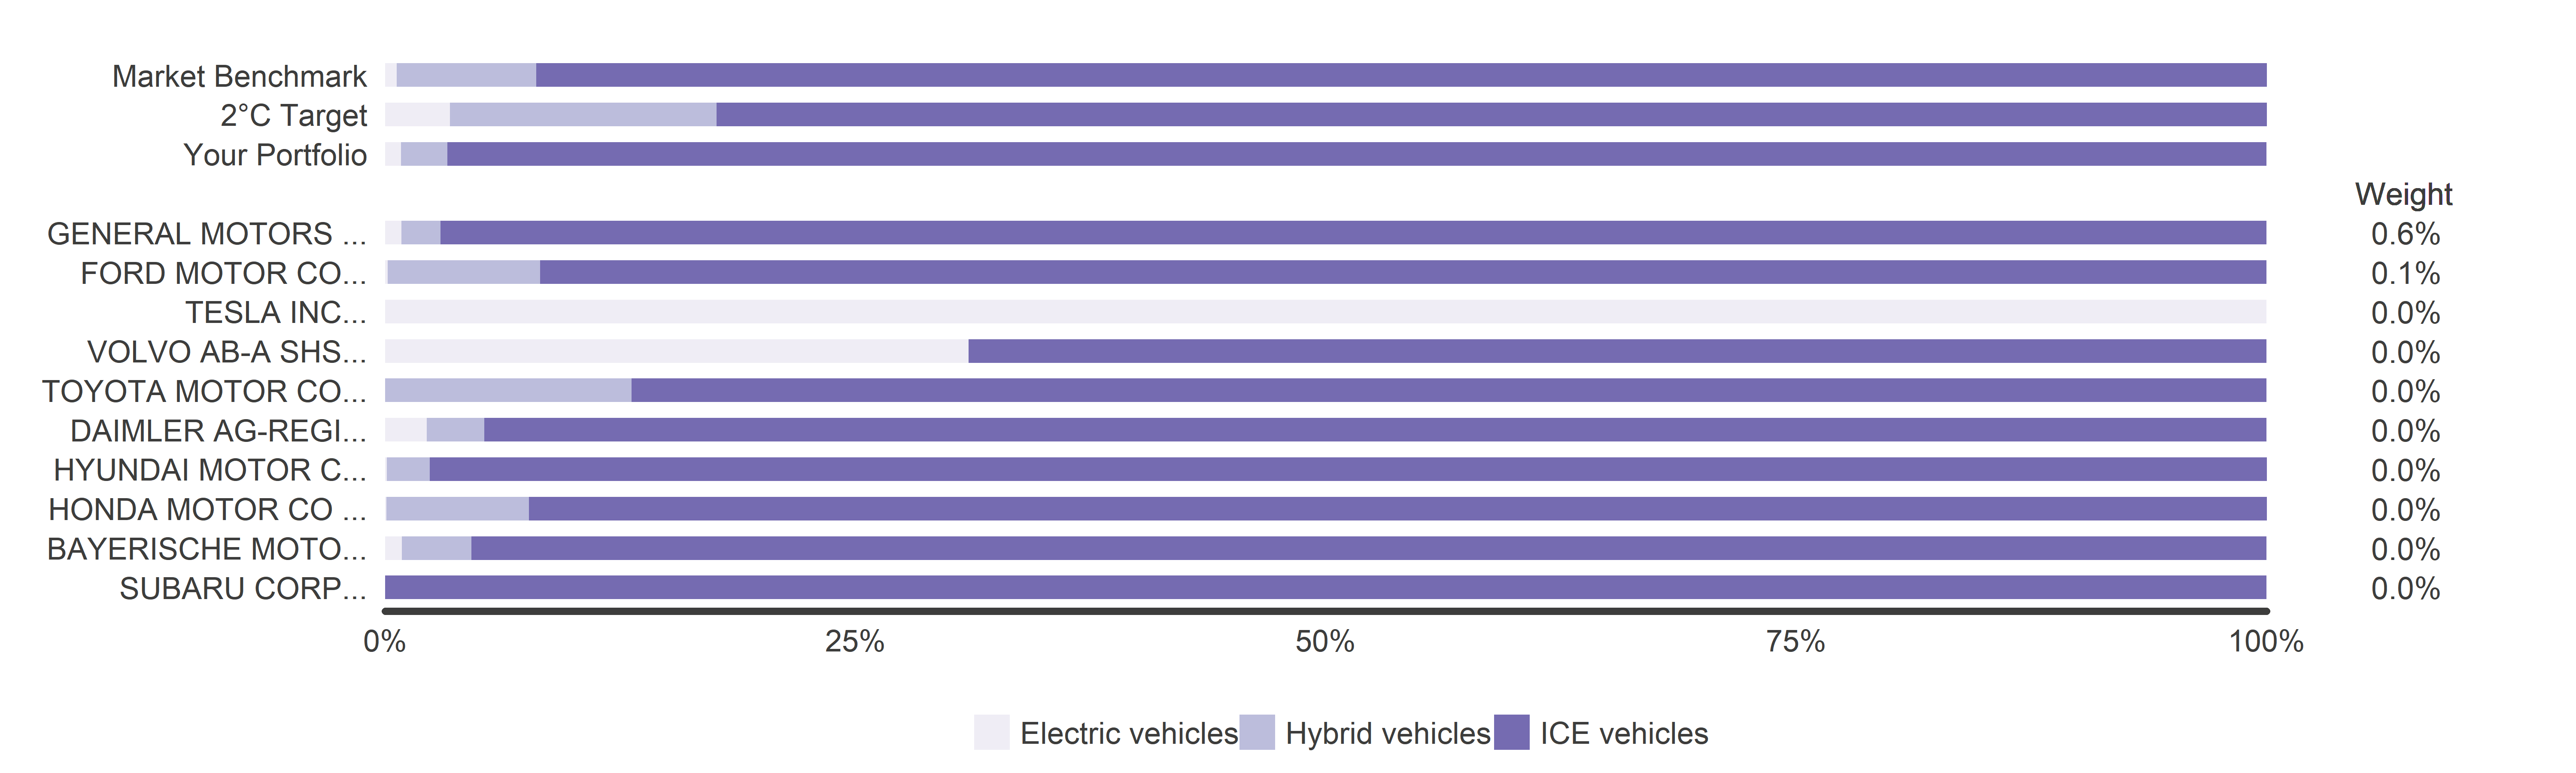
\includegraphics[trim = {0 0cm 0 0},width=1\linewidth]{CAFigures/Fig35}
	\end{center}
	%AutoSector_EQE
	
	\PageFooterSixth
	\newpage 
	%AutoSector_ALLE     CompanyChartsE
	\section*{} % 6th BACKGROUND
	\SectionHeading{SECTION 6:}{BACKGROUND TO THE MODEL}
	

	\newpage	
	\section*{} %BACKGROUND TO THE MODEL
	\HeaderSingle{BACKGROUND TO THE MODEL}
	
	\begin{multicols}{2}
		\textbf{The objective of the assessment framework applied in this scenario analysis is to measure the alignment of financial portfolios with 2°C decarbonisation pathways. The model consists of 3 key elements that are detailed in the following pages.}
		
		
		\begin{itemize}
			
			\item {Scenarios, notably 2°C scenarios, that form the basis of the analysis and define the benchmark against which portfolio trends are compared. While in theory a range of scenarios can be applied within the model, in the interest of simplification this analysis relies on the scenarios of the International Energy Agency. These provide targets for each technology at a regional level. }
			
			\item{Financial portfolios and associated financial data to allow for the portfolio assessment. Within this report, the analysis is limited to fixed income and equity portfolios. Funds within the portfolios have been identified and the underlying financial data extracted from Morningstar and included as part of the portfolio. }
			
			\item{Physical / industry `asset level data' (current and forward looking) is mapped to companies, parents, and securities. This 	allows the link between financial portfolios and industry and production data (oil and gas production, automotive production, power capacity) to be established. Consequently, this allows a comparison to the 2°C scenarios and a corresponding evaluation of the alignment of the portfolio. }
			
		\end{itemize}
	\end{multicols}
	
	
	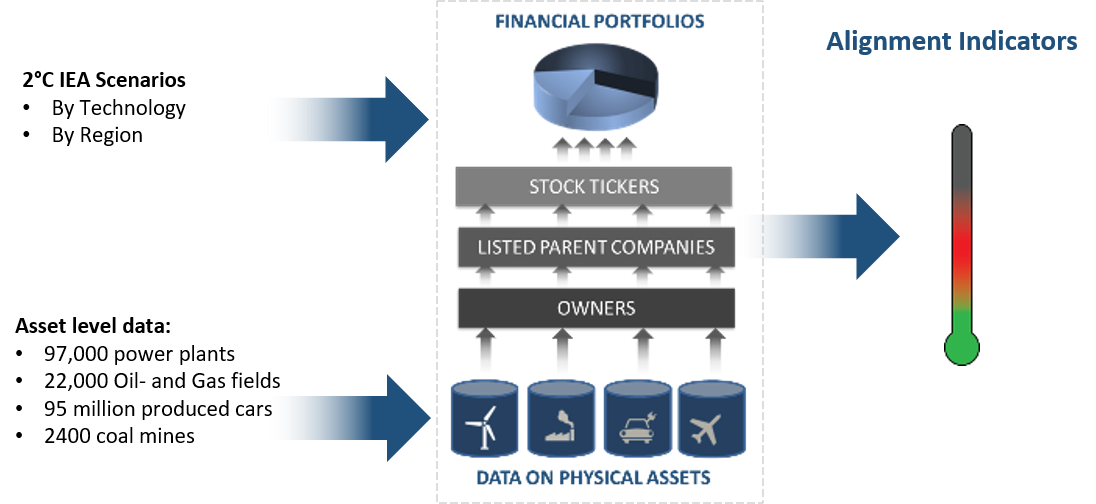
\includegraphics[trim = {0 0cm 0 0},width=1\linewidth]{ReportGraphics/SummaryChart}
	
	\begin{multicols}{2}
		\textbf{Allocation Rules.}
		Based on the financial data, the asset level data is allocated to the portfolio to quantify a representative value of what the portfolio physically owns. The assets are allocated to the portfolio based on the weight of the securities in the portfolio. 
		
		\textbf{Benchmarking.}
		Using the allocated production or capacity of technologies within the portfolio in as a starting point, an allowance based on the regional scenarios is calculated. This is extrapolated over the next 5 years to create the trajectory and this is compared to the current and future ownership. The variation of the ownership from this benchmark is used as the alignment indicator in the preceding results. 
	\end{multicols}
	
	
	
	\newpage	
	\section*{} %BACKGROUND TO THE MODEL
	\HeaderSingle{BACKGROUND TO THE MODEL}
	
	\begin{multicols}{2}
		
		
		\textbf{Assessing Alignment with a 2°C Transition Pathway. }This analysis assesses the level of alignment with a 2°C transition pathway, using two references:
		
		\begin{itemize}
			\item{\textit{The portfolio's `own' 2°C target.} This is the portfolio's target production profile `under the 2° scenario': the changes required in the production profile of the companies held in the portfolio, in order to meet the target, based on the above-described methodology. While the 2°C scenario is the focus of this analysis, the target profiles for a 4°C and a 6°C scenario are also calculated to provide further context. Since the securities held and their weight in the portfolio are identical for the portfolio and its alternative versions, comparing them shows how aligned or misaligned the current production profiles of companies held in the portfolio are with each scenario.}
			
			\item{\textit{The 2°C benchmark. }This is the target production profile of a `market benchmark' under the 2° scenario. The same principle as described above is applied to a `benchmark portfolio': the listed equity market as a whole, or the corporate fixed income market as a whole. Since the securities and their weight in the market portfolio differ from those in the portfolio, this comparison highlights `idiosyncratic' alignment or misalignment. In other words, it shows how the current composition of the portfolio affects the alignment with the different scenarios, when the first reference only stresses the changes requested from the companies.}
		\end{itemize}
		
		
		The alignment or misalignment of a portfolio's production and exposure to each technology relative to a scenario is one way to better understand an insurer's exposure to energy transition risk. If policy, technology, market, or regulatory changes occur to bring the global real economy in line with the 2°C scenario, misalignment in a given technology would likely change the financial returns associated with those underlying physical assets. However, this analysis only assesses one dimension of energy transition risks: the assets at risk in the real economy. It does not take into account the financial resilience of the company to those changes and its capacity to adapt, which would require further financial analysis.
		
		\textbf{Scenarios.} The IEA's 450 Scenario (450S) is the most well know climate scenario globally. It defines how climate-relevant technologies - 	essentially energy technologies - must be deployed by 2050 to reach a 50\% probability of limiting warming to 2°C or 3.6°F. In addition to the 450S, the IEA also defines the New Policies Scenario (NPS) and Current Policies Scenario (CPS): other technology roadmaps that correspond to a 50\% probability of maximum 4°C and 6°C warming, respectively. The 450S (also referred as the `2° scenario'), NPS (`4° scenario'), and CPS (`6° scenario') all provide forward-looking projections with enough regional detail to perform scenario analysis for 11 technologies in 3 sectors. The analysis is based on the IEA scenarios for the California Department of Insurance and covers fossil fuel extraction (oil, gas, and coal mining); production of electricity (from coal, gas, petrol, hydro, nuclear, and renewables); and, the production of cars (internal combustion engines - gasoline and diesel, hybrid, and electric).
		
		The IEA historically has assumed significant amounts of nuclear power and carbon capture and storage in their scenarios. While the IEA has updated the names and models in 2017, given that this report uses 2016 portfolio data, 2016 scenarios were applied for this analysis. In addition, the international community has accelerated their global target from the 2°C goal to `well below 2°C' with a target of 1.5°C. It is important to highlight that each investor can and may want to take an individual view on the likely decarbonization scenario that may or may not relate to the scenarios modelled by the International Energy Agency or others.
		
		The model uses the following indicators from the International Energy Agency scenario against which the portfolio is compared:
		\begin{itemize}
			\item{Electric capacity by fuel expressed in MW (e.g. renewables, coal, gas, oil, hydropower, nuclear);}
			\item{Oil production expressed in gigajoules of oil produced / year;}
			\item{Gas production expressed in gigajoules/ year;}
			\item{Coal produced expressed in mtoe / year;}
			\item{GHG emissions pathways in a sample of additional sectors (e.g. aviation, shipping, cement, steel).}
		\end{itemize}
		
		
		\textbf{Asset Level Data.} The Asset Level data is sourced from the following data providers: 
		\begin{itemize}
			\item{GlobalData (Power plant data, including plants classified as active, announced, financed, partially active, permitting, temporarily shutdown, under construction, under rehabilitation and modernization, and Oil and Gas production data and forecasts until 2018-2023, as well as coal mining data); }
			\item{WardsAuto (light passenger duty vehicles, including BAU production forecasts 2018-2023); }
			\item{Bloomberg (financial data);}
			\item{S\&P Cross-Reference Services (database matching securities to parents);}
			\item{Morningstar (database on funds). }
			
		\end{itemize}
		
		
		
		
	\end{multicols}
	
	
	
	\newpage
	\section*{} %BACKGROUND TO THE MODEL
	\HeaderDouble{IMPORTANT CONSIDERATIONS AND LIMITATIONS}{WHEN INTERPRETING THESE RESULTS }
	
	\begin{multicols}{2}
		\begin{itemize}
			\item{\textit{Stringency of scenarios.} The use of a given scenario (2°C, 4°C, and 6°C) does not constitute an assumption that this scenario is more likely to prevail than others. Similarly, the choice of IEA scenarios should not be interpreted as an endorsement of the underlying assumptions by 2Dii or the California Department of Insurance. The IEA historically has assumed significant amounts of nuclear power and carbon capture and storage in their scenarios, an assumption that is debated within the energy-climate scientific community. In addition, the international community has accelerated their global target from the 2°C goal to well below 2°C and towards 1.5°C. It is important to highlight that each insurer can and may want to take an individual view on the likely decarbonization scenario that may or may not relate to the scenarios modelled by the International Energy Agency.}
			
			\item{\textit{A snapshot rather than forecasts.} The forward-looking production data is based on current `revealed' plans from companies, and is subject to change. The estimates should thus not be interpreted as forecasts, but rather as the current plans of companies as estimated from various sources of information by industry-specific business intelligence experts - who might not know everything about the CEO's actual plans. Given the 5 year time horizon, it is likely that these plans will change in some way over time. Similarly, insurers are highly likely to alter the composition of their portfolio over time. Fixed income maturity is usually around 3-7 years. The average holding period of a stock by a fund manager is 20 months on average. However, this analysis seeks to be a point in time assessment of future exposures under current conditions.}
			
			\item{\textit{Power sector projections.} This is a measure of `locked-in' capacity, not a capacity forecast. Distinct from the production data for the fossil fuel and automotive sectors, capacity data for the power sector does not include information on planned retirements. It should therefore be interpreted as a measure of currently locked-in capacity and not as a forecast of future capacity. Retirements are not included for several reasons: First, the availability of planned retirement data is highly variable across jurisdictions and regions, to the extent that including no retirement information was deemed more representative of industry capacity than including partial data. Second, in contrast to the fossil fuel sector where oil wells, gas fields, and coal mines cease production when their resource runs out, it is possible for power plants to be announced as retired or even be retired and then resume production. Given the higher level of uncertainty around planned retirements, they are not included in the power sector projections used for this analysis, and capacity projections should thus be interpreted as the potential maximum `lock-in' from current infrastructure. For technologies projected to decline under the 2° scenario, the gap between current capacity projections and capacity consistent with the 2° scenario should be seen as an estimate of the capacity that would need to be retired to be in alignment with the 2° scenario.} 
			
			\item{\textit{Changes in plans. }The forward-looking data is based on current `revealed' plans from companies and is subject to change. The estimates should thus not be interpreted as final forecasts, but rather the current plans of companies if they don't change. Another way to interpret the results is the call for action with regard to the required change to align with the 2°C economic trend. Given the 5 year time horizon, there is a high degree of certainty that plans will still change in some way over time. Similarly, the participating financial institutions can of course alter their portfolio exposures over time. The analysis however seeks to be a point in time assessment of future exposures under current conditions.}
			\item{\textit{Ability to capture SRI strategies. }The model takes a diversified `market portfolio' as a basis, focusing on key technologies reflected in the IEA roadmaps. By extension, thematic portfolios invested in breakthrough technologies and / or SRI portfolios with a range of environmental, social, and governmental considerations may not value these elements.}
		\end{itemize}
		
		
	\end{multicols}
	\newpage		

	%	\section*{} %INTERPRETATION AND IMPLICATIONS FOR RISK
	%	\HeaderSingle{INTERPRETATION AND IMPLICATIONS FOR RISK}
	%		
	%		\begin{multicols}{2}
	%				Important in the implementation of different actions based on the 2°C scenario analysis is an understanding of the implications for risk and return of the portfolio. It is important to emphasize here that the results presented in this report are explicitly not a risk analysis. In general, the following findings can be summarized as the interaction between risk, return, and the 2°C scenario analysis. 
	%			
	%			\textbf{What is the risk of inaction?}
	%			Although the analysis focuses on alignment with the Paris Agreement in a way that contributes to the general interest, the issue can also be addressed in terms of the financial risk to the investor if the energy transition is not properly anticipated. 
	%			
	%			For investors, the main risk seems to be more pronounced if the 2°C target is not reached. Aviva and the Economist Intelligence Unit analyzed the net impairment loss for financial assets under management at approximately USD60 trillion in a 2°C scenario (Aviva 2015). The TCFD (Task Force on Climate-related Financial Disclosures) initiated by the Financial Stability Committee (FSB) calls these risks ``physical risks". If the 2°C objective is achieved, these physical risks can be reduced considerably. The cost would be limited to less than USD10 trillion if we remain below 3°C according to the same Aviva / ECIU estimates. 
	%			
	%			However, investment portfolios can then be exposed to what the TCFD calls ``transition risks" - the economic and financial risks associated with the transition to a low-carbon economy. These risks are likely to be particularly pronounced for the most CO\textsubscript{2}-emitting sectors, and thus their investors. Most of these sectors are covered by our analysis in the previous sections. 
	%			
	%			Although the 2°C scenario presented in this report is not directly a financial risk assessment, it can help to better understand the exposure to transition risk faced by investors. It makes it possible to understand whether the necessary transition will be gradual (when the production and investment plans are aligned with the 2°C scenario) or is likely to be abrupt (sudden correction linked to the introduction of new technologies or constraints legal proceedings leading to bankruptcies of established companies). All investment strategies are exposed to potential risks. The scenario analysis reveals how each strategy evaluated is an explicit or implicit bet on a 2°C, 4°C or 6°C scenario. Depending on the trajectory that will ultimately prevail, the portfolios will underperform or outperform. From the point of view of the optimization of the risk/return ratio in the long term, it is essential to be aware of the bet made.
	%			
	%			From a transition risk perspective, the following three questions are important:
	%			
	%			\begin{enumerate}
	%				\item{Is my portfolio over-exposed to transition risks by deviating from the 2°C benchmark?}
	%				\item{If this is the case, which securities in my portfolio are exposed to these risks?}
	%				\item{Should these risks arise, what are possible losses?}
	%			\end{enumerate}
	%			
	%			
	%			The answer to the first question is provided by the analysis presented in the previous pages. There are different approaches to quantifying exposure:
	%			
	%			\begin{itemize}
	%				\item{Based on the method presented in this report, it is possible to isolate the most misaligned sectors and securities with respect to a 2°C trajectory.}
	%				
	%				\item{The rating agency Moody's developed in 2016 a methodology to classify the different sectors of their fixed income universe according to the risk of downgrade due to environmental risk.}
	%			\end{itemize}
	%			
	%			
	%			\textbf{Asset Pricing and Risk} 
	%			A final question to be considered is: what is the potential value at risk within the climate relevant sectors if a 2° C scenario materializes? This requires additional financial analysis. In particular, assumptions must be made as to how the market has already (or not) integrated these risks into the current price of financial assets. There are several research papers on the subject, published by financial analysts, NGOs and consultants, covering equities and credit (2ii 2018). 
	%			
	%			In all this, it is important to emphasize that asset prices - based on market participants' assumptions about changes in the yield-risk profile of securities - do not necessarily reflect the economic risks faced by a company. Thus, the price of assets , and the risk that their valuation will decrease, does not automatically reflect the underlying risks to which the companies are exposed. On the other hand, it should be noted that the return potential is optimized when the allocation of capital is as efficient as possible. If the capital is not allocated efficiently, the absolute benefit is also reduced. Signals issued by the financial markets in the form of portfolio reallocation choices or via shareholder engagement can thus help optimize the allocation of capital in the real economy, and help maximize long-term returns.
	%		\end{multicols}
	%	
	%		
	%		\newpage	
	\section*{} %NOTES AND DISCLAIMER
	\HeaderSingle{NOTES AND DISCLAIMER}
	
	\begin{multicols}{2}
		
		\textbf{Published Research}
		
		The methodology behind this scenario analysis, the accounting rules applied, and further information to the scenarios and data can be found in the following published research papers. 
		
		Accounting Principles: http://www.mdpi.com/2071-1050/ 10/2/328 
		
		Scenario Work: http://et-risk.eu/toolbox/ scenarios/ 
		
		Asset Level Data Analysis: http://2degrees-investing.org/ IMG/pdf/assetdata\_v0.pdf
		
		\textbf{Sources for the data and scenario analysis}
		
		Automobile data are from July 2017 and is provided by WardsAuto / AutoForecastSolutions. Power data is from July 2017 and is provided by GlobalData. Oil, gas and coal production data is from July 2017 and is provided by GlobalData. When linking asset data with companies, the data is used by the data providers mentioned above and, where possible, enriched with company data from Bloomberg. All financial data, as well as identification numbers for linking company data with financial instruments, come from Bloomberg. 
		
		
		\textbf{Sources}
		
		IPCC (2018) https://www.ipcc.ch/report/ar5/
		
		FSB (2018) https://www.fsb-tcfd.org/publications/final-recommendations-report/
		
		Aviva / ECIU (2015) https://www.aviva.com/media/thought-leadership/climate-change-value-risk-investment-and-avivas-strategicresponse/
		
		FSB (2018) https://www.fsb-tcfd.org/publications/final-recommendations-report/
		
		WoodMackenzie (2018) https://www.woodmac.com/news/ editorial/carbon-intensity-not-all-assets-are-created-equal/ 
		
		
		\textbf{Disclaimer}
		
		The 2° Investing Initiative's research is provided free of charge and 2Dii does not seek any direct or indirect financial compensation for its research. 2Dii is not an investment adviser and makes no representation regarding the advisability of investing in any particular company or investment fund or other vehicle. A decision to invest in any such investment fund or other entity should not be made in reliance on any of the statements set forth on this website and the analysis results. The information and analysis contained in this research report does not constitute an offer to sell securities or the solicitation of an offer to buy, or recommendation for investment, in any securities within the United States or any other jurisdiction. The information is not intended as financial advice. The research report and website results provide general information only. The information and opinions constitute a judgment as at the date indicated and are subject to change without notice. No representation or warranty, express or implied, is made by 2Dii as to their accuracy, completeness or correctness. 2Dii does not warrant that the information is up to date, nor does it take liability for errors in third-party sourced data.
	\end{multicols}
	
	\newpage
	
	
\end{document} 

